\documentclass[preprint,3p,12pt]{elsarticle}
%\documentclass[final,3p,times]{elsarticle}
\usepackage{amsmath}
\usepackage{amssymb}
\usepackage{bm}
\usepackage{color}
\usepackage{graphicx}
\usepackage{hyperref}
\usepackage[all]{hypcap}
\usepackage[utf8x]{inputenc}
%%switch on for linenumbers%% \usepackage{lineno}
\usepackage{listings}
\usepackage{lmodern}
\usepackage{lscape}
\usepackage{xspace}

\hypersetup{
    bookmarks=true,         % show bookmarks bar?
    unicode=false,          % non-Latin characters in Acrobat�s bookmarks
    pdftoolbar=true,        % show Acrobat�s toolbar?
    pdfmenubar=true,        % show Acrobat�s menu?
    pdffitwindow=false,     % window fit to page when opened
    pdfstartview={FitH},    % fits the width of the page to the window
    pdftitle={HEPfit Manual},    % title
    pdfauthor={HEPfit Collaboration},     % author
    pdfsubject={hep-ph},   % subject of the document
    pdfcreator={TeXShop},   % creator of the document
    pdfproducer={MacTex, PDFLaTeX}, % producer of the document
    pdfkeywords={Flavour Physics} {Higgs Physics} {EW Physics} {Computational HEP}, % list of keywords
    pdfnewwindow=true,      % links in new window
    colorlinks=true,       % false: boxed links; true: colored links
    linktocpage=true,
    linkcolor=blue,          % color of internal links
    citecolor=red,        % color of links to bibliography
    filecolor=black,      % color of file links
    urlcolor=blue           % color of external links
}

\newcommand{\HEPfit}{\texttt{HEPfit}\xspace}
%\newcommand{\satoshisnotes}[1]{{\color{green}  #1}}
\newcommand{\satoshisnotes}[1]{{\color{blue}  #1}}

\definecolor{mygreen}{rgb}{0,0.6,0}
\definecolor{mygray}{rgb}{0.5,0.5,0.5}
\definecolor{mymauve}{rgb}{0.58,0,0.82}

\lstset{ %
  backgroundcolor=\color{white},   % choose the background color; you must add \usepackage{color} or \usepackage{xcolor}
  basicstyle=\footnotesize\ttfamily,        % the size of the fonts that are used for the code
  breakatwhitespace=false,         % sets if automatic breaks should only happen at whitespace
  breaklines=true,                 % sets automatic line breaking
  captionpos=none,                    % sets the caption-position to bottom
  commentstyle=\color{mygreen},    % comment style
  deletekeywords={...},            % if you want to delete keywords from the given language
  escapeinside={\%*}{*)},          % if you want to add LaTeX within your code
  extendedchars=true,              % lets you use non-ASCII characters; for 8-bits encodings only, does not work with UTF-8
  frame=single,	                   % adds a frame around the code
  keepspaces=true,                 % keeps spaces in text, useful for keeping indentation of code (possibly needs columns=flexible)
  keywordstyle=\color{blue},       % keyword style
  language=C++,                 % the language of the code
  otherkeywords={*,...},           % if you want to add more keywords to the set
  numbers=left,                    % where to put the line-numbers; possible values are (none, left, right)
  numbersep=5pt,                   % how far the line-numbers are from the code
  numberstyle=\tiny\color{mygray}, % the style that is used for the line-numbers
  rulecolor=\color{black},         % if not set, the frame-color may be changed on line-breaks within not-black text (e.g. comments (green here))
  showspaces=false,                % show spaces everywhere adding particular underscores; it overrides 'showstringspaces'
  showstringspaces=false,          % underline spaces within strings only
  showtabs=false,                  % show tabs within strings adding particular underscores
  stepnumber=1,                    % the step between two line-numbers. If it's 1, each line will be numbered
  stringstyle=\color{mymauve},     % string literal style
  tabsize=2,	                   % sets default tabsize to 2 spaces
  title=\lstname                   % show the filename of files included with \lstinputlisting; also try caption instead of title
}

\newcounter{bla}
\newenvironment{refnummer}{%
\list{[\arabic{bla}]}%
{\usecounter{bla}%
 \setlength{\itemindent}{0pt}%
 \setlength{\topsep}{0pt}%
 \setlength{\itemsep}{0pt}%
 \setlength{\labelsep}{2pt}%
 \setlength{\listparindent}{0pt}%
 \settowidth{\labelwidth}{[9]}%
 \setlength{\leftmargin}{\labelwidth}%
 \addtolength{\leftmargin}{\labelsep}%
 \setlength{\rightmargin}{0pt}}}
 {\endlist}

\journal{Computer Physics Communications}

\begin{document}

\begin{frontmatter}

%% Title, authors and addresses

%% use the tnoteref command within \title for footnotes;
%% use the tnotetext command for the associated footnote;
%% use the fnref command within \author or \address for footnotes;
%% use the fntext command for the associated footnote;
%% use the corref command within \author for corresponding author footnotes;
%% use the cortext command for the associated footnote;
%% use the ead command for the email address,
%% and the form \ead[url] for the home page:
%%
%% \title{Title\tnoteref{label1}}
%% \tnotetext[label1]{}
%% \author{Name\corref{cor1}\fnref{label2}}
%% \ead{email address}
%% \ead[url]{home page}
%% \fntext[label2]{}
%% \cortext[cor1]{}
%% \address{Address\fnref{label3}}
%% \fntext[label3]{}

\title{\HEPfit: a Code for the Combination of Indirect and Direct
  Constraints\\ on High Energy Physics Models. \\
  v1.0: Precision Electroweak Observables, Higgs Signal Strengths,\\ and Flavour Violation in the
  Standard Model and Beyond}

%\ead[url]{http://hepfit.roma1.infn.it}
\author[]{\HEPfit Collaboration \corref{hf}}
\cortext[hf]{http://hepfit.roma1.infn.it}
\ead{hepfit-support@roma1.infn.it}
\author[a]{\hspace*{-8pt}\colorbox{white}{}\hspace*{-4pt}: J.~de Blas}
\author[a]{D.~Chowdhury}
\author[b]{M.~Ciuchini}
\author[a]{O.~Eberhardt}
\author[a]{M.~Fedele}
\author[a]{E.~Franco}
\author[c]{S.~Mishima}
\author[a]{A.~Paul}
\author[d]{M.~Pierini}
\author[e]{L.~Reina}
\author[a]{L.~Silvestrini}
\author[f]{M.~Valli}
\author[g]{N.~Yokozaki}

\address[a]{INFN, Sezione di Roma, Piazzale A. Moro 2, I-00185 Roma, Italy}
\address[b]{INFN,  Sezione di Roma Tre, Via della Vasca Navale 84, I-00146 Roma, Italy}
\address[c]{Institute of Particle and Nuclear Studies, KEK, Tsukuba 305-0801, Japan}
\address[d]{CERN}
\address[e]{Physics Department, Florida State University, Tallahassee, FL 32306-4350, USA}
\address[f]{SISSA, via Bonomea 265, I-34136 Trieste, Italy and INFN, Sezione di Trieste, via Valerio 2, I-34127 Trieste, Italy}
\address[g]{Department of Physics, Tohoku University, Sendai, Miyagi 980-8578, Japan}

%%\author[a]{First Author\corref{author}}
%%\cortext[author] {Corresponding author.\\\textit{E-mail address:} firstAuthor@somewhere.edu}

\begin{abstract}
\HEPfit is a flexible %open-source
tool which, given the Standard Model or any extension, allows to \textit{i)} fit the model
parameters to a given set of experimental observables;
\textit{ii)} obtain predictions for observables.
\HEPfit can be used either in Monte Carlo mode, to perform a Bayesian Markov Chain Monte Carlo
analysis of the given model, or as a library, to obtain predictions of
observables for a given point in the parameter space of the model, allowing our computational tool to be used in
any statistical framework. In the present version, Electroweak Precision Observables have been implemented
in the Standard Model and in several New Physics scenarios.
\end{abstract}

\begin{keyword}
Model fits%%keyword1; keyword2; keyword3; etc.
\end{keyword}

\end{frontmatter}

%%switch on for linenumbers%% \linenumbers

% Computer program descriptions should contain the following
% PROGRAM SUMMARY.

{\bf PROGRAM SUMMARY}

\begin{small}
\noindent
{\em Program Title: HEPfit}                                          \\
{\em Licensing provisions(delete as appropriate): CC0 1.0/CC By 4.0/MIT/Apache-2.0/BSD 3-clause/BSD 2-clause/GPLv3/CC BY NC 3.0 }                                   \\
{\em Programming language: C++}                                   \\

{\em Supplementary material:}                                 \\
  % Fill in if necessary, otherwise leave out.

{\em Nature of problem(approx. 50-250 words): The precise calculation of many high-energy physics observables, especially with the goal to use them for a global fit to a specific model, usually involves an intricate numerical set-up. Due to their complexity, most developers do not make their programs public and it is almost impossible for the rest of the community to reproduce their results.}\\
  %Describe the nature of the problem here. \\
{\em Solution method(approx. 50-250 words):}\\
  %Describe the method solution here.
{\em Additional comments including Restrictions and Unusual features (approx. 50-250 words):}\\
  %Provide any additional comments here.
   \\

%%\begin{thebibliography}{0}
%%\bibitem{1}Reference 1         % This list should only contain those items referenced in the                 
%%\bibitem{2}Reference 2         % Program Summary section.   
%%\bibitem{3}Reference 3         % Type references in text as [1], [2], etc.
%%                               % This list is different from the bibliography at the end of 
%%                               % the Long Write-Up.
%%\end{thebibliography}
\end{small}






\tableofcontents












%%%%%%%%%%%%%%%%%%%%%%%%%%%%%%%%%%%%%
\section{Introduction}
%%%%%%%%%%%%%%%%%%%%%%%%%%%%%%%%%%%%%

Searching for New Physics (NP) in the LHC era requires combining
experimental and theoretical information from many sources to optimize
the NP sensitivity. NP searches, even in the absence of a positive
signal, provide useful information which puts constraints on the
viable parameter space of any NP model. Should a NP signal emerge at
future LHC runs or elsewhere, the combination of all available
information remains a crucial step to pin down the actual NP model.
NP searches at LHC require extensive detector simulations and are
usually restricted to a subset of simplified NP models. Given the high
computational demand of direct searches, it is crucial to explore only
regions of the parameter space compatible with other constraints. In
this respect, indirect searches can be helpful and make the study of
more general models viable.

\HEPfit aims at providing a tool which allows to combine all
available information to select allowed regions in the parameter space
of any NP model. To this end, it can compute many observables with
state-of-the-art theoretical expressions in a set of models which can
be extended by the user. It also offers the possibility of sampling
the parameter space using a Markov Chain Monte Carlo implemented using
the BAT library~\cite{arXiv:0808.2552}. Alternatively, \HEPfit can be
used as a library to obtain predictions of the observables in any
implemented model. This allows to use \HEPfit in any statistical
framework.

This is the first public release with a limited set of observables and
models, which we plan to enlarge. The code is released under the GNU
General Public License, so that contributions from users are possible
and welcome. In particular, the present version provides Electro Weak
Precision Observables (EWPO) in the SM and in several parametrizations
of NP contributions. In the near future, we plan to add flavour
observables and several incarnations of the Minimal Supersymmetric
Standard Model (MSSM).

The paper is organised as follows. In Section~\ref{sec:Physics} we
summarize models and observables implemented in the present
version. In Section~\ref{sec:Code} we describe the structure of our
code. Section~\ref{sec:Usage} contains the instructions for using our
code and some examples. In Section~\ref{sec:Comparison} we compare our
numerical results with other existing public codes.

Updated information and online documentation can be found at the
\HEPfit collaboration web site~\cite{website}.



%\section{Physics Content}
%\label{sec:Physics}

%%%%%%%%%%%%%%%%%%%%%%%%%%%%%%%%%%%%%
\section{Models}
\label{sec:Models}
%%%%%%%%%%%%%%%%%%%%%%%%%%%%%%%%%%%%%

%%%%%%%%%%%%%%%%%%%%%%%%
\subsection{Standard Model}
\label{sec:SM}
%%%%%%%%%%%%%%%%%%%%%%%%
Marco Ciuchini

%%%%%%%%%%%%%%%%%%%%%%%%
\subsection{Two-Higgs-Doublet models}
\label{sec:THDM}
%%%%%%%%%%%%%%%%%%%%%%%%

One of the most straightforward extensions of the Standard Model is the Two-Higgs-Doublet model (THDM) \cite{Lee:1973iz,Gunion:2002zf,Branco:2011iw}. No fundamental theorem forbids to add a second scalar doublet to the Standard Model particle content. The THDM can offer a solution to problems like the stability of the scalar potential up to very large scales (see e.g. \cite{Chowdhury:2015yja}), electroweak baryogenesis (see e.g. \cite{Bochkarev:1990fx,Nelson:1991ab,Dorsch:2013wja}) or some conflicting flavour measurements, all of which cannot be solved in the Standard Model. Furthermore, it could emerge as an effective description of more complicated models like supersymmetric models, which necessarily contain two Higgs doublets. (The minimal supersymmetric Standard Model is presented in the next chapter.)

There are several THDM variants with different phenomenological implications. At the moment \HEPfit contains the versions which exclude flavour-changing neutral currents at tree-level as well as CP violation in the Higgs sector. In order to fulfil the first demand, an additional softly broken $Z_2$ symmetry is assumed, which can be chosen in four different ways; thus these versions are called type I, type II, type X and type Y. (The THDM of type II contains the scalar Higgs part of supersymmetric models.) The four types only differ in the Yukawa couplings of the Higgs fields; the corresponding assignments can be found in Table \ref{tab:THDMtypes}, where $Y^f_j$ denotes the coupling of one of the two Higgs doublets $\Phi_j$ (j=1,2) to the fermion field $f$.

\begin{table}[htb]
  \centering
\caption{Yukawa couplings in the four possible $Z_2$ symmetric 2HDM types.}\vspace{0.2cm}
  \begin{tabular}{|l|l|l|l|}
    \hline
      Type I & Type II & Type X (``lepton specific'') & Type Y (``flipped'') \\
    \hline
      $Y^b_{1}\equiv 0$, $Y^e_{1}\equiv 0$ & $Y^b_{2}\equiv 0$, $Y^e_{2}\equiv 0$ & $Y^b_{1}\equiv 0$, $Y^e_{2}\equiv 0$ & $Y^b_{2}\equiv 0$, $Y^e_{1}\equiv 0$ \\
      \hline
  \end{tabular}
 \label{tab:THDMtypes}
\end{table} 

By definition, $Y_1^u \equiv 0$ for all four types. In the configuration file \texttt{THDM.conf}, one has to choose the THDM type setting the flag \texttt{modelTypeflag} to \texttt{type1}, \texttt{type2}, \texttt{typeX} or \texttt{typeY}.

Hence we can write the Higgs potential for $\Phi_1$ and $\Phi_2$ as

\begin{align}
V_H^\text{\tiny{THDM}} & = m_{11}^2\Phi_1^\dagger\Phi_1^{\phantom{\dagger}}
 	+m_{22}^2\Phi_2^\dagger\Phi_2^{\phantom{\dagger}}
 	-m_{12}^2\left[ \Phi_1^\dagger\Phi_2^{\phantom{\dagger}}
 		+\Phi_2^\dagger\Phi_1^{\phantom{\dagger}}\right] 
	+\tfrac12 \lambda_1(\Phi_1^\dagger\Phi_1^{\phantom{\dagger}})^2 
	+\tfrac12 \lambda_2(\Phi_2^\dagger\Phi_2^{\phantom{\dagger}})^2 \nonumber \\
&\phantom{{}={}}
 	+\lambda_3(\Phi_1^\dagger\Phi_1^{\phantom{\dagger}})
 		(\Phi_2^\dagger\Phi_2^{\phantom{\dagger}})
 	+\lambda_4(\Phi_1^\dagger\Phi_2^{\phantom{\dagger}})
 		(\Phi_2^\dagger\Phi_1^{\phantom{\dagger}})
	+\tfrac12 \lambda_5^{} \left[ (\Phi_1^\dagger\Phi_2^{\phantom{\dagger}})^2
 		+(\Phi_2^\dagger\Phi_1^{\phantom{\dagger}})^2 \right] \label{eq:THDMVH}
\end{align}
 
and the Yukawa part of the Lagrangian as
 
\begin{align}
{\cal L}_Y^\text{\tiny{THDM}} &= -Y^u_2 \bar Q_{\textit{\tiny{L}}} \tilde\Phi_2 u_{\textit{\tiny{R}}} -\sum\limits_{j=1}^2 \left[ Y^d_j \bar Q_{\textit{\tiny{L}}} \Phi_j d_{\textit{\tiny{R}}} +Y^e_j \bar L_{\textit{\tiny{L}}} \Phi_j \ell_{\textit{\tiny{R}}}\right] + {\text{H.c.}} \nonumber ,
\end{align}
 
where one of the choices from Table \ref{tab:THDMtypes} has to be applied.

The THDM contains five physical states, two of which are neutral and even under CP transformations, one is neutral and CP-odd, and the remaining two carry the electric charge $\pm$1 and are degenerate in mass. We assume that the 125 GeV resonance measured at the LHC is the lighter CP-even Higgs $h$, while the other particles are labelled $H$, $A$ and $H^\pm$, respectively.
The eight parameters from the Higgs potential \eqref{eq:THDMVH} can be transformed into physical parameters:

\begin{itemize}
\item the vacuum expectation value $v$,
\item the lighter CP-even Higgs mass $m_h$,
\item the heavier CP-even Higgs mass $m_H$,
\item the CP-odd Higgs mass $m_A$,
\item the charged Higgs mass $m_{H^+}$,
\item the mixing angle $\alpha$,
\item the mixing angle $\beta$ and
\item the soft $Z_2$ breaking parameter $m_{12}^2$ from \eqref{eq:THDMVH}.
\end{itemize}

$G_F=1/(\sqrt{2} v^2)$ and $m_h$ are defined in the Standard Model configuration file. For practical reasons, the \HEPfit implementation uses $\beta-\alpha$ and $\log_{10}\tan\beta$ instead of $\alpha$ and $\beta$ and squared $H$, $A$ and $H^+$ masses. The THDM configuration file contains as an additional parameter the theoretical uncertainty of the observable ${\rm Br}(\bar{B}\to X_s\gamma)$.

\begin{table}[tb]
 \centering
 \caption{THDM parameters}\vspace{0.2cm}
  \begin{tabular}{|l|l|}
    \hline
      \textbf{Parameter} & \textbf{\HEPfit name} \\
    \hline
      $\log_{10}\tan\beta$ & \tt{logtb}\\
    \hline
      $\beta-\alpha$ & \tt{bma}\\
    \hline
      $m_H^2$ & \tt{mHh2}\\
    \hline
      $m_A^2$ & \tt{mA2}\\
    \hline
      $m_{H^+}^2$ & \tt{mHp2}\\
    \hline
      $m_{12}^2$ & \tt{m12\_2}\\
    \hline
      $\Delta _{\text{\tiny{theo}}}{\rm Br}(\bar{B}\to X_s\gamma)$ & \tt{bsgamma\_theoryerror}\\
    \hline
  \end{tabular}
 \label{tab:HandAsearchlimits}
\end{table} 

%%%%%%%%%%%%%%%%%%%%%%%%
\subsection{Minimal Supersymmetric Standard Model}
\label{sec:MSSM}
%%%%%%%%%%%%%%%%%%%%%%%%

The supersymmetry (SUSY) is one of the leading candidates for the physics beyond the standard model, which guarantees the absence of the quadratic divergence in the Higgs potential. The minimal SUSY extension of the SM is called the minimal supersymmetric standard model (MSSM). In the MSSM, the three gauge couplings unify around $2\cdot 10^{16}$ GeV, suggesting the existence of the grand unified theory (GUT)~\cite{Georgi:1974sy, Pati:1974yy}.
 
In the MSSM, SM fields are extended to chiral superfields, which have both scalar fields and fermion fields. The SM gauge bosons are contained in the vector superfields, which also contain fermions, gauginos. There are two Higgs superfields, which are required to write the all %?correct?
Yukawa couplings and avoid gauge anomalies. The chiral superfields having $SU(3)_C \times SU(2)_L \times U(1)_Y$ quantum numbers are summarized as 
\begin{eqnarray}
&& Q_i: ({\bf 3}, {\bf 2},1/6), \ \bar U_i: ({\bf \bar 3}, {\bf 1}, -2/3), \  \bar D_i: ({\bf \bar 3}, {\bf 1}, 1/3),  \nonumber \\ 
&& L_i: ({\bf 1}, {\bf 2}, -1/2),  \ \bar E_i:({\bf 1},{\bf 1},1), \nonumber \\
&& H_u: ({\bf 1},{\bf 2},1/2), \ H_d:({\bf 1}, {\bf 2},-1/2),
\end{eqnarray}
where $i(=1 \dots 3)$ represents a generation number.
%
The Lagrangian of the MSSM is given by\,\footnote{
We have omitted the QCD $\theta$-term as well as CP-violating terms involving dual-tensors.
}
\begin{eqnarray}
\mathcal{L} = \int d^4 \theta \, K_{\rm MSSM}  + \left[ 
\int d^2 \theta \, W_{\rm MSSM}  + \frac{1}{4} \int d^2 \theta (\mathcal{W}_{\alpha})_A (\mathcal{W}^{\alpha})_A + h.c.
\right] + \mathcal{L}_{\rm soft},
\end{eqnarray}
where $K_{\rm MSSM}$, $W_{\rm MSSM}$ and $(\mathcal{W}_{\alpha})_A$
are the K{\" a}hler potential, superpotential and gauge field-strength superfields, respectively, 
and $\mathcal{L}_{\rm soft}$ consists of soft SUSY breaking terms. 
The field-strength superfields, $(\mathcal{W}_{\alpha})_1$, $(\mathcal{W}_{\alpha}^k)_2$ $(k=1\dots 3)$ and $(\mathcal{W}_{\alpha}^I)_3$\,$(I=1\dots 8)$, consist of the vector superfields of $U(1)_Y$, $SU(2)_L$ and $SU(3)_C$, respectively. 
In the limit of $\mathcal{L}_{\rm soft}=0$, the Lagrangian is invariant under the SUSY transformation, 
and $\mathcal{L}_{\rm soft} \neq 0$ does not reintroduce quadratic divergences.
%

\vspace{10pt}
The superpotential  with the conserved $R$-parity is 
\begin{eqnarray}
W_{\rm MSSM} = \epsilon_{ab} \left[ \mu H_u^a H_d^b +  (Y_E)_{ij} H_d^a L^b_i \bar E_j
+  (Y_D)_{ij} H_d^a Q^b_i \bar D_j
+  (Y_U)_{ij} Q^a_i H_u^b \bar U_j
\right],
\end{eqnarray}
where $a,b$ are gauge indices of $SU(2)_L$, $\epsilon_{12}=-\epsilon_{21}=1$ and $\epsilon_{11}=\epsilon_{22}=0$. Here, we present only renormalizable terms. The $R$-parity is defined as
\begin{eqnarray}
R_P = (-1)^{3(B-L)+2 s},  
\end{eqnarray}
where $B$ and $L$ are baryon number and lepton number, and $s$ is the spin.
The $R$-parity guarantees the stability of the lightest SUSY particle (LSP) and prevents the proton decay.\footnote{
%
Nonrenormalizable operators, $QQQL$ and $\bar U \bar U \bar D\bar E$, which can not be prohibited by the $R$-parity induce the proton decay with an unacceptable life-time even if they are suppressed by the Planck mass~\cite{Murayama:1994tc,Harnik:2004yp}. Therefore, we need an additional mechanism or symmetry to suppress those operators further. 
%
}
Due to the $R$-parity, the lightest neutralino is often a candidate for dark matter, depending on the gravitino mass. %?put the definition of and motivation for RP before the superpotential?

%\vspace{10pt}
The soft SUSY breaking terms contain gaugino mass terms, sfermion mass terms, 
trilinear couplings and the Higgs $B$-term. 
The gaugino mass terms are given by
\begin{eqnarray}
\label{eq:Lsoft_gaugino}
-\mathcal{L}_{\rm soft} \ni  \frac{1}{2} 
\left( M_{1} \lambda_{\tilde b} \lambda_{\tilde b} +  M_{2} \lambda_{\tilde w}^k \lambda_{\tilde w}^k 
+ M_{3} \lambda_{\tilde g}^I \lambda_{\tilde g}^I + h.c. \right),
\end{eqnarray}
where $\lambda_{\tilde b}$, $\lambda_{\tilde w}^k$ and $\lambda_{\tilde g}^I$ are bino, wino and gluino, respectively, and $M_1$, $M_2$ and $M_3$ are complex parameters. Although $M_1$, $M_2$ and $M_3$ are free parameters in general,
the relation $M_1: M_2: M_3 \simeq \frac{5}{3} g_Y^2: g_2^2: g_3^2$ is hold at a given renormalization scale in a case that the gaugino masses unify at the GUT scale,\footnote{
For instance, in minimal gauge mediation and constrained MSSM (CMSSM), the gaugino masses satisfy this relation.
}
where $g_Y$, $g_2$ and $g_3$ are gauge coupling constants of $U(1)_Y$, $SU(2)_L$ and $SU(3)_C$, respectively. 


%\vspace{10pt}
The trilinear couplings and Higgs $B$-term are give by
\begin{eqnarray}
-\mathcal{L}_{\rm soft} &\ni& \epsilon_{ab} \Bigl[ B_\mu H_u^a H_d^b +  (T_E)_{ij} H_d^a L^b_i \bar E_j \nonumber \\
&&+  (T_D)_{ij} H_d^a Q^b_i \bar D_j +  (T_U)_{ij} Q^a_i H_u^b \bar U_j + h.c.
\Bigr], \label{eq:Lsoft_trilinear}
\end{eqnarray}
where $B_\mu$ is taken to be real positive without a loss of generality. 
The above $T_{U,D,E}$ is usually decomposed as 
\begin{eqnarray}
(T_{U, D, E})_{ij} = (A_{U, D, E})_{ij}  (Y_{U, D, E})_{ij} \ \ ({\rm no\,\, summation\,\, over} \,\, i, j).
\end{eqnarray}
It should be noted that $(\hat T_{U})_{33}$ (in the super-CKM basis) usually plays an important role to explain the observed Higgs boson mass, since the quantum corrections to the Higgs boson mass involving it is quite large. 

The sfermion masses are 
\begin{eqnarray}
-\mathcal{L}_{\rm soft} &\ni& 
(m_{Q}^2)_{ij} Q_i^\dag Q_j + (m_{U}^2)_{ij} \bar U_i^\dag \bar U_j + (m_{D}^2)_{ij} \bar D_i^\dag \bar D_j \nonumber \\
&&+ (m_{L}^2)_{ij} L_i^\dag L_j + (m_{E}^2)_{ij} \bar E_i^\dag \bar E_j  \nonumber \\
&&+ m_{H_u}^2 H_u^\dag H_u + m_{H_d}^2 H_d^\dag H_d 
, \label{eq:Lsoft_mass}
\end{eqnarray}
where the mass matrices (apart from $m_{H_u}^2$ and $m_{H_d}^2$) are hermitian matrices. For instance, the above sfermion masses are flavor diagonal in gauge mediation~\cite{Dine:1993yw,Dine:1994vc,Dine:1995ag} and gaugino mediation~\cite{Inoue:1991rk,Kaplan:1999ac,Chacko:1999mi} at the leading order. 
However, in more general cases, e.g. in gravity mediation models, 
the sfermion mass matrices are not flavor diagonal, affecting many flavor observables significantly. 
Also, off-diagonal elements of the sfermion mass matrices may arise as results of quantum corrections involving heavy particles, such as right-handed (s)neutrinos~\cite{Borzumati:1986qx, Hisano:1995nq, Hisano:1995cp} and  particles existing in grand unified theories~\cite{Barbieri:1995tw, Moroi:2000mr, Barenboim:2000ev,  Moroi:2000tk}.
%
Next, we discuss the tree-level mass matrices with the soft SUSY breaking parameters shown above. 

\subsubsection{Squark masses in the super-CKM basis}
To evaluate the low-energy physical observables, it is convenient to consider the soft SUSY breaking masses in the super-CKM basis. We define the chiral superfields in the super-CKM basis using a {\it hat} as
\begin{eqnarray}
Q = (u_L, d_L)^T= (V_u \hat u_L, V_d \hat d_L)^T,  \ \  \bar U = U_{\bar U} \hat{\bar U}, \ \ \bar D = U_{\bar D} \hat {\bar D},
\end{eqnarray}
with
\begin{eqnarray}
\hat Y_u = V_u^T Y_u U_{\bar U} = \frac{m_u}{v_u}, \ \ 
\hat Y_d = V_d^T Y_d U_{\bar D} = \frac{m_d}{v_d},
\end{eqnarray}
where $v_u$ and $v_d$ are vacuum expectation values of the Higgs fields: $v_u = \left<H_u^0\right>$ and $v_d = \left<H_d^0\right>$ ($H_u^0 = H_u^2, \ H_d^0 = H_d^1$). The CKM matrix is defined by 
\begin{eqnarray}
V_{\rm CKM} = V_u^\dag V_d.
\end{eqnarray}
Then, we have squark mass matrices as
\begin{eqnarray}
-\mathcal{L} &\ni& \Phi_u^\dag  M_{\tilde u}^2 \Phi_u + \Phi_d^\dag  M_{\tilde d}^2 \Phi_d, \nonumber \\
M_{\tilde u}^2 &=& 
\left(
\begin{array}{cc}
V_{\rm CKM} \hat m_Q^2 V_{\rm CKM}^\dag + m_u^2 + D_{u_L}&    v_u \hat T_U^\dag - \mu m_u /\tan\beta  \\
v_u \hat T_U  - \mu^* m_u /\tan\beta&    \hat m_{U}^2 + m_u^2 + D_{u_R}\\
\end{array}
\right),
\nonumber \\  
M_{\tilde d}^2 &=& 
\left(
\begin{array}{cc}
\hat m_Q^2  + m_d^2 + D_{d_L} &   v_d \hat T_D^\dag - \mu m_d \tan\beta  \\
 v_d \hat T_D - \mu^* m_d \tan\beta  &    \hat m_{D}^2 + m_d^2 + D_{d_R} \\
\end{array}
\right),
\end{eqnarray}
where $\Phi_u = \left( \tilde u_L, \tilde c_L,  \tilde t_L,  \tilde u_R, \tilde c_R,  \tilde t_R
\right)^T$ and 
$\Phi_d = \left( \tilde d_L,  \tilde s_L,  \tilde b_L,
\tilde d_R,  \tilde s_R,  \tilde b_R
 \right)^T$. The ratio of the Higgs vacuum expectation values is denoted by $\tan\beta ( \equiv v_u/v_d)$. 
 Here, $(\tilde u_L)_i$ and $(\tilde u_R)_i$ are scalar components of $(\hat u_L)_i$ and $(\hat{\bar U}^*)_i$, and 
 $(\tilde d_L)_i$ and $(\tilde d_R)_i$ are scalar components of $(\hat d_L)_i$ and $(\hat{\bar D}^*)_i$. The $D$-term contributions are flavor diagonal and given by
\begin{eqnarray}
D_{u_L} &=& (\frac{1}{2} - \frac{2}{3} \sin^2\theta_W) m_Z^2 \cos2 \beta \, \frac{1}{3}, \ \
D_{d_L} = (-\frac{1}{2} + \frac{1}{3} \sin^2\theta_W) m_Z^2 \cos2 \beta \, \frac{1}{3}, \nonumber \\
D_{u_R}&=& \frac{2}{3} \sin^2\theta_W m_Z^2 \cos2 \beta \, \frac{1}{3}, \ \ 
D_{d_L} =  -\frac{1}{3} \sin^2\theta_W m_Z^2 \cos2 \beta \, \frac{1}{3}.
\end{eqnarray}

 The mass parameters with {\it hats} in the super-CKM basis are related to the original parameters in Eqs. \eqref{eq:soft_trilinear} and (\ref{eq:sq_softmass}) as
 \begin{eqnarray}
&& \hat m_{Q}^2 = V_{d}^\dag m_{Q}^2 V_d, \ \ \hat m_U^2  = (U_{\bar U}^\dag m_{U}^2 U_{\bar U})^T, 
\ \ \hat m_D^2  = (U_{\bar D}^\dag m_{D}^2 U_{\bar D})^T, \nonumber \\
&& \hat T_U = (V_u^T T_U U_{\bar U})^T, \ \ 
\hat T_D = (V_d^T T_D U_{\bar D})^T.
\end{eqnarray}



\subsubsection{Slepton masses}
Similarly, we define the slepton mass matrix in the basis that the lepton mass matrix is diagonal:
\begin{eqnarray}
\hat Y_e = V_e^T Y_e U_{\bar E} = \frac{m_e}{v_d} , \, 
\end{eqnarray}
where the chiral superfields are rotated as $L^{1,2} = V_e \hat L^{1,2}$ and $\bar E = U_{\bar E} \hat{\bar E}$.
Then, we have
\begin{eqnarray}
-\mathcal{L} &\ni& \Phi_e^\dag  M_{\tilde e}^2 \Phi_e, \nonumber \\
M_{\tilde e}^2 &=& 
\left(
\begin{array}{cc}
\hat m_L^2  + m_e^2 + D_{e_L}&    v_d \hat T_E^\dag - \mu m_e \tan\beta  \\
v_d \hat T_E  - \mu^* m_e \tan\beta&    \hat m_{E}^2 + m_e^2 + D_{e_R}\\
\end{array}
\right),
\end{eqnarray}
where $\Phi_e = \left( \tilde e_L, \tilde \mu_L,  \tilde \tau_L,  \tilde e_R, \tilde \mu_R,  \tilde \tau_R
\right)^T$ with $(\tilde e_L)_i$ and $(\tilde e_R)_i$ being scalar components of $(\hat e_L)_i$ and $(\hat{\bar E}^*)_i$. The D-term contributions are flavor diagonal and given by
\begin{eqnarray}
D_{e_L} = (-\frac{1}{2}  + \sin^2\theta_W) m_Z^2 \cos2 \beta \, \frac{1}{3}, \ \
D_{e_R}= - \sin^2\theta_W m_Z^2 \cos2 \beta \, \frac{1}{3}\ \ 
\end{eqnarray}
The soft mass parameters in this basis are related to the original ones in Eqs. (\ref{eq:soft_trilinear}) and (\ref{eq:sq_softmass}) as
 \begin{eqnarray}
&& \hat m_{L}^2 = V_{e}^\dag m_{L}^2 V_e, \ \ \hat m_E^2  = (U_{\bar E}^\dag m_{E}^2 U_{\bar E})^T, \ \ 
 \hat T_E = (V_e^T T_E U_{\bar E})^T.
\end{eqnarray}
The sneutrino mass matrix is\,\footnote{
%
Alternatively, in the super-PMNS basis, the sneutrino mass matrix is given by
\begin{eqnarray}
M_{\tilde \nu}^2 = U_{\rm PMNS}^\dag \hat m_{L}^2 U_{\rm PMNS} +  \frac{1}{2}\cos2\beta m_Z^2 \frac{1}{3},
\end{eqnarray}
where $U_{\rm PMNS} ( = V_e^\dag V_{\nu} )$ is the PMNS matrix with $L^{1} = V_{\nu} \hat L^{1}$ and $L^{2} = V_{e} \hat L^{2}$.
Here, $V_{\nu}$ diagonalizes a neutrino mass matrix.
%
}
\begin{eqnarray}
M_{\tilde \nu}^2 = \hat m_{L}^2  +  \frac{1}{2}\cos2\beta m_Z^2 \frac{1}{3}.
\end{eqnarray}




\subsubsection{Neutralino masses}
After the electroweak symmetry (EWSB) is broken, the gauginos and higgsino mix with each other. 
This mixed state which is electrically neutral is called neutralino. The mass terms are written as
\begin{eqnarray}
-\mathcal{L} \ni \frac{1}{2}\tilde \psi_0^T M_{\tilde \psi_0} \tilde \psi_0 + h.c.,
\end{eqnarray}
where $\tilde \psi_0 = (\lambda_{\tilde b}, \lambda_{\tilde w}^0, \tilde h_u^0, \tilde h_d^0)^T$. Here, $\lambda_{\tilde w}^0$, $\tilde h_u^0$ and $\tilde h_d^0$ are neutral components of the wino, up-type higgsino and down-type higgsino, respectively. The mass matrix $M_{\tilde \psi_0}$ is symmetric and given by
\begin{eqnarray}
M_{\tilde \psi_0} = 
\left(
\begin{array}{cccc}
M_1  &  0  & -m_Z \cos\beta\sin\theta_W & m_Z \sin\beta\sin\theta_W   \\
0  &  M_2  & m_Z \cos\beta \cos\theta_W & -m_Z\sin\beta \cos\theta_W \\
-m_Z \cos\beta\sin\theta_W &  m_Z\cos\beta \cos\theta_W  &  0& -\mu \\
 m_Z\sin\beta\sin\theta_W &  -m_Z\sin\beta \cos\theta_W  &  -\mu  & 0\\
\end{array}
\right). \nonumber \\
\end{eqnarray}
This mass matrix is diagonalized as
\begin{eqnarray}
N^* M_{\tilde \chi_0} N^\dag = {\rm diag}(m_{\tilde \chi_1^0},\,
m_{\tilde \chi_2^0}, \,
m_{\tilde \chi_3^0},\, m_{\tilde \chi_4^0}),
\end{eqnarray}
where $m_{\tilde \chi_i^0}$ are real positive. 
%
%
The lightest neutralino may or may not be a dark matter candidate, depending on the mediation scale of SUSY breaking effects.  
If the mediation scale is much lower than the Planck scale (e.g. in gauge mediation), 
the gravitino is the lightest SUSY particle (LSP) and candidate for a dark matter. 
If the mediation scale is around the Planck scale (e.g. in gravity mediation and gaugino mediation), 
the gravitino is usually heavier than the lightest neutralino. Then, the lightest neutralino is the LSP and a dark matter candidate.\footnote{
%
In setups where the strong CP problem is solved by the PQ-symmetry, 
the QCD-axion as well as its superpartner, axino, can be a viable dark matter candidate.  
%
} 




\subsubsection{Chargino masses}
Mixed states of the wino and higgsinos which has a electric charge are called charginos. 
The mass terms are written as
\begin{eqnarray}
-\mathcal{L} \ni \tilde \psi_{-}^T M_{\tilde \psi^{\pm}} \tilde \psi_{+} + h.c.,
\end{eqnarray}
where $\tilde \psi_{+} = (\lambda_{\tilde W}^+, \tilde h_u^+)^T$ and $(\lambda_{\tilde W}^-, \tilde h_d^-)^T$. We denote charged components of the wino and up-type higgsino and down-type higgsino as $\lambda_{\tilde W}^{\pm}$, $\tilde h_u^+$ and $\tilde h_d^-$. The mass matrix is given by 
\begin{eqnarray}
M_{\tilde \psi^{\pm}}=
\left(
\begin{array}{cc}
M_2  &  \sqrt{2} m_W \sin\beta    \\
 \sqrt{2} m_W \cos\beta  &  \mu    \\
\end{array}
\right).
\end{eqnarray}
The mass matrix is diagonalized using two different  unitary matrices as
\begin{eqnarray}
U^* M_{\tilde \psi^{\pm}} V^\dag = \left(
\begin{array}{cc}
m_{{\tilde \chi}_1^\pm}  &  0  \\
  0 &   m_{{\tilde \chi}_2^\pm}
\end{array}
\right),
\end{eqnarray}
where $m_{{\tilde \chi}_i^\pm}$ are real positive.


\subsubsection{The electroweak symmetry breaking and Higgs boson mass}
The Higgs potential at the tree-level is given by
\begin{eqnarray}
V_{h}^{\rm tree} &=& \frac{g_Y^2 + g_2^2}{8}(|H_d|^2 - |H_u|^2)^2 + \frac{g_2^2}{2} |H_d^\dag H_u|^2 
+ |\mu|^2 ( |H_u|^2 + |H_d|^2) \nonumber \\
&+& m_{H_u}^2 |H_u|^2 + m_{H_d}^2 |H_u|^2 + \epsilon_{ab} (B_\mu H_u^a H_d^b + h.c),
\end{eqnarray}
where the first and second terms come from $D$-terms, third term comes from $F$-terms and the others are from soft SUSY breaking terms. The EWSB is broken if the determinant of the mass matrix at the origin is negative: $(m_{H_u}^2 + |\mu|^2)(m_{H_d}^2 + |\mu|^2) < B_\mu^2$. 
In the MSSM, the quartic couplings are related to squared of gauge couplings, and hence, the stability of the Higgs potential is guaranteed up to a cut-off scale at the high energy. 

The EWSB scale and $\tan\beta$ are related to the soft SUSY breaking mass parameters and $\mu$ through the minimization conditions:
\begin{eqnarray}
\frac{1}{2} (g_Y^2 + g_2^2) v^2   &=& - |\mu|^2 - \frac{m_{H_u}^2\tan^2\beta - m_{H_d}^2}{\tan^2\beta-1} , \nonumber \\
B_\mu (\tan\beta + \tan^{-1}\beta) &=& m_{H_d}^2 + m_{H_u}^2 + 2|\mu|^2,
\end{eqnarray}
where $v = \sqrt{v_u^2 + v_d^2} \approx 174.1$\,GeV. Then, among five parameters, $B_\mu, m_{H_u}^2, m_{H_d}^2, \mu$ and $\tan\beta$, 
only three of them are independent. The above minimization conditions are modified by radiative corrections, which are important to evaluate the fine-tuning of the EWSB scale.


In the MSSM, the two Higgs fields contains eight real degrees of freedom, and three of them are Goldstone modes. 
The physical Higgs bosons consist of two CP-even Higgs bosons, 
one CP-odd Higgs boson and one charged Higgs boson.
%
The CP-even Higgs masses are
\begin{eqnarray}
m_{H,h}^2 = \frac{1}{2} \left[ 
m_A^2 + m_Z^2 \pm \sqrt{(m_A^2-m_Z^2)^2+4 m_A^2 m_Z^2 \sin^2 (2\beta)}
\right],
\end{eqnarray}
where $m_A$ is the mass of the CP-odd Higgs and $m_A^2 = B_\mu (\tan\beta + \tan^{-1}\beta)$. 
Here, $H$ and $h$ are the heavy Higgs and SM-like Higgs, respectively. 
At the tree-level, the mass of the SM-like Higgs is bounded from above as $m_{h} < m_Z$, and in the decoupling limit $m_A \gg m_Z$, $m_h = m_Z |\cos(2\beta)|$. To explain the observed value around 125 GeV, 
radiative corrections play important roles in the evaluation of $m_h$.
The above mass eigenstates are related to $H_u$ and $H_d$ as
\begin{eqnarray}
\left(
\begin{array}{c}
 H    \\
 h
\end{array}
\right)
=
\left(
\begin{array}{cc}
  \cos\alpha &  \sin\alpha    \\
-\sin\alpha  &  \cos\alpha     
\end{array}
\right)
\left(
\begin{array}{c}
 {\rm Re}(H_d^0)/\sqrt{2} \\
 {\rm Re}(H_u^0)/\sqrt{2} 
\end{array}
\right),
\end{eqnarray}
where
\begin{eqnarray}
\cos(2\alpha) = -\cos (2\beta) \frac{m_A^2-m_Z^2}{m_H^2-m_h^2}, \ \ 
\sin(2\alpha) = -\sin (2\beta)\frac{m_H^2 + m_h^2}{m_H^2-m_h^2}.
\end{eqnarray}
The charged Higgs mass is 
\begin{eqnarray}
m_{H^{\pm}}^2 = m_A^2 + m_W^2.
\end{eqnarray}
The CP-odd and charged Higgs bosons are related to $H_u$ and $H_d$ with the angle $\beta$:
\begin{eqnarray}
A &=& -\sin\beta \, \frac{{\rm Im}(H_d^0)}{\sqrt{2}} + \cos\beta \, \frac{{\rm Im}(H_u^0)}{\sqrt{2}}, \nonumber \\
H^{-} &=& -\sin\beta H_d^- + \cos\beta (H_u^+)^*, 
\end{eqnarray}
which are orthogonal to the Goldstone modes.


\vspace{10pt}
As mentioned above, 
the radiative corrections to $m_h$ are very important to be consistent with the observed value of $\simeq\, 125$ GeV, 
since it can not be larger than $m_Z$ at the tree-level. Neglecting flavor violating effects, the leading one-loop corrections are given by~\cite{Okada:1990vk, Ellis:1990nz, Haber:1990aw}
\begin{eqnarray}
\Delta m_h^2 \approx \frac{3}{4\pi^2} \frac{m_t^4}{v^2} \Bigl[
\ln  \frac{M_S^2}{m_t^2}  
+ \frac{|X_t|^2}{M_S^2} \left(1 - \frac{|X_t|^2}{12 M_S^2} \right)
\Bigr],
\end{eqnarray}
where $X_t = (\hat T_U)_{33}/ (\hat Y_u)_3 - \mu^*/\tan\beta $ and $M_S^2 = (\hat m_{Q})_{33}^2 + m_t^2$ with $(\hat m_{U})_{33} = (\hat m_{Q})_{33}$. 
We see that the predicted Higgs boson mass is enhanced when the mass of the scalar top is significantly larger than the top mass and/or the trilinear coupling is large as $|X_t| \gg M_S$ (maximized for $|X_t| \simeq \sqrt{6} M_S$). 
Note that although the above one-loop result show us insights about the radiative corrections, 
the higher order terms at the two-loop level and beyond are important to evaluate the Higgs boson mass.

%%%%%%%%%%%%%%%%%%%%%%%%
\subsection{Dimension 6 Effective Theory above the Electroweak Scale }
\label{sec:Dim6}
%%%%%%%%%%%%%%%%%%%%%%%%

When the typical mass scale of new physics is significantly larger than the energies tested by the experimental observables, the new effects can be described in a model-independent way by means of a general effective Lagrangian
%
\begin{equation}
{\cal L}_{\mathrm{Eff}}={\cal L}_{\mathrm{SM}} + \sum_{d>4} \frac{1}{\Lambda^{d-4}}{\cal L}_d.
\label{eq:EffLag}
\end{equation}
%
In Eq.~(\ref{eq:EffLag}) ${\cal L}_{\mathrm{SM}}$ is the SM Lagrangian, $\Lambda$ is the cut-off scale where the effective theory ceases to be valid, and
%
\begin{equation}
{\cal L}_d=\sum_i C_i {\cal O}_i
\end{equation}
%
contains only (Lorentz and) gauge invariant operators of mass dimension $d$, built using exclusively the SM fields and symmetries. At any order in the effective Lagrangian expansion a complete basis of physically independent operators contains only a finite number of higher-dimensional interactions. In particular, for new physics in the multi-TeV region, the precision of current EW measurements only allows to be sensitive to the next-to-leading order contributions in  Eq.~(\ref{eq:EffLag}), i.e., the {\it dimension-six effective Lagrangian}. (To dimension five there is only one interaction: the Weinberg operator giving Majorana masses to the SM neutrinos and which plays a negligible role in EW processes.)
The first complete basis of independent dimension six operators was introduced by Grzadkowski, Iskrzynski, Misiak and Rosiek (GIMR) and contains a total of 59 independent operators, barring flavor indices and hermitian conjugates \cite{Grzadkowski:2010es}.

The main implementation of the dimension-six Standard Model effective Lagrangian in {\tt HEPfit} is based in the GIMR basis. Currently, all the dimension-six interactions entering in the electroweak precision observables as well as Higgs signal strengths have been included in the so called {\tt NPEffectiveGIMR} model class, as well as in its variant {\tt NPEffectiveGIMR\_LFU\_QFU}, where lepton and quark flavor universality is asumed. These implementations assume that we use the Fermi constant as extracted from $\mu$ decay, $G_\mu$, as one of the SM input parameters. The complete list of operators as well the corresponding names for the {\tt HEPfit} model parameters can be found in Table \ref{tab:GIMRpars1} and \ref{tab:GIMRpars2}. The model flags are are described in Table \ref{tab:GIMRflags}.

\begin{landscape}
\begin{table}[tb]
 \centering
 \caption{Model parameters in the {\tt NPEffectiveGIMR} and {\tt NPEffectiveGIMR\_LFU\_QFU} classes.}\vspace{0.2cm}
  \begin{tabular}{| c c c c c c | }
\hline
%
&\textbf{\HEPfit name}&&&
\textbf{Parameter}&
\textbf{Operator}\\
%
\textbf{{\tt NPEffectiveGIMR}}&&\textbf{{\tt NPEffectiveGIMR\_LFU\_QFU}}&&
&
\\
%
\hline
%
&\tt{CHG}& & &
$C_{HG} $&
${\cal O}_{HG}=\big(H^\dagger H\big)G_{\mu\nu}^A G^{A\mu\nu}$\\
%
\hline
%
&\tt{CHW}& & &
$C_{HW} $&
${\cal O}_{HW}=\big(H^\dagger H\big)W_{\mu\nu}^a W^{a\mu\nu}$ \\
%
\hline
%
&\tt{CHB}& & &
$C_{HB} $&
${\cal O}_{HB}=\big(H^\dagger H\big)B_{\mu\nu} B^{\mu\nu}$ \\
%
\hline
%
&\tt{CWB}& & &
$C_{WB} $&
${\cal O}_{HWB}=\big(H^\dagger\tau^a H\big)W_{\mu\nu}^a B^{\mu\nu}$ \\
%
\hline
%
&\tt{CHD}& & &
$C_{HD}$&
${\cal O}_{HD}=\big|H^\dagger D_\mu H\big|^2$ \\
%
\hline
%
&\tt{CHbox}& & &
$C_{H\Box}$&
${\cal O}_{H\Box}=\big(H^\dagger H\big)\Box\big(H^\dagger H\big)$ \\
%
\hline
%
\tt{CHL1\_kk}&&\tt{CHL1}&&$ (C_{HL}^{(1)})_{kk}$&$({\cal O}_{HL}^{(1)})_{ij} =i\big(H^\dagger \overset{\leftrightarrow}{D}_\mu H\big)
\big(\overline{L^i}\,\gamma^\mu L^j\big)$\\
\tt{CHL1\_klr}&&&&$\mbox{Re}\big[(C_{HL}^{(1)})_{kl}\big]$&$i,j=1,2,3$\\
\tt{CHL1\_kli} &&&&
$\mbox{Im}\big[(C_{HL}^{(1)})_{kl}\big] $&\\
%
\hline
%
\tt{CHL3\_kk}&&\tt{CHL3}&&$(C_{HL}^{(3)})_{kk}$&$({\cal O}_{HL}^{(3)})_{ij} =i\big(H^\dagger \overset{\leftrightarrow}{D^a_\mu} H\big)
\big(\overline{L^i}\,\gamma^\mu \tau^a L^j\big)$\\
\tt{CHL3\_klr}&&&&$\mbox{Re}\big[(C_{HL}^{(3)})_{kl}\big]$&$i,j=1,2,3$\\
\tt{CHL3\_kli} &&&&
$\mbox{Im}\big[(C_{HL}^{(3)})_{kl}\big] $&\\
%
\hline
%
\tt{CHe\_kk}&&\tt{CHe}&&$(C_{HE})_{kk}$&$({\cal O}_{HE})_{ij} =i\big(H^\dagger \overset{\leftrightarrow}{D}_\mu H\big)
\big(\overline{E^i}\,\gamma^\mu E^j\big)$\\
\tt{CHe\_klr}&&&&$\mbox{Re}\big[(C_{HE})_{kl}\big]$&$i,j=1,2,3$\\
\tt{CHe\_kli} &&&&
$\mbox{Im}\big[(C_{HE})_{kl}\big] $&\\
%
\hline
%
\tt{CHQ1\_kk}&&\tt{CHQ1}&&$(C_{HQ}^{(1)})_{kk}$&$({\cal O}_{HQ}^{(1)})_{ij} =i\big(H^\dagger \overset{\leftrightarrow}{D}_\mu H\big)
\big(\overline{Q^i}\,\gamma^\mu Q^j\big)$\\
\tt{CHQ1\_klr}&&&&$\mbox{Re}\big[(C_{HQ}^{(1)})_{kl}\big]$&$i,j=1,2,3$\\
\tt{CHQ1\_kli} &&&&
$\mbox{Im}\big[(C_{HQ}^{(1)})_{kl}\big] $&\\
%
\hline
%
\tt{CHQ3\_kk}&&\tt{CHQ3}&&$(C_{HQ}^{(3)})_{kk}$&$({\cal O}_{HQ}^{(3)})_{ij} =i\big(H^\dagger \overset{\leftrightarrow}{D^a_\mu} H\big)
\big(\overline{Q^i}\,\gamma^\mu \tau^a Q^j\big)$\\
\tt{CHQ3\_klr}&&&&$\mbox{Re}\big[(C_{HQ}^{(3)})_{kl}\big]$&$i,j=1,2,3$\\
\tt{CHQ3\_kli} &&&&
$\mbox{Im}\big[(C_{HQ}^{(3)})_{kl}\big] $&\\
%
\hline
%
  \end{tabular}
 \label{tab:GIMRpars1}
\end{table}

\begin{table}[tb]
 \centering
 \caption{Model parameters in the {\tt NPEffectiveGIMR} and {\tt NPEffectiveGIMR\_LFU\_QFU} classes.}\vspace{0.2cm}
  \begin{tabular}{| c c c c c c | }
\hline
%
&\textbf{\HEPfit name}&&&
\textbf{Parameter}&
\textbf{Operator}\\
%
\textbf{{\tt NPEffectiveGIMR}}&&\textbf{{\tt NPEffectiveGIMR\_LFU\_QFU}}&&
&
\\
%
\hline
%
\tt{CHu\_kk}&&\tt{CHu}&&$(C_{HU})_{kk}$&$({\cal O}_{HU})_{ij} =i\big(H^\dagger \overset{\leftrightarrow}{D}_\mu H\big)
\big(\overline{U^i}\,\gamma^\mu U^j\big)$\\
\tt{CHu\_klr}&&&&$\mbox{Re}\big[(C_{HU})_{kl}\big]$&$i,j=1,2,3$\\
\tt{CHu\_kli} &&&&
$\mbox{Im}\big[(C_{HU})_{kl}\big] $&\\
%
\hline
%
\tt{CHd\_kk}&&\tt{CHd}&&$(C_{HD})_{kk}$&$({\cal O}_{HD})_{ij} =i\big(H^\dagger \overset{\leftrightarrow}{D}_\mu H\big)
\big(\overline{D^i}\,\gamma^\mu D^j\big)$\\
\tt{CHd\_klr}&&&&$\mbox{Re}\big[(C_{HD})_{kl}\big]$&$i,j=1,2,3$\\
\tt{CHd\_kli} &&&&
$\mbox{Im}\big[(C_{HD})_{kl}\big] $&$i,j=1,2,3$ \\
%
\hline
%
\tt{CHud\_klr}&&\tt{CHud}&&$\mbox{Re}\big[(C_{HUD})_{kl}\big]$&$({\cal O}_{HUD})_{ij} =i\big(\widetilde{H}^\dagger D_\mu H\big)
\big(\overline{U^i}\,\gamma^\mu D^j\big)$\\
\tt{CHud\_kli} &&&&
$\mbox{Im}\big[(C_{HUD})_{kl}\big] $&$i,j=1,2,3$\\
%
\hline
%
\tt{CeH\_klr}&&\tt{CeH}&&$\mbox{Re}\big[(C_{EH})_{kl}\big]$&$({\cal O}_{EH})_{ij} =\big(H^\dagger H\big)
\big(\overline{L^i}\,H E^j\big)$\\
\tt{CeH\_kli} &&&&
$\mbox{Im}\big[(C_{EH})_{kl}\big] $&$i,j=1,2,3$\\
%
\hline
%
\tt{CuH\_klr}&&\tt{CuH}&&$\mbox{Re}\big[(C_{UH})_{kl}\big]$&$({\cal O}_{UH})_{ij} =\big(H^\dagger H\big)
\big(\overline{Q^i}\,\widetilde{H} U^j\big)$\\
\tt{CuH\_kli} &&&&
$\mbox{Im}\big[(C_{UH})_{kl}\big] $&$i,j=1,2,3$\\
%
\hline
%
\tt{CdH\_klr}&&\tt{CdH}&&$\mbox{Re}\big[(C_{DH})_{kl}\big]$&$({\cal O}_{DH})_{ij} =\big(H^\dagger H\big)
\big(\overline{Q^i}\,H D^j\big)$\\
\tt{CdH\_kli} &&&&
$\mbox{Im}\big[(C_{DH})_{kl}\big] $&$i,j=1,2,3$\\
%
\hline
%
\tt{CLL\_1221}&&\tt{CLL}&&
$(C_{LL})_{1221,2112}$&$({\cal O}_{LL})_{ijkl}=\big(\overline{L^i}\,\gamma^\mu L^j\big)
\big(\overline{L^k}\,\gamma_\mu L^l\big)$\\
\tt{CLL\_2112}&&&&&$ijkl=1221,2112$ \\
%
\hline
%
&\tt{Lambda\_NP}&&&
$\Lambda $&
The new physics scale in GeV.\\
\hline
  \end{tabular}
 \label{tab:GIMRpars2}
\end{table}
\end{landscape}


\begin{table}[tb]
 \centering
\caption{Model flags in the {\tt NPEffectiveGIMR} and {\tt NPEffectiveGIMR\_LFU\_QFU} classes.}\vspace{0.2cm}
  \begin{tabular}{|l|l|}
    \hline
      \textbf{Flag} & \textbf{Description} \\
    \hline
      {\tt MwInput} & If ``true'' the $W$ mass is taken as an input parameter \\
    \hline
      {\tt QuadraticTerms} &  If ``true'' the contributions from quadratic terms are\\
      &  switched on in the calculation of Higgs cross sections\\
      &  and decay widths. (Currently implemented only for \\
      &  fits assuming one operator at a time.)\\
    \hline
  \end{tabular}
  \label{tab:GIMRflags}
\end{table} 




%\begin{table}[tb]
% \centering
% \caption{Model parameters in the {\tt NPEffectiveGIMR} class.}\vspace{0.2cm}
%  \begin{tabular}{| c c c | }
%\hline
%%
%\textbf{\HEPfit name}&
%\textbf{Parameter}&
%\textbf{Operator}\\
%%
%\hline
%
%\tt{CHG} &
%$C_{HG} $&
%${\cal O}_{HG}=\big(H^\dagger H\big)G_{\mu\nu}^A G^{A\mu\nu}$\\
%%
%\hline
%%
%\tt{CHW} &
%$C_{HW} $&
%${\cal O}_{HW}=\big(H^\dagger H\big)W_{\mu\nu}^a W^{a\mu\nu}$ \\
%%
%\hline
%%
%\tt{CHB} &
%$C_{HB} $&
%${\cal O}_{HB}=\big(H^\dagger H\big)B_{\mu\nu} B^{\mu\nu}$ \\
%%
%\hline
%%
%\tt{CWB} &
%$C_{WB} $&
%${\cal O}_{HWB}=\big(H^\dagger\tau^a H\big)W_{\mu\nu}^a B^{\mu\nu}$ \\
%%
%\hline
%%
%\tt{CHD} &
%$C_{HD}$&
%${\cal O}_{HD}=\big|H^\dagger D_\mu H\big|^2$ \\
%%
%\hline
%%
%\tt{CHbox} &
%$C_{H\Box}$&
%${\cal O}_{H\Box}=\big(H^\dagger H\big)\Box\big(H^\dagger H\big)$ \\
%%
%\hline
%%
%\tt{CHL1\_kk}&$ (C_{HL}^{(1)})_{kk}$&$({\cal O}_{HL}^{(1)})_{ij} =i\big(H^\dagger \overset{\leftrightarrow}{D}_\mu H\big)
%\big(\overline{L^i}\,\gamma^\mu L^j\big)$\\
%\tt{CHL1\_klr}&$\mbox{Re}\big[(C_{HL}^{(1)})_{kl}\big]$&$i,j=1,2,3$\\
%\tt{CHL1\_kli} &
%$\mbox{Im}\big[(C_{HL}^{(1)})_{kl}\big] $&\\
%%
%\hline
%%
%\tt{CHL3\_kk}&$(C_{HL}^{(3)})_{kk}$&$({\cal O}_{HL}^{(3)})_{ij} =i\big(H^\dagger \overset{\leftrightarrow}{D^a_\mu} H\big)
%\big(\overline{L^i}\,\gamma^\mu \tau^a L^j\big)$\\
%\tt{CHL3\_klr}&$\mbox{Re}\big[(C_{HL}^{(3)})_{kl}\big]$&$i,j=1,2,3$\\
%\tt{CHL3\_kli} &
%$\mbox{Im}\big[(C_{HL}^{(3)})_{kl}\big] $&\\
%
%\hline
%
%\tt{CHe\_kk}&$(C_{HE})_{kk}$&$({\cal O}_{HE})_{ij} =i\big(H^\dagger \overset{\leftrightarrow}{D}_\mu H\big)
%\big(\overline{E^i}\,\gamma^\mu E^j\big)$\\
%\tt{CHe\_klr}&$\mbox{Re}\big[(C_{HE})_{kl}\big]$&$i,j=1,2,3$\\
%\tt{CHe\_kli} &
%$\mbox{Im}\big[(C_{HE})_{kl}\big] $&\\
%%
%\hline
%%
%\tt{CHQ1\_kk}&$(C_{HQ}^{(1)})_{kk}$&$({\cal O}_{HQ}^{(1)})_{ij} =i\big(H^\dagger \overset{\leftrightarrow}{D}_\mu H\big)
%\big(\overline{Q^i}\,\gamma^\mu Q^j\big)$\\
%\tt{CHQ1\_klr}&$\mbox{Re}\big[(C_{HQ}^{(1)})_{kl}\big]$&$i,j=1,2,3$\\
%\tt{CHQ1\_kli} &
%$\mbox{Im}\big[(C_{HQ}^{(1)})_{kl}\big] $&\\
%
%\hline
%%
%\tt{CHQ3\_kk}&$(C_{HQ}^{(3)})_{kk}$&$({\cal O}_{HQ}^{(3)})_{ij} =i\big(H^\dagger \overset{\leftrightarrow}{D^a_\mu} H\big)
%\big(\overline{Q^i}\,\gamma^\mu \tau^a Q^j\big)$\\
%\tt{CHQ3\_klr}&$\mbox{Re}\big[(C_{HQ}^{(3)})_{kl}\big]$&$i,j=1,2,3$\\
%\tt{CHQ3\_kli} &
%$\mbox{Im}\big[(C_{HQ}^{(3)})_{kl}\big] $&\\
%%
%\hline
%%
%\tt{CHu\_kk}&$(C_{HU})_{kk}$&$({\cal O}_{HU})_{ij} =i\big(H^\dagger \overset{\leftrightarrow}{D}_\mu H\big)
%\big(\overline{U^i}\,\gamma^\mu U^j\big)$\\
%\tt{CHu\_klr}&$\mbox{Re}\big[(C_{HU})_{kl}\big]$&$i,j=1,2,3$\\
%\tt{CHu\_kli} &
%$\mbox{Im}\big[(C_{HU})_{kl}\big] $&\\
%%
%\hline
%%
%\tt{CHd\_kk}&$(C_{HD})_{kk}$&$({\cal O}_{HD})_{ij} =i\big(H^\dagger \overset{\leftrightarrow}{D}_\mu H\big)
%\big(\overline{D^i}\,\gamma^\mu D^j\big)$\\
%\tt{CHd\_klr}&$\mbox{Re}\big[(C_{HD})_{kl}\big]$&$i,j=1,2,3$\\
%\tt{CHd\_kli} &
%$\mbox{Im}\big[(C_{HD})_{kl}\big] $&$i,j=1,2,3$ \\
%%
%\hline
%%
%\tt{CHud\_klr}&$\mbox{Re}\big[(C_{HUD})_{kl}\big]$&$({\cal O}_{HUD})_{ij} =i\big(\widetilde{H}^\dagger D_\mu H\big)
%\big(\overline{U^i}\,\gamma^\mu D^j\big)$\\
%\tt{CHud\_kli} &
%$\mbox{Im}\big[(C_{HUD})_{kl}\big] $&$i,j=1,2,3$\\
%%
%\hline
%%
%\tt{CeH\_klr}&$\mbox{Re}\big[(C_{EH})_{kl}\big]$&$({\cal O}_{EH})_{ij} =\big(H^\dagger H\big)
%\big(\overline{L^i}\,H E^j\big)$\\
%\tt{CeH\_kli} &
%$\mbox{Im}\big[(C_{EH})_{kl}\big] $&$i,j=1,2,3$\\
%%
%\hline
%%
%\tt{CuH\_klr}&$\mbox{Re}\big[(C_{UH})_{kl}\big]$&$({\cal O}_{UH})_{ij} =\big(H^\dagger H\big)
%\big(\overline{Q^i}\,\widetilde{H} U^j\big)$\\
%\tt{CuH\_kli} &
%$\mbox{Im}\big[(C_{UH})_{kl}\big] $&$i,j=1,2,3$\\
%%
%\hline
%%
%\tt{CdH\_klr}&$\mbox{Re}\big[(C_{DH})_{kl}\big]$&$({\cal O}_{DH})_{ij} =\big(H^\dagger H\big)
%\big(\overline{Q^i}\,H D^j\big)$\\
%\tt{CdH\_kli} &
%$\mbox{Im}\big[(C_{DH})_{kl}\big] $&$i,j=1,2,3$\\
%%
%\hline
%%
%\tt{CLL\_1221}&
%$(C_{LL})_{1221,2112}$&
%$({\cal O}_{LL})_{ijkl}=\big(\overline{L^i}\,\gamma^\mu L^j\big)
%\big(\overline{L^k}\,\gamma_\mu L^l\big)$\\
%\tt{CLL\_2112} &&$ijkl=1221,2112$ \\
%%
%\hline
%%
%\tt{Lambda\_NP} &
%$\Lambda $&
%The new physics scale in GeV.\\
%\hline
%  \end{tabular}
% \label{tab:GIMRpars}
%\end{table}

By default, the theoretical predictions for the experimental observables including the new physics contributions coming from the effective Lagrangian are computed consistently with assumption of only dimension six effects. In other words, for a given observable, $O$, only effects of order $1/\Lambda^2$ are considered, and all new physics contributions are linear in the new physics parameters:
%
\begin{equation}
O=O_{\mathrm{SM}}+ \sum_i F_i \frac{C_i}{\Lambda^2}.
\label{eq:Odim6}
\end{equation}
%
Note that these linear contributions always come from the interference with the SM amplitudes. Because of this, one must be careful with some of the parameters included in Table~\ref{tab:GIMRpars}, e.g. $C_{HUD}$ which modifies the charged currents adding right-handed contributions, for they do not interfere with the SM ampitudes. 

The default behaviour described above can be altered for some observables by using some of the model flags described in Table~\ref{tab:GIMRflags}. Setting the flag {\tt QuadraticTerms} to ``True'', one can test the quadratic effects of the dimension-six interactions in the Higgs productions cross sections and decay widths. Currently, such contributions are only implemented in the case that only one dimension six operator is switch on at a time. 

%%%%%%%%%%%%%%%%%%%%%%%%
\subsection{Modified Higgs Couplings}
\label{sec:Higgs}
%%%%%%%%%%%%%%%%%%%%%%%%

In many scenarios of new physics one of the main predictions are deviations in the Higgs boson couplings with respect to the SM ones. Such an scenario can be described in general by considering the following effective Lagrangian for a light Higgs-like scalar field $h$ \cite{Contino:2010mh,Azatov:2012bz}:
%
\begin{equation}
\begin{split}
{\cal L}=&\frac 12 \partial_\mu h \partial^\mu h - V(h) + \frac{v^2}{4} \mathrm{Tr}(D_\mu \Sigma^\dagger D^\mu\Sigma)\left(1+2\kappa_V\frac{h}{v}+\dots\right)\\
%
&-m_{u^i} \left(\begin{array}{c c}\overline{u_L^i}&\overline{d_L^i}\end{array}\right) \Sigma \left(\begin{array}{c}\overline{u_R^i}\\ 0 \end{array}\right) \left(1+ \kappa_u \frac{h}{v}+\dots \right) +\mathrm{h.c.}\\
%
&-m_{d^i} \left(\begin{array}{c c}\overline{u_L^i}&\overline{d_L^i}\end{array}\right) \Sigma \left(\begin{array}{c}0\\ \overline{d_R^i} \end{array}\right) \left(1+ \kappa_d \frac{h}{v}+\dots \right) +\mathrm{h.c.}\\
%
&-m_{\ell^i} \left(\begin{array}{c c}\overline{\nu_L^i}&\overline{\ell_L^i}\end{array}\right) \Sigma \left(\begin{array}{c} 0\\ \overline{\ell_R^i}\end{array}\right) \left(1+ \kappa_\ell \frac{h}{v}+\dots \right) +\mathrm{h.c.}~\!.
\label{eq:Lagh}
\end{split}
\end{equation}
%
This Lagrangian assumes an approximate custodial symmetry and the absence of other light degrees of freedom below the given cut-off scale. In the previous Lagrangian the longitudinal components of the $W$ and $Z$ gauge bosons, $\chi^a(x)$, are described by the $2\times 2$ matrix $\Sigma(x)=\mathrm{exp}\left( i \sigma_a \chi^a(x)/v\right)$, with $\sigma_a$ the Pauli matrices, and $V(h)$ is the scalar potential of the Higgs field, whose details are not relevant for the discussion here. The SM is recovered for $\kappa_V=\kappa_u=\kappa_d=\kappa_\ell=1$. 

The Lagrangian above describing an SM extension with {\it Modified Higgs Coupling} has been implemented in {\tt HEPfit} in two different model classes, depending on further asumptions on the couplings in Eq.~(\ref{eq:Lagh}):
%
\begin{itemize}
{\item The model class {\tt HiggsKvKf} describes an scenario where the couplings to all fermions are rescaled by the same factor, i.e., $\kappa_u=\kappa_d=\kappa_\ell \equiv \kappa_f$. The invisible decay width of the Higgs is also parameterized independently. The {\tt HEPfit} names of the different parameters in this model class are described in Table~\ref{tab:HiggsKvKfpars}.}
%
{\item The model class {\tt HiggsKvKfgen} describes the general case in Eq.~(\ref{eq:Lagh}), where all modified couplings $\kappa_V$, $\kappa_{u, d, \ell}$, as well as the invisible decay width of the Higgs are independent parameters. The {\tt HEPfit} names of the different parameters in this model class are described in Table~\ref{tab:HiggsKvKfpars}.
}
%
\end{itemize}
%
\begin{table}[tb]
 \centering
 \caption{Model parameters in the {\tt HiggsKvKf} class. }\vspace{0.2cm}
  \begin{tabular}{| c c | }
\hline
%
\textbf{\HEPfit name}&
\textbf{Parameter}\\
%
\hline
 {\tt Kv}&
$\kappa_V$\\
%
 {\tt Kf}&
$\kappa_f$\\
%
 {\tt BrHinv}&
Br$(H\to \mathrm{invisible})$\\
\hline
  \end{tabular}
 \label{tab:HiggsKvKfpars}
\end{table} 

 \begin{table}[tb]
 \centering
 \caption{Model parameters in the {\tt HiggsKvKfgen} class.}\vspace{0.2cm}
  \begin{tabular}{| c c | }
\hline
%
\textbf{\HEPfit name}&
\textbf{Parameter}\\
%
\hline
 {\tt Kv}&
$\kappa_V$\\
%
 {\tt Ku}&
$\kappa_u$\\
%
 {\tt Kd}&
$\kappa_d$\\
%
 {\tt Kl}&
$\kappa_l$\\
%
 {\tt BrHinv}&
Br$(H\to \mathrm{invisible})$\\
\hline
  \end{tabular}
 \label{tab:HiggsKvKfgenpars}
\end{table} 

Note that, while both $\kappa_V$ and $\kappa_f$ can modify the different Higgs production cross sections and decay widths, the leading corrections to EWPO come only from $\kappa_V$. These are given by the following 1-loop contributions to the oblique $S$ and $T$ parameters:
%
\begin{align}
S &= \frac{1}{12\pi} (1 - \kappa_V^2)
  \ln\bigg(\frac{\Lambda^2}{m_H^2}\bigg)\,,
&
T &= - \frac{3}{16\pi c_W^2} (1 - \kappa_V^2)
  \ln\bigg(\frac{\Lambda^2}{m_H^2}\bigg)\,,
\label{eq:ST}
\end{align}
where $\Lambda$ is the cutoff of the effective Lagrangian in Eq. \ref{eq:Lagh}.
We set $\Lambda = 4\pi v/\sqrt{|1-\kappa_V^2|}$, as given by the scale of 
violation of perturbative unitarity in $WW$ scattering.

Finally, relaxing the assumption of custodial symmetry, the Higgs couplings to the $W$ and $Z$ bosons can be different. The model class {\tt HiggsKvgenKf} considers this possibility, replacing $\kappa_V\rightarrow \kappa_Z,~\kappa_W$, with $\kappa_Z$ and $\kappa_W$ being two completely independent parameters. One must be aware that for $\kappa_W\not = \kappa_Z$ power divergences appear in the contributions to oblique corrections, and the detailed information of the UV theory is necessary for calculating the contributions to electroweak precision observables.
Therefore, this class is constructed solely for the purpose of testing custodial symmetry in the experimental Higgs observables. Because of this, and also for simplicity, in this class we assume again universality on the deviations in the fermionic couplings, described by a single parameter $\kappa_f$. The corresponding model parameters for this class are described in Table~\ref{tab:HiggsKvgenKfpars}.

\begin{table}[tb]
 \centering
 \caption{Model parameters in the {\tt HiggsKvgenKf} class.}\vspace{0.2cm}
  \begin{tabular}{| c c | }
\hline
%
\textbf{\HEPfit name}&
\textbf{Parameter}\\
%
\hline
 {\tt KZ}&
$\kappa_Z$\\
%
 {\tt KW}&
$\kappa_W$\\
%
 {\tt Kf}&
$\kappa_f$\\
%
 {\tt BrHinv}&
Br$(H\to \mathrm{invisible})$\\
\hline
  \end{tabular}
 \label{tab:HiggsKvgenKfpars}
\end{table} 



%%%%%%%%%%%%%%%%%%%%%%%%%%%%%%%%%%%%%
\section{Observables}
\label{sec:Observables}
%%%%%%%%%%%%%%%%%%%%%%%%%%%%%%%%%%%%%

%%%%%%%%%%%%%%%%%%%%%%%%
\subsection{Theoretical model constraints}
\label{sec:theoryconstraints}
%%%%%%%%%%%%%%%%%%%%%%%%




%	SM
%	obsThFactory["MtMSbar"] = boost::factory<MtMSbar*>();

%	THDM

%    obsThFactory["mHh"] = boost::factory<mass_mHh*>();
%    obsThFactory["mA"] = boost::factory<mass_mA*>();
%    obsThFactory["mHp"] = boost::factory<mass_mHp*>();
%    obsThFactory["mHhmmA"] = boost::factory<massdifference_mHhmmA*>();
%    obsThFactory["mAmmHh"] = boost::factory<massdifference_mAmmHh*>();
%    obsThFactory["mHhmmHp"] = boost::factory<massdifference_mHhmmHp*>();
%    obsThFactory["mHpmmHh"] = boost::factory<massdifference_mHpmmHh*>();
%    obsThFactory["mAmmHp"] = boost::factory<massdifference_mAmmHp*>();
%    obsThFactory["mHpmmA"] = boost::factory<massdifference_mHpmmA*>();
%    obsThFactory["m11_2"] = boost::factory<m11_2*>();
%    obsThFactory["m22_2"] = boost::factory<m22_2*>();
%    obsThFactory["lambda1"] = boost::factory<lambda1*>();
%    obsThFactory["lambda2"] = boost::factory<lambda2*>();
%    obsThFactory["lambda3"] = boost::factory<lambda3*>();
%    obsThFactory["lambda4"] = boost::factory<lambda4*>();
%    obsThFactory["lambda5"] = boost::factory<lambda5*>();
%    obsThFactory["g_hhh"] = boost::factory<g_hhh*>();
%    obsThFactory["g_hhHh"] = boost::factory<g_hhHh*>();
%    obsThFactory["g_hHhHh"] = boost::factory<g_hHhHh*>();
%    obsThFactory["g_HhHhHh"] = boost::factory<g_HhHhHh*>();
%    obsThFactory["g_hAA"] = boost::factory<g_hAA*>();
%    obsThFactory["g_HhAA"] = boost::factory<g_HhAA*>();
%    obsThFactory["g_hHpHm"] = boost::factory<g_hHpHm*>();
%    obsThFactory["g_HhHpHm"] = boost::factory<g_HhHpHm*>();

%    obsThFactory["positivity1"] = boost::factory<positivity1*>();
%    obsThFactory["positivity2"] = boost::factory<positivity2*>();
%    obsThFactory["unitarity1"] = boost::factory<unitarity1*>();
%    obsThFactory["unitarity2"] = boost::factory<unitarity2*>();
%    obsThFactory["unitarity3"] = boost::factory<unitarity3*>();
%    obsThFactory["unitarity4"] = boost::factory<unitarity4*>();
%    obsThFactory["unitarity5"] = boost::factory<unitarity5*>();
%    obsThFactory["unitarity6"] = boost::factory<unitarity6*>();
%    obsThFactory["unitarity7"] = boost::factory<unitarity7*>();
%    obsThFactory["unitarity8"] = boost::factory<unitarity8*>();
%    obsThFactory["unitarity9"] = boost::factory<unitarity9*>();
%    obsThFactory["unitarity10"] = boost::factory<unitarity10*>();
%    obsThFactory["unitarity11"] = boost::factory<unitarity11*>();
%    obsThFactory["unitarity12"] = boost::factory<unitarity12*>();
%    obsThFactory["globalminimum"] = boost::factory<globalminimum*>();


%    //-----  SUSY spectra and observables  -----
%    obsThFactory["MHl"] = boost::bind(boost::factory<Mhiggs*>(), _1, 0);
%    obsThFactory["MHh"] = boost::bind(boost::factory<Mhiggs*>(), _1, 1);
%    obsThFactory["MHa"] = boost::bind(boost::factory<Mhiggs*>(), _1, 2);
%    obsThFactory["MHp"] = boost::bind(boost::factory<Mhiggs*>(), _1, 3);
%    obsThFactory["Msu1"] = boost::bind(boost::factory<Msup*>(), _1, 0);
%    obsThFactory["Msu2"] = boost::bind(boost::factory<Msup*>(), _1, 1);
%    obsThFactory["Msu3"] = boost::bind(boost::factory<Msup*>(), _1, 2);
%    obsThFactory["Msu4"] = boost::bind(boost::factory<Msup*>(), _1, 3);
%    obsThFactory["Msu5"] = boost::bind(boost::factory<Msup*>(), _1, 4);
%    obsThFactory["Msu6"] = boost::bind(boost::factory<Msup*>(), _1, 5);
%    obsThFactory["Msd1"] = boost::bind(boost::factory<Msdown*>(), _1, 0);
%    obsThFactory["Msd2"] = boost::bind(boost::factory<Msdown*>(), _1, 1);
%    obsThFactory["Msd3"] = boost::bind(boost::factory<Msdown*>(), _1, 2);
%    obsThFactory["Msd4"] = boost::bind(boost::factory<Msdown*>(), _1, 3);
%    obsThFactory["Msd5"] = boost::bind(boost::factory<Msdown*>(), _1, 4);
%    obsThFactory["Msd6"] = boost::bind(boost::factory<Msdown*>(), _1, 5);
%    obsThFactory["Mch1"] = boost::bind(boost::factory<Mchargino*>(), _1, 0);
%    obsThFactory["Mch2"] = boost::bind(boost::factory<Mchargino*>(), _1, 1);
%    obsThFactory["Mneu1"] = boost::bind(boost::factory<Mneutralino*>(), _1, 0);
%    obsThFactory["Mneu2"] = boost::bind(boost::factory<Mneutralino*>(), _1, 1);
%    obsThFactory["Mneu3"] = boost::bind(boost::factory<Mneutralino*>(), _1, 2);
%    obsThFactory["Mneu4"] = boost::bind(boost::factory<Mneutralino*>(), _1, 3);
%    





\subsubsection{THDM}

In this section we want to introduce briefly the theoretical bounds on the THDM parameters. Since they restrict the Higgs potential to have certain properties, we will make use of the potential basis of \eqref{eq:THDMVH}, which can be translated into physical parameters making use of the following equations:

\begin{align}
 \lambda_1 &=\frac{1}{v^2\cos ^2(\beta)}\left[ m_H^2\cos^2(\alpha) + m_h^2\sin^2(\alpha) - m_{12}^2\tan (\beta)\right] \label{eq:lambda1} \\
 \lambda_2 &=\frac{1}{v^2\sin ^2(\beta)}\left[ m_H^2\sin^2(\alpha) + m_h^2\cos^2(\alpha) - \frac{m_{12}^2}{\tan (\beta)}\right] \label{eq:lambda2} \\
 \lambda_3 &=\frac{1}{v^2\sin(\beta)\cos(\beta)}\left[ \left( m_H^2 - m_h^2\right) \sin(\alpha)\cos(\alpha) + 2m_{H^+}^2\sin(\beta)\cos(\beta) - m_{12}^2\right] \nonumber\\
 \lambda_4 &=\frac{1}{v^2\sin(\beta)\cos(\beta)}\left[ \left( m_A^2 - 2m_{H^+}^2\right) \sin(\beta)\cos(\beta) + m_{12}^2\right] \nonumber\\
 \lambda_5 &=\frac{1}{v^2\sin(\beta)\cos(\beta)}\left[ -m_A^2\sin(\beta)\cos(\beta) + m_{12}^2\right] \nonumber.
\end{align}

The potential parameters can be accessed as observables in \HEPfit.\\

\textbf{Stability conditions}\\

As we are interested in a stable vacuum state, the minimum of the Higgs potential which breaks the electroweak symmetry should be at least a metastable local minimum. First of all we have to guarantee that the Higgs potential is bounded from below. Furthermore, we have to exclude the possibility that the vacuum state decays into a deeper minimum with a tunneling rate smaller than the age of the universe.\\

\paragraph{Positivity of the Higgs potential}

In order to comply with the ``bounded-ness from below'' condition, four inequalities have to be satisfied \cite{Deshpande:1977rw}:

\begin{align}
 \lambda_1&>0 \hspace*{80pt}\nonumber\\
 \lambda_2&>0 \nonumber\\
 \lambda_3 + \sqrt{\lambda_1 \lambda_2} &>0 \nonumber\\
 \lambda_3 + \lambda_4 - |\lambda_5| + \sqrt{\lambda_1 \lambda_2}&>0 \nonumber
\end{align}

Since $\lambda_1$ and $\lambda_2$ are already defined as observables, the first two conditions can easily be controlled by the prior for \eqref{eq:lambda1} and \eqref{eq:lambda2}. Nevertheless, when checking whether the third or fourth inequality is fulfilled, \HEPfit controls whether $\lambda_1$ and $\lambda_2$ are positive, also in order to prevent their product in the square root from getting negative. The third and fourth condition are called {\tt positivity1} and {\tt positivity2} in the code and have been translated to the physical basis and simplified. They also include global rescaling factors of $10^{-4}$.\\

\paragraph{Global minimum condition}

Even if the potential is bounded from below, we have to make sure that there are no deeper minima, or at least that the tunneling rate to decay into those minima is smaller than the inverse age of the universe. In \HEPfit, we impose that no deeper minima exist.
The original discriminant given in \cite{Barroso:2013awa} is

\begin{align}
 D&=m_{12}^2 \left( m_{11}^2 - \sqrt{\frac{\lambda_1}{\lambda_2}}m_{22}^2 \right) \left( \tan(\beta ) -\sqrt[4]{\frac{\lambda_1}{\lambda_2}}\right) \nonumber
\end{align}

and has to be greater than zero to avoid what they call ``panic vacua''. This is equivalent to our translation to physical parameters. After a rescaling by a positive factor and $10^{-7}$ the simplified formula we use in \HEPfit is

\begin{align}
 \tt{globalminimum} &= 10^{-7} m_{12}^2 \Bigg[ m_{12}^2 + \left( m_h^2 - m_H^2 \right) \cos (\alpha) \sin (\alpha) \phantom{Bigg]} \nonumber \\
 & \hspace*{80pt} +\sqrt{ m_h^2 \cos^2(\alpha) +m_H^2 \sin^2(\alpha) - \frac{m_{12}^2}{\tan(\beta)} } \nonumber \\
 & \hspace*{80pt} \phantom{Bigg[} \cdot \sqrt{ m_H^2 \cos^2(\alpha) +m_h^2 \sin^2(\alpha) -m_{12}^2 \tan (\beta ) } \Bigg] .\nonumber
\end{align}

\textbf{Perturbativity}\\

We must take care that the THDM couplings do not become too large; otherwise we lose the predictivity of our quantum field theory at the point where higher order corrections are expected to be of the same size than the leading order expressions. In order to avoid this breakdown of perturbativity, several approaches can be found in the literature and in \HEPfit we also have more than one possibility to impose this constraint.

The easiest way is to restrict the quartic couplings in \eqref{eq:THDMVH} to be smaller than $4\pi$ in magnitude. However, this method depends on the parameterisation. A better way is to demand the scattering matrix of $\Phi_i \Phi_j\to \Phi_k \Phi_l$ processes to be unitary, more precisely to require all its eigenvalues to be smaller than $\Lambda_{\text{\tiny{max}}}=1$ in magnitude \cite{Huffel:1980sk,Maalampi:1991fb,Kanemura:1993hm,Akeroyd:2000wc,Ginzburg:2005dt} or even as small as $\frac18$ as higher order estimates suggest \cite{Baglio:2014nea,Chowdhury:2015yja}. Recently, the one-loop unitarity constraints have been calculated also in the THDM \cite{Grinstein:2015rtl}; they are currently being implemented in \HEPfit.

We list the tree-level formulae for the eigenvalues of the $S$-matrix for scattering of a two scalar initial state into a two scalar final state. We use the notation of \cite{Ginzburg:2005dt} and classify them according to the hypercharge $Y$, the total weak isospin $\sigma$ and the transformation property under the $Z_2$ symmetry of the initial states as $\Lambda _{Y\sigma \pm}^{Z_2}$:

\begin{align}
 \Lambda _{21\pm}^{\text{even}} &= \frac12 \left( \lambda_1 +\lambda_2 \pm \sqrt{(\lambda_1-\lambda_2)^2+4\lambda_5^2}\right) \nonumber \\
 \Lambda _{01\pm}^{\text{even}} &= \frac12 \left( \lambda_1 +\lambda_2 \pm \sqrt{(\lambda_1-\lambda_2)^2+4\lambda_4^2}\right) \nonumber \\
 \Lambda _{00\pm}^{\text{even}} &= \frac12 \left[ 3\left( \lambda_1 +\lambda_2 \right) \pm \sqrt{9(\lambda_1-\lambda_2)^2+4(2\lambda_3+\lambda_4)^2}\right] \nonumber \\
 \Lambda _{21}^{\text{odd}} &= \lambda_3 + \lambda_4\nonumber \\
 \Lambda _{20}^{\text{odd}} &= \lambda_3 - \lambda_4\nonumber \\
 \Lambda _{01\pm}^{\text{odd}} &= \lambda_3 \pm |\lambda_5|\nonumber \\
 \Lambda _{00\pm}^{\text{odd}} &= \lambda_3 + 2\lambda_4 \pm 3 |\lambda_5|\nonumber
\end{align}

For the \HEPfit code, we translated these formulae to the physical basis and simplified them where possible.

%%%%%%%%%%%%%%%%%%%%%%%%
\subsection{Electroweak Precision Observables}
\label{sec:EWPO}
%%%%%%%%%%%%%%%%%%%%%%%%

\satoshisnotes{%1
In our codes, we adopt the 
on-mass-shell renormalization
scheme~\cite{Sirlin:1980nh,Marciano:1980pb,Bardin:1980fe,Bardin:1981sv}.
The $W$-boson mass is calculated with the approximate formula given in
Ref.~\cite{Awramik:2003rn}, which takes 
into account the complete two-loop EW corrections. 
The $Zf\bar{f}$ couplings $\rho_Z^f$ and $\kappa_Z^f$ in the effective
Lagrangian 
\begin{eqnarray}
\label{eq:gvga}
{\cal L}
=
\frac{e}{2 s_W c_W}\sqrt{\rho_Z^f}\,
Z_\mu \sum_f \bar{f}
\left[( I_3^f - 2Q_f\kappa_Z^f s_W^2)\gamma^\mu 
  - I_3^f\gamma^\mu\gamma_5\right]f\,,
\end{eqnarray}
are calculated following up-to-date theoretical studies. The couplings 
$\kappa_Z^f$ are derived from the two-loop approximate formulae of 
$\sin^2\theta_{\rm eff}^{f}$ in
Refs.~\cite{Awramik:2004ge,Awramik:2006uz,Awramik:2008gi}, where the
bosonic two-loop EW contribution is still missing in the case of $f=b$. 
For the couplings $\rho_Z^f$, we take into account 
the full one-loop EW corrections of
$O(\alpha)$~\cite{Sirlin:1980nh,Marciano:1980pb}, the full two-loop
QCD corrections of $O(\alpha\alpha_s)$~\cite{Djouadi:1987gn,
  Djouadi:1987di,Kniehl:1989yc,Halzen:1990je,Kniehl:1991gu,Kniehl:1992dx,Djouadi:1993ss}, 
the three-loop QCD corrections of
$O\left(G_\mu\alpha_s^2m_t^2(1+M_Z^2/m_t^2
  +(M_Z^2/m_t^2)^2)\right)$~\cite{Avdeev:1994db,Chetyrkin:1995ix,Chetyrkin:1995js},
the leading and subleading two-loop EW corrections of
$O(G_\mu^2m_t^4(1+M_Z^2/m_t^2))$~\cite{Barbieri:1992nz,Barbieri:1992dq,
  Fleischer:1993ub,Fleischer:1994cb,Degrassi:1996mg,Degrassi:1996ps,Degrassi:1999jd}, 
and leading
three-loop corrections of $O(G_\mu^2\alpha_s m_t^4)$ and
$O(G_\mu^3m_t^6)$~\cite{vanderBij:2000cg,Faisst:2003px}.
Moreover, we keep the $O(\alpha)$ and $O(\alpha\alpha_s)$
contributions to the imaginary parts of the effective couplings. 
For the observables $R_b^0$, 
we use the fermionic two-loop formula given in Ref.~\cite{Freitas:2012sy}. 
The formulae used in our codes are referred mostly to 
the above references and 
Bardin and Passarino's book~\cite{Bardin:1999ak}. 
For the strong coupling constant and the fermion masses, we take into
account renormalization group runnings up to three-loop level. 
}%satoshisnotes %1


%
%    //-----  Electroweak precision observables  -----

\begin{align}
M_W &=\nonumber \\
\Gamma_W &=\nonumber \\
\Gamma_Z &=\nonumber \\
\sigma_{h}^0 &=\nonumber \\
\sin^2\theta_{\rm eff}^\ell &=\nonumber \\
P_\tau^{\rm Pol} &=\nonumber \\
A_\ell &=\nonumber \\
A_c &=\nonumber \\
A_b &=\nonumber \\
A_{\rm FB}^{\ell,0} &=\nonumber \\
A_{\rm FB}^{c,0} &=\nonumber \\
A_{\rm FB}^{b,0} &=\nonumber \\
R_\ell^0 &=\nonumber \\
R_c^0 &=\nonumber \\
R_b^0 &=\nonumber \\
\end{align}

%//-----  Epsilon parameters  -----
\begin{align}
\epsilon_1&=\nonumber \\
\epsilon_2&=\nonumber \\
\epsilon_3&=\nonumber \\
\epsilon_b&=\nonumber \\
\end{align}

%	THDM
\begin{align}
\Delta S&=\nonumber \\
\Delta T&=\nonumber \\
\Delta U&=\nonumber \\
\end{align}



Satoshi

\subsubsection{THDM}

Like most New Physics models, also the THDM is strongly constrained by the precise measurement of the couplings of massive gauge bosons to fermions. Usually, the New Physics contributions are expressed in a small set of pseudo-observables, the so-called oblique parameters $\Delta S$, $\Delta T$ and $\Delta U$ \cite{Peskin:1990zt,Peskin:1991sw}. They combine the THDM contributions to the self-energies of the electroweak bosons $\gamma$, $Z$ and $W$ in a divergence free formulation. Their formulae are taken from \cite{Haber:1993wf} and read

\begin{align}
 \Delta S &= \frac{1}{\pi m_Z^2} \Big[ \sin^2 (\beta-\alpha ) {\cal B}_{00}(m_Z^2,m_H^2,m_A^2) - {\cal B}_{00}(m_Z^2,m_{H^+}^2,m_{H^+}^2) \phantom{\Big]} \nonumber \\
 & \hspace*{50pt} + \cos^2 (\beta-\alpha ) \Big( {\cal B}_{00}(m_Z^2,m_h^2,m_A^2) + {\cal B}_{00}(m_Z^2,m_Z^2,m_H^2) - {\cal B}_{00}(m_Z^2,m_Z^2,m_h^2) \phantom{\Big)} \nonumber \\
 & \phantom{\Big[} \phantom{\Big(} \hspace*{180pt} - m_Z^2 {\cal B}_0(m_Z^2,m_Z^2,m_H^2) + m_Z^2 {\cal B}_0(m_Z^2,m_Z^2,m_h^2) \Big) \Big] ,\nonumber \\
\Delta T &= \frac{1}{16\pi m_W^2 \sin^2 (\theta_W)} \Big[ F(m_{H^+}^2,m_A^2) + \sin^2 (\beta -\alpha ) \big[ F(m_{H^+}^2,m_H^2) - F(m_A^2,m_H^2)\big] \phantom{\Big]} \nonumber \\
 & \hspace*{110pt} + \cos^2 (\beta-\alpha ) \Big( F(m_{H^+}^2,m_h^2) - F(m_A^2,m_h^2) + F(m_W^2,m_H^2) \phantom{\Big)} \nonumber \\
 & \hspace*{190pt} - F(m_W^2,m_h^2) - F(m_Z^2,m_H^2) + F(m_Z^2,m_h^2) \nonumber \\
 & \hspace*{190pt} + 4 m_Z^2 \big[ B_0(0,m_Z^2,m_H^2) - B_0(0,m_Z^2,m_h^2)\big] \nonumber \\
 & \phantom{\Big[} \phantom{\Big(} \hspace*{180pt} - 4 m_W^2 \big[ B_0(0,m_W^2,m_H^2) - B_0(0,m_W^2,m_h^2)\big] \Big) \Big] ,\nonumber \\
\Delta U &= - \Delta S + \frac{1}{\pi m_Z^2} \Big[ {\cal B}_{00}(m_W^2,m_A^2,m_{H^+}^2) - 2 {\cal B}_{00}(m_W^2,m_{H^+}^2,m_{H^+}^2) \phantom{\Big]} \nonumber \\
 & \hspace*{90pt} + \sin^2 (\beta -\alpha ) {\cal B}_{00}(m_W^2,m_H^2,m_{H^+}^2) \nonumber \\
 & \hspace*{90pt} + \cos^2 (\beta-\alpha ) \Big( {\cal B}_{00}(m_W^2,m_h^2,m_{H^+}^2) + {\cal B}_{00}(m_W^2,m_W^2,m_H^2) \phantom{\Big)} \nonumber \\
 & \hspace*{170pt} - {\cal B}_{00}(m_W^2,m_W^2,m_h^2) - m_W^2 {\cal B}_0(m_W^2,m_W^2,m_H^2) \nonumber \\
 & \phantom{\Big[} \phantom{\Big(} \hspace*{270pt} + m_W^2 {\cal B}_0(m_W^2,m_W^2,m_h^2) \Big) \Big] .\nonumber
\end{align}

The functions therein are defined as

\begin{align}
 {\cal B}_{0,00}(m_1^2,m_2^2,m_3^2) &= B_{0,00}(m_1^2,m_2^2,m_3^2)-B_{0,00}(0,m_2^2,m_3^2), \nonumber \\
 F(m_1^2,m_2^2) &= \frac{m_1^2+m_2^2}{2} - \frac{m_1^2 m_2^2}{m_1^2-m_2^2} \ln \left( \frac{m_1^2}{m_2^2} \right) . \nonumber
\end{align}

$B_0(m_1^2,m_2^2,m_3^2)$ and $B_{00}(m_1^2,m_2^2,m_3^2)$ are the Passarino-Veltman functions at the renormalisation scale $\mu^2=m_Z^2$.

%%%%%%%%%%%%%%%%%%%%%%%%
\subsection{Higgs Observables}
\label{sec:HSS}
%%%%%%%%%%%%%%%%%%%%%%%%

%
%    //-----  Higgs Extension observables  ----------
%    obsThFactory["ggH"] = boost::bind(boost::factory<muggH*>(), _1, sqrt_s_LHC8);
%    obsThFactory["VBF"] = boost::bind(boost::factory<muVBF*>(), _1, sqrt_s_LHC8);
%    obsThFactory["WH"] = boost::bind(boost::factory<muWH*>(), _1, sqrt_s_LHC8);
%    obsThFactory["ZH"] = boost::bind(boost::factory<muZH*>(), _1, sqrt_s_LHC8);
%    obsThFactory["VH"] = boost::bind(boost::factory<muVH*>(), _1, sqrt_s_LHC8);
%    obsThFactory["ggH+ttH"] = boost::bind(boost::factory<muggHpttH*>(), _1, sqrt_s_LHC8);
%    obsThFactory["VBF+VH"] = boost::bind(boost::factory<muVBFpVH*>(), _1, sqrt_s_LHC8);
%    obsThFactory["ttH"] = boost::bind(boost::factory<muttH*>(), _1, sqrt_s_LHC8);
%    obsThFactory["ggH7"] = boost::bind(boost::factory<muggH*>(), _1, sqrt_s_LHC7);
%    obsThFactory["VBF7"] = boost::bind(boost::factory<muVBF*>(), _1, sqrt_s_LHC7);
%    obsThFactory["WH7"] = boost::bind(boost::factory<muWH*>(), _1, sqrt_s_LHC7);
%    obsThFactory["ZH7"] = boost::bind(boost::factory<muZH*>(), _1, sqrt_s_LHC7);
%    obsThFactory["VH7"] = boost::bind(boost::factory<muVH*>(), _1, sqrt_s_LHC7);
%    obsThFactory["ttH7"] = boost::bind(boost::factory<muttH*>(), _1, sqrt_s_LHC7);
%    obsThFactory["ggH8"] = boost::bind(boost::factory<muggH*>(), _1, sqrt_s_LHC8);
%    obsThFactory["ggH+ttH8"] = boost::bind(boost::factory<muggHpttH*>(), _1, sqrt_s_LHC8);
%    obsThFactory["VBF8"] = boost::bind(boost::factory<muVBF*>(), _1, sqrt_s_LHC8);
%    obsThFactory["VBF+VH8"] = boost::bind(boost::factory<muVBFpVH*>(), _1, sqrt_s_LHC8);
%    obsThFactory["VH8"] = boost::bind(boost::factory<muVH*>(), _1, sqrt_s_LHC8);
%    obsThFactory["WH8"] = boost::bind(boost::factory<muWH*>(), _1, sqrt_s_LHC8);
%    obsThFactory["ZH8"] = boost::bind(boost::factory<muZH*>(), _1, sqrt_s_LHC8);
%    obsThFactory["ttH8"] = boost::bind(boost::factory<muttH*>(), _1, sqrt_s_LHC8);
%    obsThFactory["ggH196"] = boost::bind(boost::factory<muggH*>(), _1, sqrt_s_TeV);
%    obsThFactory["VBF196"] = boost::bind(boost::factory<muVBF*>(), _1, sqrt_s_TeV);
%    obsThFactory["VH196"] = boost::bind(boost::factory<muVH*>(), _1, sqrt_s_TeV);
%    obsThFactory["ttH196"] = boost::bind(boost::factory<muttH*>(), _1, sqrt_s_TeV);
%    obsThFactory["eeZH240"] = boost::bind(boost::factory<mueeZH*>(), _1, sqrt_s_TLEP);
%    obsThFactory["BrHggRatio"] = boost::factory<BrHtoggRatio*>();
%    obsThFactory["BrHWWRatio"] = boost::factory<BrHtoWWRatio*>();
%    obsThFactory["BrHZZRatio"] = boost::factory<BrHtoZZRatio*>();
%    obsThFactory["BrHZgaRatio"] = boost::factory<BrHtoZgaRatio*>();
%    obsThFactory["BrHgagaRatio"] = boost::factory<BrHtogagaRatio*>();
%    obsThFactory["BrHtautauRatio"] = boost::factory<BrHtotautauRatio*>();
%    obsThFactory["BrHccRatio"] = boost::factory<BrHtoccRatio*>();
%    obsThFactory["BrHbbRatio"] = boost::factory<BrHtobbRatio*>();
%
%    //-----  THDM observables  -----
%
%    obsThFactory["ggF_tth_htobb"] = boost::factory<ggF_tth_htobb*>();
%    obsThFactory["ggF_tth_htoWW"] = boost::factory<ggF_tth_htoWW*>();
%    obsThFactory["ggF_tth_htotautau"] = boost::factory<ggF_tth_htotautau*>();
%    obsThFactory["ggF_tth_htoZZ"] = boost::factory<ggF_tth_htoZZ*>();
%    obsThFactory["ggF_tth_htogaga"] = boost::factory<ggF_tth_htogaga*>();
%    obsThFactory["VBF_Vh_htobb"] = boost::factory<VBF_Vh_htobb*>();
%    obsThFactory["VBF_Vh_htoWW"] = boost::factory<VBF_Vh_htoWW*>();
%    obsThFactory["VBF_Vh_htotautau"] = boost::factory<VBF_Vh_htotautau*>();
%    obsThFactory["VBF_Vh_htoZZ"] = boost::factory<VBF_Vh_htoZZ*>();
%    obsThFactory["VBF_Vh_htogaga"] = boost::factory<VBF_Vh_htogaga*>();
%    obsThFactory["Gamma_h_THDM"] = boost::factory<Gamma_h_THDM*>();
%    obsThFactory["rh_gaga_THDM"] = boost::factory<rh_gaga_THDM*>();
%    obsThFactory["rh_gg_THDM"] = boost::factory<rh_gg_THDM*>();
%
%    obsThFactory["Hobs_ggF_H_tautau_ATLAS"] = boost::factory<Hobs_ggF_H_tautau_ATLAS*>();
%    obsThFactory["Hobs_ggF_H_tautau_CMS"] = boost::factory<Hobs_ggF_H_tautau_CMS*>();
%    obsThFactory["Hobs_bbF_H_tautau_ATLAS"] = boost::factory<Hobs_bbF_H_tautau_ATLAS*>();
%    obsThFactory["Hobs_bbF_H_tautau_CMS"] = boost::factory<Hobs_bbF_H_tautau_CMS*>();
%    obsThFactory["Hobs_pp_H_gaga_ATLAS"] = boost::factory<Hobs_pp_H_gaga_ATLAS*>();
%    obsThFactory["Hobs_ggF_H_gaga_CMS"] = boost::factory<Hobs_ggF_H_gaga_CMS*>();
%    obsThFactory["Hobs_mu_pp_H_VV_CMS"] = boost::factory<Hobs_mu_pp_H_VV_CMS*>();
%    obsThFactory["Hobs_ggF_H_ZZ_ATLAS"] = boost::factory<Hobs_ggF_H_ZZ_ATLAS*>();
%    obsThFactory["Hobs_VBF_H_ZZ_ATLAS"] = boost::factory<Hobs_VBF_H_ZZ_ATLAS*>();
%    obsThFactory["Hobs_ggF_H_WW_ATLAS"] = boost::factory<Hobs_ggF_H_WW_ATLAS*>();
%    obsThFactory["Hobs_VBF_H_WW_ATLAS"] = boost::factory<Hobs_VBF_H_WW_ATLAS*>();
%    obsThFactory["Hobs_ggF_H_hh_ATLAS"] = boost::factory<Hobs_ggF_H_hh_ATLAS*>();
%    obsThFactory["Hobs_ggF_H_hh_bbtautau_CMS"] = boost::factory<Hobs_ggF_H_hh_bbtautau_CMS*>();
%    obsThFactory["Hobs_pp_H_hh_bbbb_CMS"] = boost::factory<Hobs_pp_H_hh_bbbb_CMS*>();
%    obsThFactory["Hobs_pp_H_hh_gagabb_CMS"] = boost::factory<Hobs_pp_H_hh_gagabb_CMS*>();
%    obsThFactory["Hobs_ggF_H_tt_ATLAS"] = boost::factory<Hobs_ggF_H_tt_ATLAS*>();
%    obsThFactory["Hobs_bbF_H_bb_CMS"] = boost::factory<Hobs_bbF_H_bb_CMS*>();
%    obsThFactory["Robs_ggF_H_tautau_ATLAS"] = boost::factory<Robs_ggF_H_tautau_ATLAS*>();
%    obsThFactory["Robs_ggF_H_tautau_CMS"] = boost::factory<Robs_ggF_H_tautau_CMS*>();
%    obsThFactory["Robs_bbF_H_tautau_ATLAS"] = boost::factory<Robs_bbF_H_tautau_ATLAS*>();
%    obsThFactory["Robs_bbF_H_tautau_CMS"] = boost::factory<Robs_bbF_H_tautau_CMS*>();
%    obsThFactory["Robs_pp_H_gaga_ATLAS"] = boost::factory<Robs_pp_H_gaga_ATLAS*>();
%    obsThFactory["Robs_ggF_H_gaga_CMS"] = boost::factory<Robs_ggF_H_gaga_CMS*>();
%    obsThFactory["Robs_mu_pp_H_VV_CMS"] = boost::factory<Robs_mu_pp_H_VV_CMS*>();
%    obsThFactory["Robs_ggF_H_ZZ_ATLAS"] = boost::factory<Robs_ggF_H_ZZ_ATLAS*>();
%    obsThFactory["Robs_VBF_H_ZZ_ATLAS"] = boost::factory<Robs_VBF_H_ZZ_ATLAS*>();
%    obsThFactory["Robs_ggF_H_WW_ATLAS"] = boost::factory<Robs_ggF_H_WW_ATLAS*>();
%    obsThFactory["Robs_VBF_H_WW_ATLAS"] = boost::factory<Robs_VBF_H_WW_ATLAS*>();
%    obsThFactory["Robs_ggF_H_hh_ATLAS"] = boost::factory<Robs_ggF_H_hh_ATLAS*>();
%    obsThFactory["Robs_ggF_H_hh_bbtautau_CMS"] = boost::factory<Robs_ggF_H_hh_bbtautau_CMS*>();
%    obsThFactory["Robs_pp_H_hh_bbbb_CMS"] = boost::factory<Robs_pp_H_hh_bbbb_CMS*>();
%    obsThFactory["Robs_pp_H_hh_gagabb_CMS"] = boost::factory<Robs_pp_H_hh_gagabb_CMS*>();
%    obsThFactory["Robs_ggF_H_tt_ATLAS"] = boost::factory<Robs_ggF_H_tt_ATLAS*>();
%    obsThFactory["Robs_bbF_H_bb_CMS"] = boost::factory<Robs_bbF_H_bb_CMS*>();
%    obsThFactory["log10_ggF_H_tautau_TH"] = boost::factory<log10_ggF_H_tautau_TH*>();
%    obsThFactory["log10_bbF_H_tautau_TH"] = boost::factory<log10_bbF_H_tautau_TH*>();
%    obsThFactory["log10_pp_H_gaga_TH"] = boost::factory<log10_pp_H_gaga_TH*>();
%    obsThFactory["log10_ggF_H_gaga_TH"] = boost::factory<log10_ggF_H_gaga_TH*>();
%    obsThFactory["log10_mu_pp_H_VV_TH"] = boost::factory<log10_mu_pp_H_VV_TH*>();
%    obsThFactory["log10_ggF_H_ZZ_TH"] = boost::factory<log10_ggF_H_ZZ_TH*>();
%    obsThFactory["log10_VBF_H_ZZ_TH"] = boost::factory<log10_VBF_H_ZZ_TH*>();
%    obsThFactory["log10_ggF_H_WW_TH"] = boost::factory<log10_ggF_H_WW_TH*>();
%    obsThFactory["log10_VBF_H_WW_TH"] = boost::factory<log10_VBF_H_WW_TH*>();
%    obsThFactory["log10_ggF_H_hh_TH"] = boost::factory<log10_ggF_H_hh_TH*>();
%    obsThFactory["log10_ggF_H_hh_bbtautau_TH"] = boost::factory<log10_ggF_H_hh_bbtautau_TH*>();
%    obsThFactory["log10_pp_H_hh_bbbb_TH"] = boost::factory<log10_pp_H_hh_bbbb_TH*>();
%    obsThFactory["log10_pp_H_hh_gagabb_TH"] = boost::factory<log10_pp_H_hh_gagabb_TH*>();
%    obsThFactory["log10_ggF_H_tt_TH"] = boost::factory<log10_ggF_H_tt_TH*>();
%    obsThFactory["log10_bbF_H_bb_TH"] = boost::factory<log10_bbF_H_bb_TH*>();
%    obsThFactory["Gamma_HH_THDM"] = boost::factory<Gamma_HH_THDM*>();
%    obsThFactory["rHH_gg_THDM"] = boost::factory<rHH_gg_THDM*>();
%    obsThFactory["BR_HH_hh_THDM"] = boost::factory<BR_HH_hh_THDM*>();
%    obsThFactory["BR_HH_AA_THDM"] = boost::factory<BR_HH_AA_THDM*>();
%    obsThFactory["BR_HH_HpHm_THDM"] = boost::factory<BR_HH_HpHm_THDM*>();
%    obsThFactory["BR_HH_AZ_THDM"] = boost::factory<BR_HH_AZ_THDM*>();
%    obsThFactory["BR_HH_HpW_THDM"] = boost::factory<BR_HH_HpW_THDM*>();
%
%    obsThFactory["Hobs_ggF_A_tautau_ATLAS"] = boost::factory<Hobs_ggF_A_tautau_ATLAS*>();
%    obsThFactory["Hobs_ggF_A_tautau_CMS"] = boost::factory<Hobs_ggF_A_tautau_CMS*>();
%    obsThFactory["Hobs_bbF_A_tautau_ATLAS"] = boost::factory<Hobs_bbF_A_tautau_ATLAS*>();
%    obsThFactory["Hobs_bbF_A_tautau_CMS"] = boost::factory<Hobs_bbF_A_tautau_CMS*>();
%    obsThFactory["Hobs_pp_A_gaga_ATLAS"] = boost::factory<Hobs_pp_A_gaga_ATLAS*>();
%    obsThFactory["Hobs_ggF_A_gaga_CMS"] = boost::factory<Hobs_ggF_A_gaga_CMS*>();
%    obsThFactory["Hobs_ggF_A_hZ_bbll_CMS"] = boost::factory<Hobs_ggF_A_hZ_bbll_CMS*>();
%    obsThFactory["Hobs_ggF_A_hZ_bbZ_ATLAS"] = boost::factory<Hobs_ggF_A_hZ_bbZ_ATLAS*>();
%    obsThFactory["Hobs_ggF_A_hZ_tautaull_CMS"] = boost::factory<Hobs_ggF_A_hZ_tautaull_CMS*>();
%    obsThFactory["Hobs_ggF_A_hZ_tautauZ_ATLAS"] = boost::factory<Hobs_ggF_A_hZ_tautauZ_ATLAS*>();
%    obsThFactory["Hobs_ggF_A_tt_ATLAS"] = boost::factory<Hobs_ggF_A_tt_ATLAS*>();
%    obsThFactory["Hobs_bbF_A_bb_CMS"] = boost::factory<Hobs_bbF_A_bb_CMS*>();
%    obsThFactory["Robs_ggF_A_tautau_ATLAS"] = boost::factory<Robs_ggF_A_tautau_ATLAS*>();
%    obsThFactory["Robs_ggF_A_tautau_CMS"] = boost::factory<Robs_ggF_A_tautau_CMS*>();
%    obsThFactory["Robs_bbF_A_tautau_ATLAS"] = boost::factory<Robs_bbF_A_tautau_ATLAS*>();
%    obsThFactory["Robs_bbF_A_tautau_CMS"] = boost::factory<Robs_bbF_A_tautau_CMS*>();
%    obsThFactory["Robs_pp_A_gaga_ATLAS"] = boost::factory<Robs_pp_A_gaga_ATLAS*>();
%    obsThFactory["Robs_ggF_A_gaga_CMS"] = boost::factory<Robs_ggF_A_gaga_CMS*>();
%    obsThFactory["Robs_ggF_A_hZ_bbll_CMS"] = boost::factory<Robs_ggF_A_hZ_bbll_CMS*>();
%    obsThFactory["Robs_ggF_A_hZ_bbZ_ATLAS"] = boost::factory<Robs_ggF_A_hZ_bbZ_ATLAS*>();
%    obsThFactory["Robs_ggF_A_hZ_tautaull_CMS"] = boost::factory<Robs_ggF_A_hZ_tautaull_CMS*>();
%    obsThFactory["Robs_ggF_A_hZ_tautauZ_ATLAS"] = boost::factory<Robs_ggF_A_hZ_tautauZ_ATLAS*>();
%    obsThFactory["Robs_ggF_A_tt_ATLAS"] = boost::factory<Robs_ggF_A_tt_ATLAS*>();
%    obsThFactory["Robs_bbF_A_bb_CMS"] = boost::factory<Robs_bbF_A_bb_CMS*>();
%    obsThFactory["log10_ggF_A_tautau_TH"] = boost::factory<log10_ggF_A_tautau_TH*>();
%    obsThFactory["log10_bbF_A_tautau_TH"] = boost::factory<log10_bbF_A_tautau_TH*>();
%    obsThFactory["log10_pp_A_gaga_TH"] = boost::factory<log10_pp_A_gaga_TH*>();
%    obsThFactory["log10_ggF_A_gaga_TH"] = boost::factory<log10_ggF_A_gaga_TH*>();
%    obsThFactory["log10_ggF_A_hZ_bbll_TH"] = boost::factory<log10_ggF_A_hZ_bbll_TH*>();
%    obsThFactory["log10_ggF_A_hZ_bbZ_TH"] = boost::factory<log10_ggF_A_hZ_bbZ_TH*>();
%    obsThFactory["log10_ggF_A_hZ_tautaull_TH"] = boost::factory<log10_ggF_A_hZ_tautaull_TH*>();
%    obsThFactory["log10_ggF_A_hZ_tautauZ_TH"] = boost::factory<log10_ggF_A_hZ_tautauZ_TH*>();
%    obsThFactory["log10_ggF_A_tt_TH"] = boost::factory<log10_ggF_A_tt_TH*>();
%    obsThFactory["log10_bbF_A_bb_TH"] = boost::factory<log10_bbF_A_bb_TH*>();
%    obsThFactory["Gamma_A_THDM"] = boost::factory<Gamma_A_THDM*>();
%    obsThFactory["rA_gg_THDM"] = boost::factory<rA_gg_THDM*>();
%    obsThFactory["BR_A_HZ_THDM"] = boost::factory<BR_A_HZ_THDM*>();
%    obsThFactory["BR_A_hZ_THDM"] = boost::factory<BR_A_hZ_THDM*>();
%    obsThFactory["BR_A_HpW_THDM"] = boost::factory<BR_A_HpW_THDM*>();





%Maurizio

\subsubsection{THDM}

The Higgs observables are the most recent constraints of the THDM. They can be divided into the measured signal strengths of the scalar $125.09$ GeV resonance, which so far is interpreted in \HEPfit as the lighter of the two CP-even Higgs bosons $h$, and in searches for the other physical Higgs states $H$, $A$ and $H^+$. Since many formulae only depend on the squared ratio of THDM Higgs couplings to the particles $i$ and $j$ and the respective SM $h$ couplings, we want to define them as relative couplings

\begin{align}
 r_{ij}^{(\phi)}=\frac{\Gamma_{ij}^{(\phi)}}{\Gamma_{ij}^{(\phi,\text{SM})}}, \nonumber
\end{align}

where $\phi$ is one of the neutral THDM Higgs particles $h$, $H$ and $A$ and $\Gamma_{ij}^{(\phi)}$ and $\Gamma_{ij}^{(\phi,\text{SM})}$ are the corresponding decay widths into the final state $ij$ in the THDM and SM, respectively. For the massive gauge bosons, we introduce

\begin{align}
 r_{VV}^{(\phi)}&:=r_{WW}^{(\phi)}=r_{ZZ}^{(\phi)}, \nonumber
\end{align}

because the relative couplings to $W$ and $Z$ are the same. While for the up-type quarks the relative couplings are the same in all four types of $Z_2$ symmetry by definition, the expressions for the down-type quarks and charged leptons vary within the four types. Also the three relative couplings to gauge bosons $r_{gg}^{(\phi)}$, $r_{\gamma \gamma}^{(\phi)}$ and $r_{Z\gamma}^{(\phi)}$, which only occur at loop level, depend on the $Z_2$ type.\\

\textbf{$h$ signal strengths}\\

The official LHC combination of ATLAS and CMS signal strengths is grouped into two production mechanisms (``ggF+tth'' and ``VBF+Vh'', corresponding to fermionic and bosonic tree-level couplings to the $h$) and five decay channels, namely $bb$, $\tau \tau$, $\gamma \gamma$, $WW$ and $ZZ$.\footnote{For simplicity, we refrain from denoting obvious anti-particles or excited bosons in the final states.}
On the theoretical side, we can express these signal strengths as

\begin{align}
 \mu_{\text{\tiny{ggF+tth}}}(h\to ff) &= \frac{\sigma^{\text{\tiny{SM}}}_{\text{\tiny{ggF}}} r_{gg}^{(h)} + \sigma^{\text{\tiny{SM}}}_{\text{\tiny{tth}}} r_{tt}^{(h)}}{\sigma^{\text{\tiny{SM}}}_{\text{\tiny{ggF}}} + \sigma^{\text{\tiny{SM}}}_{\text{\tiny{tth}}}} \cdot \frac{r_{ff}^{(h)}}{\sum\limits_{ij} r_{ij}^{(h)} {\rm Br}^{\text{\tiny{SM}}} (h\to ij)} \quad \text{and}  \nonumber\\
 \mu_{\text{\tiny{VBF+Vh}}}(h\to ff) &= r_{VV}^{(h)} \cdot \frac{r_{ff}^{(h)}}{\sum\limits_{ij} r_{ij}^{(h)} {\rm Br}^{\text{\tiny{SM}}} (h\to ij)}. \nonumber
\end{align}

Apart from the SM $h$ production cross section through gluon-gluon fusion and $t\bar{t}$ associated production ($\sigma^{\text{\tiny{SM}}}_{\text{\tiny{ggF}}}$ and $\sigma^{\text{\tiny{SM}}}_{\text{\tiny{tth}}}$, respectively), we only need the relative couplings of the $h$ to all possible decay products and their SM branching fractions.
Among those, the numerically relevant ones are $qq$ and $\ell \ell$ for all quarks $q$ and charged leptons $\ell$ as well as the bosonic products $gg$, $\gamma \gamma$, $Z \gamma$, $WW$ and $ZZ$. The cross sections and SM branching ratios are taken from the SM part of \HEPfit; the relative couplings are calculated at leading order except for $r_{gg}^{(h)}$, for which we multiply the $t$ and $b$ loops by the weights $r_{tt}^{(h)}$ and $r_{bb}^{(h)}$ at amplitude level.

So far we neglect the so-called feed down, where the $h$ production is enhanced by contributions involving the heavier states $H$, $A$ and $H^+$ (see e.g. \cite{Dumont:2014wha}).

Further as explicit observables defined in \HEPfit are the total decay width $\Gamma^{(h)}_{\text{tot}}=\sum_{ij}\Gamma_{ij}^{(h)}$ and the one-loop relative couplings $r_{gg}^{(h)}$ and $r_{\gamma \gamma}^{(h)}$.\\

\textbf{$H$ searches}\\

The main difficulty for the searches of the heavy neutral scalars as compared to the discussed signal strengths in the last section is that all quantities are mass dependent here. We therefore use tabled values for the different production cross sections at 8 TeV and the branching ratios of a heavy SM-like Higgs as well as its total decay width. Some of these values could be taken from the website of the LHC Higgs Cross Section Working Group \cite{LHCHXSWG}; the rest was produced employing public codes like HIGLU 4.34 \cite{Spira:1995mt}, SusHi 1.5.0 \cite{Harlander:2012pb}, HDecay 6.41 \cite{Djouadi:1997yw} and MadGraph5 \cite{Alwall:2014hca}.

\begin{table}[tb]
 \centering
 \caption{Upper limits on $H$ and $A$ searches at 8 TeV from ATLAS and CMS.}\vspace{0.2cm}
  \begin{tabular}{|l|l|l|l|}
    \hline
      Channels & Mass range & ATLAS & CMS\\
    \hline
      $gg/bb \to H/A \to \tau \tau $ & [90...1000] GeV & \cite{Aad:2014vgg} & \cite{CMS:2015mca} \\
    \hline
      $pp\to H/A \to \gamma \gamma $ & [65...600] GeV & \cite{Aad:2014ioa} & --\\
    \hline
      $gg\to H/A \to \gamma \gamma $ & [150...850] GeV & -- & \cite{Khachatryan:2015qba}\\
    \hline
      $bb\to H/A \to bb$ & [100...900] GeV &  -- & \cite{Khachatryan:2015tra}\\
    \hline
      $gg/VV \to H\to WW$ & [300...1500] GeV & \cite{Aad:2015agg} & --\\
    \hline
      $gg/VV \to H\to ZZ$ & [140...1000] GeV & \cite{Aad:2015kna} & --\\
    \hline
      $pp\to H\to VV$ & [145...1000] GeV & -- & \cite{Khachatryan:2015cwa}\\
    \hline
      $gg\to H\to hh$ & [260...1000] GeV & \cite{Aad:2015xja} & --\\
    \hline
      $gg\to H\to hh\to (bb)(\tau \tau )$ & [260...350] GeV & -- & \cite{Khachatryan:2015tha}\\
    \hline
      $pp\to H\to hh\to (bb)(bb)$ & [270...1100] GeV & -- & \cite{Khachatryan:2015yea}\\
    \hline
      $pp\to H\to hh\to (\gamma \gamma )(bb)$ & [260...1100] GeV & -- & \cite{CMS:2014ipa}\\
    \hline
      $gg\to A\to hZ\to (bb/\tau \tau )Z$ & [220...1000] GeV & \cite{Aad:2015wra} & --\\
    \hline
      $gg\to A\to hZ\to (bb)(\ell \ell )$ & [225...600] GeV & -- & \cite{Khachatryan:2015lba}\\
    \hline
      $gg\to A\to hZ\to (\tau \tau )(\ell \ell )$ & [220...350] GeV & -- & \cite{Khachatryan:2015tha}\\
    \hline
  \end{tabular}
 \label{tab:HandAsearchlimits}
\end{table} 

The ATLAS and CMS collaborations usually present their results in mass dependent 95\% CL exclusion limits on the product of production cross section and branching ratio ($\sigma {\rm Br}$). The corresponding values have been transferred into tables according to Table \ref{tab:HandAsearchlimits} and can be used in two ways:
If one want simply to exclude everything which is excluded at 95\% CL, we provide the normalized $\sigma {\rm Br}$ as the ratio of the calculated and the observed value

\begin{align}
 H^{(\phi )}_\text{\tiny obs} &= \frac{\sigma {\rm Br}|_{\text{\tiny{theo}}} }{\sigma {\rm Br}|_{\text{\tiny{95\%}}}} , \nonumber
\end{align}

which is independent of the mass and should only be allowed to take values between 0 and 1.
In order to quantify the statistical exclusion level, we assume a Gaussian distribution around zero shifted by the difference between observed and expected exclusion limit, $\sigma {\rm Br}|_{\text{\tiny{95\%}}}-\sigma {\rm Br}|_{\text{\tiny{95\%,exp}}}$. This can easily be achieved defining

\begin{align}
 R^{(\phi )}_\text{\tiny Gauss} &= \sqrt{2} \, \text{InvErf}(0.95) \left( 1 + \frac{\sigma {\rm Br}|_{\text{\tiny{theo}}} - \sigma {\rm Br}|_{\text{\tiny{95\%}}} }{\sigma {\rm Br}|_{\text{\tiny{95\%,exp}}}} \right) , \nonumber
\end{align}

which we assume to follow a normal distribution.

So far, the following $\sigma {\rm Br}$ observables relevant for $H$ searches at 8 TeV have been implemented as $H^{(H)}_\text{\tiny obs}$ and $R^{(H)}_\text{\tiny Gauss}$ quantities, applying the narrow width approximation:

\begin{align}
& \sigma ^{(H)}_{\text{\tiny{ggF}}} \cdot {\rm Br}(H\to \tau \tau ) , \quad \sigma ^{(H)}_{\text{\tiny{bbH}}} \cdot {\rm Br}(H\to \tau \tau ), \quad\sigma ^{(H)}_{\text{\tiny{pp}}} \cdot {\rm Br}(H\to \gamma \gamma ) , \quad \sigma ^{(H)}_{\text{\tiny{ggF}}} \cdot {\rm Br}(H\to \gamma \gamma ), \nonumber \\ %C8
%& \sigma ^{(H)}_{\text{\tiny{ggF}}} \cdot {\rm Br}(H\to tt) \nonumber \\ %A8
& \sigma ^{(H)}_{\text{\tiny{bbH}}} \cdot {\rm Br}(H\to bb), \quad \sigma ^{(H)}_{\text{\tiny{ggF}}} \cdot {\rm Br}(H\to WW) , \quad \sigma ^{(H)}_{\text{\tiny{VBF}}} \cdot {\rm Br}(H\to WW), \quad \sigma ^{(H)}_{\text{\tiny{ggF}}} \cdot {\rm Br}(H\to ZZ), \nonumber \\ %A8
& \sigma ^{(H)}_{\text{\tiny{VBF}}} \cdot {\rm Br}(H\to ZZ), \quad \sigma ^{(H)}_{\text{\tiny{pp}}} \cdot {\rm Br}(H\to VV) /  (\sigma ^{(H)}_{\text{\tiny{pp}}} \cdot {\rm Br}(H\to VV) )_{SM}, \nonumber \\ %C8
& \sigma ^{(H)}_{\text{\tiny{ggF}}} \cdot {\rm Br}(H\to hh) , \quad \sigma ^{(H)}_{\text{\tiny{ggF}}} \cdot {\rm Br}(H\to hh \to (bb)(\tau \tau )), \nonumber \\ %C8
& \sigma ^{(H)}_{\text{\tiny{pp}}} \cdot {\rm Br}(H\to hh \to (bb)(bb)) , \quad \sigma ^{(H)}_{\text{\tiny{pp}}} \cdot {\rm Br}(H\to hh \to (\gamma \gamma )(bb)) \nonumber %C8
\end{align}

The production cross sections $\sigma ^{(H)}_{\text{\tiny{ggF}}}$, $\sigma ^{(H)}_{\text{\tiny{bbH}}}$ and $\sigma ^{(H)}_{\text{\tiny{VBF}}}$ are taken from tables for an SM Higgs at $m_H$ and rescaled by the respective relative couplings. If we do not know about a particular production mechanism, we just assume the sum of all of them:

\begin{align}
 \sigma ^{(H)}_{\text{\tiny{pp}}} &= \sigma ^{(H)}_{\text{\tiny{ggF}}} + \sigma ^{(H)}_{\text{\tiny{VBF}}} + \sigma ^{(H)}_{\text{\tiny{VH}}} + \sigma ^{(H)}_{\text{\tiny{ttH}}} + \sigma ^{(H)}_{\text{\tiny{bbH}}} \nonumber
\end{align}

In order to calculate the THDM branching ratios, we determine the partial decay width of $H$ to the final state and divide it by the sum over all partial decay widths, where also ``new'' contributions have to be taken into account which are not present in the SM, namely

\begin{align}
 \Gamma ^{(H)}_{hh} &= \frac{g_{hhH}^2}{32 \pi m_H } \sqrt{1 - \frac{4 m_h^2}{m_H^2}} \; \Theta (m_H-2m_h), \nonumber \\
 \Gamma ^{(H)}_{AA} &= \frac{g_{HAA}^2}{32 \pi m_H } \sqrt{1 - \frac{4 m_A^2}{m_H^2}} \; \Theta (m_H-2m_A), \nonumber \\
 \Gamma ^{(H)}_{H^\pm H^\mp} &= \frac{g_{HH^+H^-}^2}{16 \pi m_H } \sqrt{1 - \frac{4 m_{H^+}^2}{m_H^2}} \; \Theta (m_H-2m_{H^+}), \nonumber \\
 \Gamma ^{(H)}_{AZ} &= \frac{\sin^2 (\beta -\alpha )}{16 \pi m_H^3 v^2} \left[ (m_H^2-m_A^2-m_Z^2)^2-4 m_A^2 m_Z^2\right] ^{3/2}  \Theta (m_H-m_A-m_Z), \nonumber \\
 \Gamma ^{(H)}_{H^\pm W^\mp } &= \frac{\sin^2 (\beta -\alpha )}{8 \pi m_H^3 v^2} \left[ (m_H^2-m_{H^+}^2-m_W^2)^2-4 m_{H^+}^2 m_W^2\right] ^{3/2}  \Theta (m_H-m_{H^+}-m_W). \nonumber 
\end{align}

These formulae can be calculated following the prescription in the kinematics review in the Particle Data Book \cite{Agashe:2014kda}. The triple Higgs couplings are

\begin{align}
 g_{hhH} &= -\frac{\cos(\beta-\alpha)}{v \sin (2\beta)} \left[ 2 m_{12}^2 +\sin (2\alpha) \left( 2 m_h^2 + m_H^2 - \frac{6 m_{12}^2}{\sin (2\beta)} \right) \right] ,\nonumber \\
 g_{HAA} &= \frac{1}{v \sin (2\beta)} \Bigg[ \sin(\alpha+\beta) \left( \frac{4 m_{12}^2}{\sin (2\beta)} -2 m_H^2 \right) \phantom{\Bigg]}\nonumber \\
 & \hspace*{150pt} \phantom{\Bigg[} + \cos(\beta-\alpha) \sin (2\beta) \left( m_H^2 -2 m_A^2 \right) \Bigg] ,\nonumber \\
 g_{HH^+H^-} &= \frac{1}{v \sin (2\beta)} \Bigg[ \sin(\alpha+\beta) \left( \frac{4 m_{12}^2}{\sin (2\beta)} -2 m_H^2 \right) \phantom{\Bigg]}\nonumber \\
 & \hspace*{150pt} \phantom{\Bigg[} +\cos(\beta-\alpha) \sin (2\beta) \left( m_H^2 -2 m_{H^+}^2 \right) \Bigg] .\nonumber
\end{align}


While the one-loop decay widths $\Gamma_{\gamma \gamma}^{(H)}$, $\Gamma_{Z \gamma}^{(H)}$ and $\Gamma_{gg}^{(H)}$ are calculated at leading order (the formulae can be found in \cite{Gunion:1989we}), the tree-level widths are products of the SM branching ratio and total decay width for a Higgs at $m_H$ and the corresponding relative coupling $r_{\rm tl}^{(H)}$.
The formula in the code thus reads

\begin{align}
 {\rm Br}(H\to ff) &= \frac{r_{ff}^{(H)} \: {\rm Br}^{\text{\tiny{SM}}} (\phi \to ff) \: \Gamma^{(\phi ,\text{SM})}_{\text{tot}}}{\Gamma^{(\phi ,\text{SM})}_{\text{tot}} \sum\limits_{\rm tl} r_{\rm tl}^{(H)} {\rm Br}^{\text{\tiny{SM}}} (\phi \to {\rm tl}) + \sum\limits_{\rm loop} \Gamma_{\rm loop}^{(H)} + \sum\limits_{\rm new} \Gamma_{\rm new}^{(H)}} \nonumber .
\end{align}

Finally, we assume that the pair produced $h$ decay promptly and take

\begin{align}
 {\rm Br}(H\to hh\to (ff)(f'f')) &=  {\rm Br}(H\to hh)  \cdot {\rm Br}(h\to ff)  \cdot {\rm Br}(h\to f'f')\nonumber .
\end{align}

Since we also want to be able to display the theoretically accessible range for $\sigma {\rm Br}$ observables, their decadic logarithms have been implemented as observables, too.

Furthermore we provide as $H$ observables the total decay width $\Gamma^{(H)}_{\text{tot}}=\sum_{ij}\Gamma_{ij}^{(H)}$, the one-loop relative coupling $r_{gg}^{(H)}$ and the branching ratios into other Higgs bosons ${\rm Br}(H\to hh)$, ${\rm Br}(H\to AA)$, ${\rm Br}(H\to H^\pm H^\mp )$, ${\rm Br}(H\to AZ)$ and ${\rm Br}(H\to H^\pm W^\mp )$.\\

\textbf{$A$ searches}\\

The LHC searches for a pseudoscalar boson partially overlap with the searches for a heavy scalar (see Table \ref{tab:HandAsearchlimits}). On the theoretical side, we need to reassess the production cross sections due to the pseudoscalar fermion couplings and the absence of tree-level couplings of the $A$ to a gauge boson pair ($r_{VV}^{(A)}\equiv 0$). This means we only have $A$ production through gluons or quarks and we can assume

\begin{align}
 \sigma ^{(A)}_{\text{\tiny{pp}}} &= \sigma ^{(A)}_{\text{\tiny{ggF}}} + \sigma ^{(A)}_{\text{\tiny{ttH}}} + \sigma ^{(A)}_{\text{\tiny{bbH}}} .\nonumber
\end{align}

While $\sigma ^{(A)}_{\text{\tiny{ggF}}}$ %and $\sigma ^{(A)}_{\text{\tiny{bbH}}}$ are 
is read from a table, we neglect $\sigma ^{(A)}_{\text{\tiny{ttH}}}$ and $\sigma ^{(A)}_{\text{\tiny{bbH}}}$ so far. The implemented $H^{(A)}_\text{\tiny obs}$ and $R^{(A)}_\text{\tiny Gauss}$ observables for the 8 TeV run are:

\begin{align}
&\sigma ^{(A)}_{\text{\tiny{ggF}}} \cdot {\rm Br}(A\to \tau \tau ) , \quad \sigma ^{(A)}_{\text{\tiny{bbA}}} \cdot {\rm Br}(A\to \tau \tau ), \quad\sigma ^{(A)}_{\text{\tiny{ggF}}} \cdot {\rm Br}(A\to \gamma \gamma ) ,  \quad  \sigma ^{(A)}_{\text{\tiny{bbA}}} \cdot {\rm Br}(A\to bb), \nonumber \\%C8
&\sigma ^{(A)}_{\text{\tiny{ggF}}} \cdot {\rm Br}(A\to hZ \to (bb)Z),  \quad  \sigma ^{(A)}_{\text{\tiny{ggF}}} \cdot {\rm Br}(A\to hZ \to (\tau \tau )Z), \nonumber \\ %A8
&\sigma ^{(A)}_{\text{\tiny{ggF}}} \cdot {\rm Br}(A\to hZ \to (bb)(\ell \ell )),  \quad \sigma ^{(A)}_{\text{\tiny{ggF}}} \cdot {\rm Br}(A\to hZ \to (\tau \tau )(\ell \ell )) \nonumber %C8
\end{align}

In order to determine the branching ratios, we first have to add the $A$ decays to Higgs bosons to the total $A$ decay width:

\begin{align}
 \Gamma ^{(A)}_{HZ} &= \frac{\sin^2 (\beta -\alpha )}{16 \pi m_A^3 v^2} \left[ (m_A^2-m_H^2-m_Z^2)^2-4 m_H^2 m_Z^2\right] ^{3/2}  \Theta (m_A-m_H-m_Z), \nonumber \\
 \Gamma ^{(A)}_{hZ} &= \frac{\cos^2 (\beta -\alpha )}{16 \pi m_A^3 v^2} \left[ (m_A^2-m_h^2-m_Z^2)^2-4 m_h^2 m_Z^2\right] ^{3/2}  \Theta (m_A-m_h-m_Z), \nonumber \\
 \Gamma ^{(A)}_{H^\pm W^\mp } &= \frac{1}{8 \pi m_A^3 v^2} \left[ (m_A^2-m_{H^+}^2-m_W^2)^2-4 m_{H^+}^2 m_W^2\right] ^{3/2}  \Theta (m_A-m_{H^+}-m_W). \nonumber
\end{align}

Like for the $H$, we also calculate $\Gamma_{\gamma \gamma}^{(A)}$, $\Gamma_{Z \gamma}^{(A)}$ and $\Gamma_{gg}^{(A)}$ at one-loop level, rescale the remaining tree-level SM decay widths to fermions at $m_A$ by the relative couplings and get

\begin{align}
 {\rm Br}(A\to ff) &= \frac{r_{ff}^{(A)} \: {\rm Br}^{\text{\tiny{SM}}} (\phi \to ff) \: \Gamma^{(\phi ,\text{SM})}_{\text{tot}}}{\Gamma^{(\phi ,\text{SM})}_{\text{tot}} \sum\limits_{\rm tl} r_{\rm tl}^{(A)} {\rm Br}^{\text{\tiny{SM}}} (\phi \to {\rm tl}) + \sum\limits_{\rm loop} \Gamma_{\rm loop}^{(A)} + \sum\limits_{\rm new} \Gamma_{\rm new}^{(A)}} \nonumber .
\end{align}

For the $A$ decays to $hZ$, we assume

\begin{align}
 {\rm Br}(A\to hZ\to (ff / \ell \ell )) &=  {\rm Br}(A\to hZ)  \cdot {\rm Br}(h\to ff / \ell \ell )\nonumber 
\end{align}

with ${\rm Br}(Z\to \ell \ell )$ being the sum of the SM branching ratios of a $Z$ boson into electrons and muons.

We also provide the total decay width $\Gamma^{(A)}_{\text{tot}}=\sum_{ij}\Gamma_{ij}^{(A)}$, the loop coupling $r_{gg}^{(A)}$ and the branching ratios into other Higgs bosons ${\rm Br}(A\to HZ)$, ${\rm Br}(A\to hZ)$ and ${\rm Br}(A\to H^\pm W^\mp)$ as observables.\\

\textbf{$H^+$ searches}\\

So far, no direct searches for charged Higgs particles have been added to the code. In \cite{Chowdhury:2015yja}, the authors found the available experimental limits negligible in a global fit.

%%%%%%%%%%%%%%%%%%%%%%%%
\subsection{Flavour Observables}
\label{sec:Flavour}
%%%%%%%%%%%%%%%%%%%%%%%%

\subsubsection{Standard Model}

\textbf{$\Delta F=2$}\\
%    obsThFactory["DmBd"] = boost::factory<DmBd*>();
%    obsThFactory["DmBs"] = boost::factory<DmBs*>();
%    obsThFactory["SJPsiK"] = boost::factory<SJPsiK*>();
%    obsThFactory["Betas_JPsiPhi"] = boost::factory<Betas_JPsiPhi*>();
%    obsThFactory["EpsilonK"] = boost::factory<EpsilonK*>();
%    obsThFactory["DmK"] = boost::factory<DmK*>();

\begin{align}
	\Delta M_{B_q} = & 2 * \vert (M_{12}^{bq})_\mathrm{full}/(M_{12}^{bq})_\mathrm{SM}\vert * |AmpBq(FULLNLO)| \\
	S_{J/\psi K} = & \sin(-AmpBd(FULLNLO).arg() + SM.getPhiBd()) \\
	Betas_JPsiPhi = & remainder((AmpBs(FULLNLO).arg() + SM.getPhiBs() )/2.*180./M_PI,180.)\\
	\epsilon_K = & SM.getCepsK() / SM.getDeltaMK() * AmpDK(FULLNLO).imag() * SM.getKbarEpsK() * 
            sin(SM.getphiEpsK() * \pi / 180.)\\
	\Delta M_K = & SM.getCDMK()* (2.*AmpMK(FULLNLO).real() + SM.getDmk())\\
\end{align}

\textbf{CKM}\\
%    obsThFactory["Vud"] = boost::bind(boost::factory<VCKM*>(), _1, 1, 1);
%    obsThFactory["Vus"] = boost::bind(boost::factory<VCKM*>(), _1, 1, 2);
%    obsThFactory["Vub"] = boost::bind(boost::factory<VCKM*>(), _1, 1, 3);
%    obsThFactory["Vcd"] = boost::bind(boost::factory<VCKM*>(), _1, 2, 1);
%    obsThFactory["Vcs"] = boost::bind(boost::factory<VCKM*>(), _1, 2, 2);
%    obsThFactory["Vcb"] = boost::bind(boost::factory<VCKM*>(), _1, 2, 3);
%    obsThFactory["Vtd"] = boost::bind(boost::factory<VCKM*>(), _1, 3, 1);
%    obsThFactory["Vts"] = boost::bind(boost::factory<VCKM*>(), _1, 3, 2);
%    obsThFactory["Vtb"] = boost::bind(boost::factory<VCKM*>(), _1, 3, 3);
%    obsThFactory["alpha"] = boost::factory<Alpha*>();
%    obsThFactory["alpha_2a"] = boost::factory<Alpha_2a*>();
%    obsThFactory["gamma"] = boost::factory<CKMGamma*>();
%    obsThFactory["Abslam_t"] = boost::factory<Abslam_t*>();
%    obsThFactory["Abslam_c"] = boost::factory<Abslam_c*>();
%    obsThFactory["Abslam_u"] = boost::factory<Abslam_u*>();
%    obsThFactory["Abslam_td"] = boost::factory<Abslam_td*>();
%    obsThFactory["Abslam_cd"] = boost::factory<Abslam_cd*>();
%    obsThFactory["Abslam_ud"] = boost::factory<Abslam_ud*>();
%    obsThFactory["Abslam_ts"] = boost::factory<Abslam_ts*>();
%    obsThFactory["Abslam_cs"] = boost::factory<Abslam_cs*>();
%    obsThFactory["Abslam_us"] = boost::factory<Abslam_us*>();

\textbf{$B\to \mu\mu$}\\
%    obsThFactory["BR_Bdmumu"] = boost::bind(boost::factory<Bdmumu*>(), _1, 1);
%    obsThFactory["BRbar_Bdmumu"] = boost::bind(boost::factory<Bdmumu*>(), _1, 2);
%    obsThFactory["Amumu_Bd"] = boost::bind(boost::factory<Bdmumu*>(), _1, 3);
%    obsThFactory["Smumu_Bd"] = boost::bind(boost::factory<Bdmumu*>(), _1, 4);
%    obsThFactory["BR_Bsmumu"] = boost::bind(boost::factory<Bsmumu*>(), _1, 1);
%    obsThFactory["BRbar_Bsmumu"] = boost::bind(boost::factory<Bsmumu*>(), _1, 2);
%    obsThFactory["Amumu_Bs"] = boost::bind(boost::factory<Bsmumu*>(), _1, 3);
%    obsThFactory["Smumu_Bs"] = boost::bind(boost::factory<Bsmumu*>(), _1, 4);

\textbf{$b\to s \gamma$}\\
%    obsThFactory["BR_bsgamma"] = boost::bind(boost::factory<Bsgamma*>(), _1, 1);
%    obsThFactory["BR_CPodd_bsgamma"] = boost::bind(boost::factory<Bsgamma*>(), _1, 2);

\textbf{$B\to K^{*}\ell \ell$}\\
%    obsThFactory["P_1_BdKstmu"] = boost::bind(boost::factory<P_1*>(), _1, StandardModel::B_D, StandardModel::K_star, StandardModel::MU);
%    obsThFactory["P_1_BdKste"] = boost::bind(boost::factory<P_1*>(), _1, StandardModel::B_D, StandardModel::K_star, StandardModel::ELECTRON);
%    obsThFactory["P_2_BdKstmu"] = boost::bind(boost::factory<P_2*>(), _1, StandardModel::B_D, StandardModel::K_star, StandardModel::MU);
%    obsThFactory["P_2_BdKste"] = boost::bind(boost::factory<P_2*>(), _1, StandardModel::B_D, StandardModel::K_star, StandardModel::ELECTRON);
%    obsThFactory["P_3_BdKstmu"] = boost::bind(boost::factory<P_3*>(), _1, StandardModel::B_D, StandardModel::K_star, StandardModel::MU);
%    obsThFactory["P_3_BdKste"] = boost::bind(boost::factory<P_3*>(), _1, StandardModel::B_D, StandardModel::K_star, StandardModel::ELECTRON);
%    obsThFactory["P_4p_BdKstmu"] = boost::bind(boost::factory<P_4Prime*>(), _1, StandardModel::B_D, StandardModel::K_star, StandardModel::MU);
%    obsThFactory["P_5p_BdKstmu"] = boost::bind(boost::factory<P_5Prime*>(), _1, StandardModel::B_D, StandardModel::K_star, StandardModel::MU);
%    obsThFactory["P_6p_BdKstmu"] = boost::bind(boost::factory<P_6Prime*>(), _1, StandardModel::B_D, StandardModel::K_star, StandardModel::MU);
%    obsThFactory["P_8p_BdKstmu"] = boost::bind(boost::factory<P_8Prime*>(), _1, StandardModel::B_D, StandardModel::K_star, StandardModel::MU);
%    obsThFactory["Gammap_BdKstmu"] = boost::bind(boost::factory<GammaPrime*>(), _1, StandardModel::B_D, StandardModel::K_star, StandardModel::MU);
%    obsThFactory["A_FB_BdKstmu"] = boost::bind(boost::factory<A_FB*>(), _1, StandardModel::B_D, StandardModel::K_star, StandardModel::MU);
%    obsThFactory["BR_BdKstmu"] = boost::bind(boost::factory<BR_MVll*>(), _1, StandardModel::B_D, StandardModel::K_star, StandardModel::MU);
%    obsThFactory["BR_BdKste"] = boost::bind(boost::factory<BR_MVll*>(), _1, StandardModel::B_D, StandardModel::K_star, StandardModel::ELECTRON);
%    obsThFactory["RKst_BdKstll"] = boost::bind(boost::factory<R_MVll*>(), _1, StandardModel::B_D, StandardModel::K_star, StandardModel::MU, StandardModel::ELECTRON);
%    obsThFactory["RKstL_BdKstll"] = boost::bind(boost::factory<RL_MVll*>(), _1, StandardModel::B_D, StandardModel::K_star, StandardModel::MU, StandardModel::ELECTRON);
%    obsThFactory["RKstT_BdKstll"] = boost::bind(boost::factory<RT_MVll*>(), _1, StandardModel::B_D, StandardModel::K_star, StandardModel::MU, StandardModel::ELECTRON);
%    obsThFactory["R6_BdKstll"] = boost::bind(boost::factory<R_6*>(), _1, StandardModel::B_D, StandardModel::K_star, StandardModel::MU, StandardModel::ELECTRON);
%    obsThFactory["ACP_BdKstmu"] = boost::bind(boost::factory<ACP_MVll*>(), _1, StandardModel::B_D, StandardModel::K_star, StandardModel::MU);
%    obsThFactory["P3CP_BdKstmu"] = boost::bind(boost::factory<P3CP*>(), _1, StandardModel::B_D, StandardModel::K_star, StandardModel::MU);
%    obsThFactory["F_L_BdKstmu"] = boost::bind(boost::factory<F_L*>(), _1, StandardModel::B_D, StandardModel::K_star, StandardModel::MU);
%    obsThFactory["F_L_BdKste"] = boost::bind(boost::factory<F_L*>(), _1, StandardModel::B_D, StandardModel::K_star, StandardModel::ELECTRON);
%    obsThFactory["M_1p_BdKstmu"] = boost::bind(boost::factory<M_1Prime*>(), _1, StandardModel::B_D, StandardModel::K_star, StandardModel::MU);
%    obsThFactory["M_2p_BdKstmu"] = boost::bind(boost::factory<M_2Prime*>(), _1, StandardModel::B_D, StandardModel::K_star, StandardModel::MU);
%    obsThFactory["S_3_BdKstmu"] = boost::bind(boost::factory<S_3*>(), _1, StandardModel::B_D, StandardModel::K_star, StandardModel::MU);
%    obsThFactory["S_4_BdKstmu"] = boost::bind(boost::factory<S_4*>(), _1, StandardModel::B_D, StandardModel::K_star, StandardModel::MU);
%    obsThFactory["S_5_BdKstmu"] = boost::bind(boost::factory<S_5*>(), _1, StandardModel::B_D, StandardModel::K_star, StandardModel::MU);
%    obsThFactory["S_7_BdKstmu"] = boost::bind(boost::factory<S_7*>(), _1, StandardModel::B_D, StandardModel::K_star, StandardModel::MU);
%    obsThFactory["S_8_BdKstmu"] = boost::bind(boost::factory<S_8*>(), _1, StandardModel::B_D, StandardModel::K_star, StandardModel::MU);
%    obsThFactory["S_9_BdKstmu"] = boost::bind(boost::factory<S_9*>(), _1, StandardModel::B_D, StandardModel::K_star, StandardModel::MU);
%    obsThFactory["A_6_BdKstmu"] = boost::bind(boost::factory<A_6*>(), _1, StandardModel::B_D, StandardModel::K_star, StandardModel::MU);
%    obsThFactory["A_9_BdKstmu"] = boost::bind(boost::factory<A_9*>(), _1, StandardModel::B_D, StandardModel::K_star, StandardModel::MU);
%    
%    obsThFactory["P_1f_BdKstmu"] = boost::bind(boost::factory<P_1f*>(), _1, StandardModel::B_D, StandardModel::K_star, StandardModel::MU);
%    obsThFactory["P_2f_BdKstmu"] = boost::bind(boost::factory<P_2f*>(), _1, StandardModel::B_D, StandardModel::K_star, StandardModel::MU);
%    obsThFactory["P_3f_BdKstmu"] = boost::bind(boost::factory<P_3f*>(), _1, StandardModel::B_D, StandardModel::K_star, StandardModel::MU);
%    obsThFactory["P_4pf_BdKstmu"] = boost::bind(boost::factory<P_4Primef*>(), _1, StandardModel::B_D, StandardModel::K_star, StandardModel::MU);
%    obsThFactory["P_5pf_BdKstmu"] = boost::bind(boost::factory<P_5Primef*>(), _1, StandardModel::B_D, StandardModel::K_star, StandardModel::MU);
%    obsThFactory["P_6pf_BdKstmu"] = boost::bind(boost::factory<P_6Primef*>(), _1, StandardModel::B_D, StandardModel::K_star, StandardModel::MU);
%    obsThFactory["P_8pf_BdKstmu"] = boost::bind(boost::factory<P_8Primef*>(), _1, StandardModel::B_D, StandardModel::K_star, StandardModel::MU);
%    obsThFactory["Gammapf_BdKstmu"] = boost::bind(boost::factory<GammaPrimef*>(), _1, StandardModel::B_D, StandardModel::K_star, StandardModel::MU);
%    obsThFactory["BRf_BdKstmu"] = boost::bind(boost::factory<BRf_MVll*>(), _1, StandardModel::B_D, StandardModel::K_star, StandardModel::MU);
%    obsThFactory["A_FBf_BdKstmu"] = boost::bind(boost::factory<A_FBf*>(), _1, StandardModel::B_D, StandardModel::K_star, StandardModel::MU);
%    obsThFactory["F_Lf_BdKstmu"] = boost::bind(boost::factory<F_Lf*>(), _1, StandardModel::B_D, StandardModel::K_star, StandardModel::MU);
%    obsThFactory["S_3f_BdKstmu"] = boost::bind(boost::factory<S_3f*>(), _1, StandardModel::B_D, StandardModel::K_star, StandardModel::MU);
%    obsThFactory["S_4f_BdKstmu"] = boost::bind(boost::factory<S_4f*>(), _1, StandardModel::B_D, StandardModel::K_star, StandardModel::MU);
%    obsThFactory["S_5f_BdKstmu"] = boost::bind(boost::factory<S_5f*>(), _1, StandardModel::B_D, StandardModel::K_star, StandardModel::MU);
%    obsThFactory["S_7f_BdKstmu"] = boost::bind(boost::factory<S_7f*>(), _1, StandardModel::B_D, StandardModel::K_star, StandardModel::MU);
%    obsThFactory["S_8f_BdKstmu"] = boost::bind(boost::factory<S_8f*>(), _1, StandardModel::B_D, StandardModel::K_star, StandardModel::MU);
%    obsThFactory["S_9f_BdKstmu"] = boost::bind(boost::factory<S_9f*>(), _1, StandardModel::B_D, StandardModel::K_star, StandardModel::MU);
%    obsThFactory["P_relationf"] = boost::bind(boost::factory<P_relationf*>(), _1, StandardModel::B_D, StandardModel::K_star, StandardModel::MU);
%    obsThFactory["P_relation_exactf"] = boost::bind(boost::factory<P_relation_exactf*>(), _1, StandardModel::B_D, StandardModel::K_star, StandardModel::MU);
%
%    obsThFactory["V0_BdKstmu"] = boost::bind(boost::factory<V0*>(), _1, StandardModel::B_D, StandardModel::K_star, StandardModel::MU);
%    obsThFactory["Vp_BdKstmu"] = boost::bind(boost::factory<Vp*>(), _1, StandardModel::B_D, StandardModel::K_star, StandardModel::MU);
%    obsThFactory["Vm_BdKstmu"] = boost::bind(boost::factory<Vm*>(), _1, StandardModel::B_D, StandardModel::K_star, StandardModel::MU);
%    obsThFactory["T0_BdKstmu"] = boost::bind(boost::factory<T0*>(), _1, StandardModel::B_D, StandardModel::K_star, StandardModel::MU);
%    obsThFactory["Tp_BdKstmu"] = boost::bind(boost::factory<Tp*>(), _1, StandardModel::B_D, StandardModel::K_star, StandardModel::MU);
%    obsThFactory["Tm_BdKstmu"] = boost::bind(boost::factory<Tm*>(), _1, StandardModel::B_D, StandardModel::K_star, StandardModel::MU);
%    obsThFactory["S_BdKstmu"] = boost::bind(boost::factory<S*>(), _1, StandardModel::B_D, StandardModel::K_star, StandardModel::MU);
%
%    obsThFactory["Regtilde_1_BdKstmu"] = boost::bind(boost::factory<gtilde_1*>(), _1, StandardModel::B_D, StandardModel::K_star, StandardModel::MU, 1);
%    obsThFactory["Regtilde_2_BdKstmu"] = boost::bind(boost::factory<gtilde_2*>(), _1, StandardModel::B_D, StandardModel::K_star, StandardModel::MU, 1);
%    obsThFactory["Regtilde_3_BdKstmu"] = boost::bind(boost::factory<gtilde_3*>(), _1, StandardModel::B_D, StandardModel::K_star, StandardModel::MU, 1);
%
%    obsThFactory["Imgtilde_1_BdKstmu"] = boost::bind(boost::factory<gtilde_1*>(), _1, StandardModel::B_D, StandardModel::K_star, StandardModel::MU, 2);
%    obsThFactory["Imgtilde_2_BdKstmu"] = boost::bind(boost::factory<gtilde_2*>(), _1, StandardModel::B_D, StandardModel::K_star, StandardModel::MU, 2);
%    obsThFactory["Imgtilde_3_BdKstmu"] = boost::bind(boost::factory<gtilde_3*>(), _1, StandardModel::B_D, StandardModel::K_star, StandardModel::MU, 2);
%
%    obsThFactory["Absgtilde_1_BdKstmu"] = boost::bind(boost::factory<gtilde_1*>(), _1, StandardModel::B_D, StandardModel::K_star, StandardModel::MU, 3);
%    obsThFactory["Absgtilde_2_BdKstmu"] = boost::bind(boost::factory<gtilde_2*>(), _1, StandardModel::B_D, StandardModel::K_star, StandardModel::MU, 3);
%    obsThFactory["Absgtilde_3_BdKstmu"] = boost::bind(boost::factory<gtilde_3*>(), _1, StandardModel::B_D, StandardModel::K_star, StandardModel::MU, 3);
%
%    obsThFactory["Arggtilde_1_BdKstmu"] = boost::bind(boost::factory<gtilde_1*>(), _1, StandardModel::B_D, StandardModel::K_star, StandardModel::MU, 4);
%    obsThFactory["Arggtilde_2_BdKstmu"] = boost::bind(boost::factory<gtilde_2*>(), _1, StandardModel::B_D, StandardModel::K_star, StandardModel::MU, 4);
%    obsThFactory["Arggtilde_3_BdKstmu"] = boost::bind(boost::factory<gtilde_3*>(), _1, StandardModel::B_D, StandardModel::K_star, StandardModel::MU, 4);
%
%    obsThFactory["Reh_0_BdKstmu"] = boost::bind(boost::factory<h_0*>(), _1, StandardModel::B_D, StandardModel::K_star, StandardModel::MU, 1);
%    obsThFactory["Reh_p_BdKstmu"] = boost::bind(boost::factory<h_p*>(), _1, StandardModel::B_D, StandardModel::K_star, StandardModel::MU, 1);
%    obsThFactory["Reh_m_BdKstmu"] = boost::bind(boost::factory<h_m*>(), _1, StandardModel::B_D, StandardModel::K_star, StandardModel::MU, 1);
%
%    obsThFactory["Imh_0_BdKstmu"] = boost::bind(boost::factory<h_0*>(), _1, StandardModel::B_D, StandardModel::K_star, StandardModel::MU, 2);
%    obsThFactory["Imh_p_BdKstmu"] = boost::bind(boost::factory<h_p*>(), _1, StandardModel::B_D, StandardModel::K_star, StandardModel::MU, 2);
%    obsThFactory["Imh_m_BdKstmu"] = boost::bind(boost::factory<h_m*>(), _1, StandardModel::B_D, StandardModel::K_star, StandardModel::MU, 2);
%
%    obsThFactory["Absh_0_BdKstmu"] = boost::bind(boost::factory<h_0*>(), _1, StandardModel::B_D, StandardModel::K_star, StandardModel::MU, 3);
%    obsThFactory["Absh_p_BdKstmu"] = boost::bind(boost::factory<h_p*>(), _1, StandardModel::B_D, StandardModel::K_star, StandardModel::MU, 3);
%    obsThFactory["Absh_m_BdKstmu"] = boost::bind(boost::factory<h_m*>(), _1, StandardModel::B_D, StandardModel::K_star, StandardModel::MU, 3);
%
%    obsThFactory["Argh_0_BdKstmu"] = boost::bind(boost::factory<h_0*>(), _1, StandardModel::B_D, StandardModel::K_star, StandardModel::MU, 4);
%    obsThFactory["Argh_p_BdKstmu"] = boost::bind(boost::factory<h_p*>(), _1, StandardModel::B_D, StandardModel::K_star, StandardModel::MU, 4);
%    obsThFactory["Argh_m_BdKstmu"] = boost::bind(boost::factory<h_m*>(), _1, StandardModel::B_D, StandardModel::K_star, StandardModel::MU, 4);
%      
%    obsThFactory["DC7_1"] = boost::bind(boost::factory<DC7_1*>(), _1, StandardModel::B_D, StandardModel::K_star);
%    obsThFactory["DC7_2"] = boost::bind(boost::factory<DC7_2*>(), _1, StandardModel::B_D, StandardModel::K_star);
%    obsThFactory["hp0_hm0"] = boost::bind(boost::factory<hp0_hm0*>(), _1, StandardModel::B_D, StandardModel::K_star, StandardModel::MU);
%    obsThFactory["hm0_h00"] = boost::bind(boost::factory<hm0_h00*>(), _1, StandardModel::B_D, StandardModel::K_star, StandardModel::MU);
%

\textbf{$B\to \phi \ell \ell$}\\
%    obsThFactory["P_1_Bsphimu"] = boost::bind(boost::factory<P_1*>(), _1, StandardModel::B_S, StandardModel::PHI, StandardModel::MU);
%    obsThFactory["P_2_Bsphimu"] = boost::bind(boost::factory<P_2*>(), _1, StandardModel::B_S, StandardModel::PHI, StandardModel::MU);
%    obsThFactory["P_3_Bsphimu"] = boost::bind(boost::factory<P_3*>(), _1, StandardModel::B_S, StandardModel::PHI, StandardModel::MU);
%    obsThFactory["P_4p_Bsphimu"] = boost::bind(boost::factory<P_4Prime*>(), _1, StandardModel::B_S, StandardModel::PHI, StandardModel::MU);
%    obsThFactory["P_5p_Bsphimu"] = boost::bind(boost::factory<P_5Prime*>(), _1, StandardModel::B_S, StandardModel::PHI, StandardModel::MU);
%    obsThFactory["P_6p_Bsphimu"] = boost::bind(boost::factory<P_6Prime*>(), _1, StandardModel::B_S, StandardModel::PHI, StandardModel::MU);
%    obsThFactory["P_8p_Bsphimu"] = boost::bind(boost::factory<P_8Prime*>(), _1, StandardModel::B_D, StandardModel::PHI, StandardModel::MU);
%    obsThFactory["Gammap_Bsphimu"] = boost::bind(boost::factory<GammaPrime*>(), _1, StandardModel::B_S, StandardModel::PHI, StandardModel::MU);
%    obsThFactory["A_FB_Bsphimu"] = boost::bind(boost::factory<A_FB*>(), _1, StandardModel::B_S, StandardModel::PHI, StandardModel::MU);
%    obsThFactory["BR_Bsphimu"] = boost::bind(boost::factory<BR_MVll*>(), _1, StandardModel::B_S, StandardModel::PHI, StandardModel::MU);
%    obsThFactory["Rphi_Bsphill"] = boost::bind(boost::factory<R_MVll*>(), _1, StandardModel::B_S, StandardModel::PHI, StandardModel::MU, StandardModel::ELECTRON);
%    obsThFactory["RphiL_Bsphill"] = boost::bind(boost::factory<RL_MVll*>(), _1, StandardModel::B_S, StandardModel::PHI, StandardModel::MU, StandardModel::ELECTRON);
%    obsThFactory["RphiT_Bsphill"] = boost::bind(boost::factory<RT_MVll*>(), _1, StandardModel::B_S, StandardModel::PHI, StandardModel::MU, StandardModel::ELECTRON);
%    obsThFactory["R6_Bsphill"] = boost::bind(boost::factory<R_6*>(), _1, StandardModel::B_S, StandardModel::PHI, StandardModel::MU, StandardModel::ELECTRON);
%    obsThFactory["ACP_Bsphimu"] = boost::bind(boost::factory<ACP_MVll*>(), _1, StandardModel::B_S, StandardModel::PHI, StandardModel::MU);
%    obsThFactory["P3CP_Bsphimu"] = boost::bind(boost::factory<P3CP*>(), _1, StandardModel::B_S, StandardModel::PHI, StandardModel::MU);
%    obsThFactory["F_L_Bsphimu"] = boost::bind(boost::factory<F_L*>(), _1, StandardModel::B_S, StandardModel::PHI, StandardModel::MU);
%    obsThFactory["M_1p_Bsphimu"] = boost::bind(boost::factory<M_1Prime*>(), _1, StandardModel::B_S, StandardModel::PHI, StandardModel::MU);
%    obsThFactory["M_2p_Bsphimu"] = boost::bind(boost::factory<M_2Prime*>(), _1, StandardModel::B_S, StandardModel::PHI, StandardModel::MU);
%    obsThFactory["S_3_Bsphimu"] = boost::bind(boost::factory<S_3*>(), _1, StandardModel::B_S, StandardModel::PHI, StandardModel::MU);
%    obsThFactory["S_4_Bsphimu"] = boost::bind(boost::factory<S_4*>(), _1, StandardModel::B_S, StandardModel::PHI, StandardModel::MU);
%    obsThFactory["S_5_Bsphimu"] = boost::bind(boost::factory<S_5*>(), _1, StandardModel::B_S, StandardModel::PHI, StandardModel::MU);
%    obsThFactory["S_7_Bsphimu"] = boost::bind(boost::factory<S_7*>(), _1, StandardModel::B_S, StandardModel::PHI, StandardModel::MU);
%    obsThFactory["S_8_Bsphimu"] = boost::bind(boost::factory<S_8*>(), _1, StandardModel::B_S, StandardModel::PHI, StandardModel::MU);
%    obsThFactory["S_9_Bsphimu"] = boost::bind(boost::factory<S_9*>(), _1, StandardModel::B_S, StandardModel::PHI, StandardModel::MU);
%    obsThFactory["A_6_Bsphimu"] = boost::bind(boost::factory<A_6*>(), _1, StandardModel::B_S, StandardModel::PHI, StandardModel::MU);
%    obsThFactory["A_9_Bsphimu"] = boost::bind(boost::factory<A_9*>(), _1, StandardModel::B_S, StandardModel::PHI, StandardModel::MU);

\textbf{$B\to K\ell \ell$}\\
%    obsThFactory["BR_BKmu"] = boost::bind(boost::factory<BR_MPll*>(), _1, StandardModel::B_P, StandardModel::K_P, StandardModel::MU);
%    obsThFactory["BR_BKe"] = boost::bind(boost::factory<BR_MPll*>(), _1, StandardModel::B_P, StandardModel::K_P, StandardModel::ELECTRON);
%    obsThFactory["RK_BKll"] = boost::bind(boost::factory<R_MPll*>(), _1, StandardModel::B_P, StandardModel::K_P, StandardModel::MU, StandardModel::ELECTRON);

\textbf{$B \to K^{*} \gamma$}\\
%    obsThFactory["BR_BKstgamma"] = boost::bind(boost::factory<BR_MVgamma*>(), _1, StandardModel::B_D, StandardModel::K_star);
%    obsThFactory["ACP_BKstgamma"] = boost::bind(boost::factory<ACP_MVgamma*>(), _1, StandardModel::B_D, StandardModel::K_star);

\textbf{$B\to \phi \gamma$}\\
%    obsThFactory["BR_Bsphigamma"] = boost::bind(boost::factory<BR_MVgamma*>(), _1, StandardModel::B_S, StandardModel::PHI);
%    obsThFactory["ACP_Bsphigamma"] = boost::bind(boost::factory<ACP_MVgamma*>(), _1, StandardModel::B_S, StandardModel::PHI);
%    

\textbf{$B\to \tau \nu$}\\
%    obsThFactory["btaunu"] = boost::factory<Btaunu*>();


Ayan, Debtosh, Luca

\subsubsection{THDM}
%obsThFactory["B_BtoXsgammaTHDM"] = boost::factory<bsgammaTHDM*>();

The $Z_2$ symmetry forbids flavour-changing neutral currents at tree-level. Nevertheless, some $B$ observables involving third-generation Yukawa couplings to relatively light THDM particles are important also at loop level. In particular, the most interesting constraints are the $B-\bar{B}$ oscillation frequency and the branching ratios of the rare decays of a $B$ meson to the final states $X_s \gamma$, $\tau \nu$, $D \tau \nu$, $D^* \tau \nu$ and $\mu^+\mu^-$. The last three observables have not been implemented to \HEPfit so far.\\

\textbf{$B$ mixing}\\

The oscillation frequency of $B_d$ and $B_s$ mesons to their anti-meson partners receives contributions from the charged Higgs $H^+$ in THDMs. This quantity features less uncertainty in the $B_s$ system, so the value for $B_d$ mesons does not offer an additional constraint and is therefore neglected. The relevant box diagram contains either two $W$ bosons (SM contribution), two $H^+$ or one $W$ and one $H^+$. Defining the squared mass ratio $x_{ij}=m_i^2/m_j^2$, the corresponding contributions to the Wilson coefficient read \cite{Geng:1988bq,Deschamps:2009rh}

\begin{align}
%CMdbs2 in the code
C_?&=\frac{G_F}{4\pi} |V_{ts}^*V_{tb}^{\phantom{*}}|^2 \frac{m_t^2}{m_W} \left( S_{WH^+}+S_{H^+H^+}\right)
\text{with} \nonumber \\
&S_{WH^+}=\frac{x_{tH^+}}{\tan^2(\beta)}\left[ \frac{(2x_{H^+W}-8)\ln (x_{tH^+})}{(1-x_{H^+W})(1-x_{tH^+})^2} +\frac{6x_{H^+W}\ln (x_{tW})}{(1-x_{H^+W})(1-x_{tW})^2} \right. \nonumber \\
&\hspace*{250pt} \left. +\frac{8-2x_{tW}}{(1-x_{tW})(1-x_{tH^+})}\right] ,\nonumber \\
&S_{H^+H^+}=\frac{x_{tH^+}}{\tan^4(\beta)}\left[ \frac{1+x_{tH^+}}{(1-x_{tH^+})^2} +\frac{2x_{tH^+}\ln (x_{tH^+})}{(1-x_{tH^+})^3} \right] .\nonumber
\end{align}

\textbf{The branching ratio ${\rm Br}(\bar{B}\to X_s\gamma)$}\\

Also the branching ratio ${\rm Br}(\bar{B}\to X_s\gamma)$ only depends on $\tan (\beta)$ and $m_{H^+}$ of all THDM parameters. The authors of \cite{Misiak:2015xwa} showed that it is very important to take into account three-loop corrections in the THDM. Since these expressions are not only lengthy but also expensive in computing time, we decided to create a table of NNLO ${\rm Br}(\bar{B}\to X_s\gamma)$ values for all SM parameters fixed to their best-fit values and varying only the decadic logarithms of $\tan (\beta)$ and the charged Higgs mass in the following ranges:

\begin{align}
 1\leq & \log_{10} (m_{H^+}/\text{GeV})\leq 4 \quad \text{with a step size of 0.03 and}\nonumber \\
 -\frac43 \leq & \log_{10} [\tan(\beta)]\leq 2 \quad \text{with a step size of 1/3.}\nonumber 
\end{align}

The tabled values, which are depicted in Figure \ref{fig:THDMbsgplot}, are then linearly interpolated at runtime and give a good approximation for the theoretical prediction. The theoretical uncertainty is parameterised by the nuisance parameter \texttt{bsgamma\_theoryerror}. So far, this constraint is only available for the type II.\\

\begin{figure}
  \centering
  \resizebox{450pt}{!}{
   \begin{picture}(400,150)(0,0)
    \put(50,0){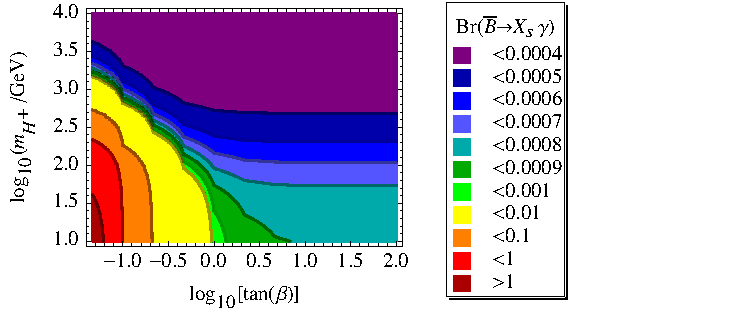
\includegraphics{plots/THDMbsgplot.pdf}}
   \end{picture}
  }
  \caption{An illustration of the tabled values of ${\rm Br}(\bar{B}\to X_s\gamma)$ in dependence of the decadic logarithms of $\tan (\beta)$ and the charged Higgs mass.}
  \label{fig:THDMbsgplot}
\end{figure}

\textbf{$B^-\to \tau \bar{\nu}$ decays}\\

We take the formula from \cite{Hou:1992sy}: the SM branching ratio is proportional to the squared Wilson coefficient, to which we add the THDM contribution

\begin{align}
%CMbtaunu in the code
 C_? &= -4 \frac{G_F}{\sqrt{2}} V_{ub} m_{B^+}^2 \frac{\tan ^2 (\beta)}{m_{H^+}^2}. \nonumber
\end{align}



%%%
%%%\begin{table}
%%%  \centering
%%%  \begin{tabular}{|l|l|c|c|c|c|c|}
%%%    \hline
%%%    \textbf{Theory observable} & \textbf{\HEPfit name} & \textbf{SM} & \textbf{THDM} & \textbf{MSSM} & \textbf{Dim-6} & \textbf{MHC} \\
%%%    \hline
%%%	$\lambda_1$ & \tt{lambda1} & & \checkmark & & &\\
%%%    \hline
%%%	$\lambda_2$ & \tt{lambda2} & & \checkmark & & &\\
%%%    \hline
%%%	$\lambda_3$ & \tt{lambda3} & & \checkmark & & &\\
%%%    \hline
%%%	$\lambda_4$ & \tt{lambda4} & & \checkmark & & &\\
%%%    \hline
%%%	$\lambda_5$ & \tt{lambda5} & & \checkmark & & &\\
%%%    \hline
%%%	\texttt{globalminimum}\:[GeV$^4$] & \tt{globalminimum} & & \checkmark & & &\\
%%%    \hline
%%%	\tt{positivity1} & \tt{positivity1} & & \checkmark & & &\\
%%%    \hline
%%%	\tt{positivity2} & \tt{positivity2} & & \checkmark & & &\\
%%%    \hline
%%%	$\Lambda^{\text{even}}_{21+}$ & \tt{unitarity1} & & \checkmark & & &\\
%%%    \hline
%%%	$\Lambda^{\text{even}}_{21-}$ & \tt{unitarity2} & & \checkmark & & &\\
%%%    \hline
%%%	$\Lambda^{\text{even}}_{01+}$ & \tt{unitarity3} & & \checkmark & & &\\
%%%    \hline
%%%	$\Lambda^{\text{even}}_{01-}$ & \tt{unitarity4} & & \checkmark & & &\\
%%%    \hline
%%%	$\Lambda^{\text{even}}_{00+}$ & \tt{unitarity5} & & \checkmark & & &\\
%%%    \hline
%%%	$\Lambda^{\text{even}}_{00-}$ & \tt{unitarity6} & & \checkmark & & &\\
%%%    \hline
%%%	$\Lambda^{\text{odd}}_{21}$ & \tt{unitarity7} & & \checkmark & & &\\
%%%    \hline
%%%	$\Lambda^{\text{odd}}_{20}$ & \tt{unitarity8} & & \checkmark & & &\\
%%%    \hline
%%%	$\Lambda^{\text{odd}}_{01+}$ & \tt{unitarity9} & & \checkmark & & &\\
%%%    \hline
%%%	$\Lambda^{\text{odd}}_{01-}$ & \tt{unitarity10} & & \checkmark & & &\\
%%%    \hline
%%%	$\Lambda^{\text{odd}}_{00+}$ & \tt{unitarity11} & & \checkmark & & &\\
%%%    \hline
%%%	$\Lambda^{\text{odd}}_{00-}$ & \tt{unitarity12} & & \checkmark & & &\\
%%%    \hline
%%%  \end{tabular}
%%%  \caption{This table summarizes the theory observables of the models
%%%    implemented in the code.}
%%%  \label{tab:summarytheory}
%%%\end{table}
%%%
%%%\begin{table}
%%%  \centering
%%%  \begin{tabular}{|l|l|c|c|c|c|c|}
%%%    \hline
%%%    \textbf{Electroweak precision observable} & \textbf{\HEPfit name} & \textbf{SM} & \textbf{THDM} & \textbf{MSSM} & \textbf{Dim-6} & \textbf{MHC} \\
%%%    \hline
%%%	$\Delta S$ & \tt{DeltaS} & & \checkmark & & &\\
%%%    \hline
%%%	$\Delta T$ & \tt{DeltaT} & & \checkmark & & &\\
%%%    \hline
%%%	$\Delta U$ & \tt{DeltaU} & & \checkmark & & &\\
%%%    \hline
%%%  \end{tabular}
%%%  \caption{This table summarizes the electroweak precision observables of the models
%%%    implemented in the code.}
%%%  \label{tab:summaryewpo}
%%%\end{table}
%%%
%%%\begin{table}
%%%  \centering
%%%  \begin{tabular}{|l|l|c|c|c|c|c|}
%%%    \hline
%%%    \textbf{Higgs observable} & \textbf{\HEPfit name} & \textbf{SM} & \textbf{THDM} & \textbf{MSSM} & \textbf{Dim-6} & \textbf{MHC} \\
%%%    \hline
%%%	$\Gamma_h$ [GeV] & \tt{a} & & \checkmark & & &\\
%%%    \hline
%%%	$r^{(h)}_{\gamma\gamma}$ & \tt{a} & & \checkmark & & &\\
%%%    \hline
%%%	$r^{(h)}_{Z\gamma}$ & \tt{a} & & \checkmark & & &\\
%%%    \hline
%%%	$r^{(h)}_{gg}$ & \tt{a} & & \checkmark & & &\\
%%%    \hline
%%%	$\mu_{\text{\tiny{ggF+tth}}}(h\to bb)$ & \tt{a} & & \checkmark & & &\\
%%%    \hline
%%%	$\mu_{\text{\tiny{VBF+Vh}}}(h\to bb)$ & \tt{a} & & \checkmark & & &\\
%%%    \hline
%%%	$\mu_{\text{\tiny{ggF+tth}}}(h\to WW)$ & \tt{a} & & \checkmark & & &\\
%%%    \hline
%%%	$\mu_{\text{\tiny{VBF+Vh}}}(h\to WW)$ & \tt{a} & & \checkmark & & &\\
%%%    \hline
%%%	$\mu_{\text{\tiny{ggF+tth}}}(h\to \tau \tau)$ & \tt{a} & & \checkmark & & &\\
%%%    \hline
%%%	$\mu_{\text{\tiny{VBF+Vh}}}(h\to \tau \tau)$ & \tt{a} & & \checkmark & & &\\
%%%    \hline
%%%	$\mu_{\text{\tiny{ggF+tth}}}(h\to ZZ)$ & \tt{a} & & \checkmark & & &\\
%%%    \hline
%%%	$\mu_{\text{\tiny{VBF+Vh}}}(h\to ZZ)$ & \tt{a} & & \checkmark & & &\\
%%%    \hline
%%%	$\mu_{\text{\tiny{ggF+tth}}}(h\to \gamma\gamma)$ & \tt{a} & & \checkmark & & &\\
%%%    \hline
%%%	$\mu_{\text{\tiny{VBF+Vh}}}(h\to \gamma\gamma)$ & \tt{a} & & \checkmark & & &\\
%%%    \hline
%%%	$\Gamma^{(H)}_{\text{tot}}$ [GeV] & \tt{a} & & \checkmark & & &\\
%%%    \hline
%%%	$\Gamma^{(H)}_{\gamma\gamma}$ [GeV] & \tt{a} & & \checkmark & & &\\
%%%    \hline
%%%	$\Gamma^{(H)}_{Z\gamma}$ [GeV] & \tt{a} & & \checkmark & & &\\
%%%    \hline
%%%	$\Gamma^{(H)}_{gg}$ [GeV] & \tt{a} & & \checkmark & & &\\
%%%    \hline
%%%	${\rm Br}(H\to hh)$ & \tt{a} & & \checkmark & & &\\
%%%    \hline
%%%	${\rm Br}(H\to AA)$ & \tt{a} & & \checkmark & & &\\
%%%    \hline
%%%	${\rm Br}(H\to H^+H^-)$ & \tt{a} & & \checkmark & & &\\
%%%    \hline
%%%	${\rm Br}(H\to AZ)$ & \tt{a} & & \checkmark & & &\\
%%%    \hline
%%%	${\rm Br}(H\to H^\pm W^\mp)$ & \tt{a} & & \checkmark & & &\\
%%%    \hline
%%%	${\rm Br}(H\to t\bar{t})$ & \tt{a} & & \checkmark & & &\\
%%%    \hline
%%%%%%
%%%%%%\begin{align}
%%%%%%& \sigma ^{(H)}_{\text{\tiny{ggF}}} \cdot {\rm Br}(H\to \tau \tau ) , \quad \sigma ^{(H)}_{\text{\tiny{bbH}}} \cdot {\rm Br}(H\to \tau \tau ), \quad\sigma ^{(H)}_{\text{\tiny{pp}}} \cdot {\rm Br}(H\to \gamma \gamma ) , \quad \sigma ^{(H)}_{\text{\tiny{ggF}}} \cdot {\rm Br}(H\to \gamma \gamma ), \nonumber \\ %C8
%%%%%%%& \sigma ^{(H)}_{\text{\tiny{ggF}}} \cdot {\rm Br}(H\to tt) \nonumber \\ %A8
%%%%%%& \sigma ^{(H)}_{\text{\tiny{bbH}}} \cdot {\rm Br}(H\to bb), \quad \sigma ^{(H)}_{\text{\tiny{ggF}}} \cdot {\rm Br}(H\to WW) , \quad , \quad \sigma ^{(H)}_{\text{\tiny{ggF}}} \cdot {\rm Br}(H\to ZZ), \nonumber \\ %A8
%%%%%%& \sigma ^{(H)}_{\text{\tiny{VBF}}} \cdot {\rm Br}(H\to ZZ), \quad \sigma ^{(H)}_{\text{\tiny{pp}}} \cdot {\rm Br}(H\to VV) /  (\sigma ^{(H)}_{\text{\tiny{pp}}} \cdot {\rm Br}(H\to VV) )_{SM}, \nonumber \\ %C8
%%%%%%& \sigma ^{(H)}_{\text{\tiny{ggF}}} \cdot {\rm Br}(H\to hh) , \quad \sigma ^{(H)}_{\text{\tiny{ggF}}} \cdot {\rm Br}(H\to hh \to (bb)(\tau \tau )), \nonumber \\ %C8
%%%%%%& \sigma ^{(H)}_{\text{\tiny{pp}}} \cdot {\rm Br}(H\to hh \to (bb)(bb)) , \quad \sigma ^{(H)}_{\text{\tiny{pp}}} \cdot {\rm Br}(H\to hh \to (\gamma \gamma )(bb)) \nonumber %C8
%%%%	$\sigma_{\text{ggH}}\!\cdot\! BR(H\!\to\! \tau\tau)$ [pb] & \tt{a} & & \checkmark & & &\\
%%%%    \hline
%%%%	$\sigma_{\text{bbH}}\!\cdot\! BR(H\!\to\! \tau\tau)$ [pb] & \tt{a} & & \checkmark & & &\\
%%%%    \hline
%%%%	$\sigma_{\text{ggH}}\!\cdot\! BR(H\!\to\! \gamma\gamma)$ [pb] & \tt{a} & & \checkmark & & &\\
%%%%    \hline
%%%%	$\mu_{\text{ggH}}(H\!\to\! ZZ)$ [pb] & \tt{a} & & \checkmark & & &\\
%%%%    \hline
%%%%	$\sigma_{\text{ggH}}\!\cdot\! BR(H\!\to\! WW)$ [pb] & \tt{a} & & \checkmark & & &\\
%%%%    \hline
%%%	$R^{(H)}_\text{\tiny Gauss} \left( \sigma ^{(H)}_{\text{\tiny{VBF}}} \cdot {\rm Br}(H\to WW)\right) $ & \tt{Robs\_VBF\_H\_WW\_ATLAS} & & \checkmark & & &\\
%%%    \hline
%%%%	$\sigma_{\text{ggH}}\!\cdot\! BR(H\!\to\! hh)$ [pb] & \tt{a} & & \checkmark & & &\\
%%%%    \hline
%%%%	$\sigma_{\text{ggH}}\!\cdot\! BR(H\!\to\! hh\!\to\! b\bar{b}\tau\tau)$ [pb] & \tt{a} & & \checkmark & & &\\
%%%%    \hline
%%%%	$\sigma_{\text{ppH}}\!\cdot\! BR(H\!\to\! hh\!\to\! b\bar{b}b\bar{b})$ [pb] & \tt{a} & & \checkmark & & &\\
%%%%    \hline
%%%%	$\sigma_{\text{ppH}}\!\cdot\! BR(H\!\to\! hh\!\to\! \gamma\gamma b\bar{b})$ [pb] & \tt{a} & & \checkmark & & &\\
%%%%    \hline
%%%%	$\sigma_{\text{ppH}}\!\cdot\! BR(H\!\to\! t\bar{t})$ [pb] & \tt{a} & & \checkmark & & &\\
%%%%    \hline
%%%%	$\sigma_{\text{bbH}}\!\cdot\! BR(H\!\to\! b\bar{b})$ [pb] & \tt{a} & & \checkmark & & &\\
%%%%    \hline
%%%%	$\Gamma_A$\:[GeV] & $36.29233235$ & $36.91...$ & $36.29233685502$ & $-1.24\cdot 10^{-7}$\\
%%%%	$\Gamma^{(A)}_{\gamma\gamma}$\:[keV] & $115.7310131$ & ? & $115.730932428$ & $6.97\cdot 10^{-7}$\\
%%%%	$\Gamma^{(A)}_{Z\gamma}$\:[keV] & $26.45319592$ & -- & $26.4531773199$ & $7.03\cdot 10^{-7}$\\
%%%%	$\Gamma^{(A)}_{gg}$\:[MeV] & $34.54622361$ & ? & $34.5470976006$ & $-2.53\cdot 10^{-5}$\\
%%%%	${\rm Br}(A\!\to\! HZ)$\:[\%] & $0$ & $0$ & $0$ & $0$\\
%%%%	${\rm Br}(A\!\to\! hZ)$\:[\%] & $0.2266869081$ & $0.2226...$ & $0.226687$ & $1.24\cdot 10^{-7}$\\
%%%%	${\rm Br}(A\!\to\! H^\pm W^\mp)$\:[\%] & $55.35440718$ & $54.58...$ & $55.35440031326$ & $1.24\cdot 10^{-7}$\\
%%%%	${\rm Br}(A\!\to\! t\bar{t})$\:[\%] & $44.245441475$ & ? & $44.24543599800$ & $1.24\cdot 10^{-7}$\\
%%%%	$\sigma_{\text{ggA}}\!\cdot\! BR(A\!\to\! \tau\tau)$\:[ab] & $11.963695367$ & $11.74...$ & $11.40262184364$ & $4.69\cdot 10^{-2}$\\
%%%%	$\sigma_{\text{bbA}}\!\cdot\! BR(A\!\to\! \tau\tau)$\:[zb] & $20.73324124$ & $20.36...$ & $18.01168794027$ & $1.31\cdot 10^{-1}$\\
%%%%	$\sigma_{\text{ggA}}\!\cdot\! BR(A\!\to\! \gamma\gamma)$\:[ab] & $0.4310178090807$ & $1.262...$ & $0.410782470058$ & $4.69\cdot 10^{-2}$\\
%%%%	$\sigma_{\text{ggA}}\!\cdot\! BR(A\!\to\! hZ\!\to\! b\bar{b}\ell\ell)$\:[ab] & $12.3003$ & $12.43...$ & $12.965$ & $-5.40\cdot 10^{-2}$\\
%%%%	$\sigma_{\text{ggA}}\!\cdot\! BR(A\!\to\! hZ\!\to\! b\bar{b}Z)$\:[fb] & $0.182795$ & $0.1847...$ & $0.192599$ & $-5.36\cdot 10^{-2}$\\
%%%%	$\sigma_{\text{ggA}}\!\cdot\! BR(A\!\to\! hZ\!\to\! \tau\tau \ell\ell)$\:[ab] & $2.02201$ & $1.787...$ & $2.13012$ & $-5.35\cdot 10^{-2}$\\
%%%%	$\sigma_{\text{ggA}}\!\cdot\! BR(A\!\to\! hZ\!\to\! \tau\tau Z)$\:[ab] & $20.0219$ & $17.70...$ & $21.0958$ & $-5.36\cdot 10^{-2}$\\
%%%%	$\sigma_{\text{ppA}}\!\cdot\! BR(A\!\to\! t\bar{t})$\:[fb] & $59.9075$ & $60.87...$ & $57.08623$ & $4.71\cdot 10^{-2}$\\
%%%%	$\sigma_{\text{bbA}}\!\cdot\! BR(A\!\to\! b\bar{b})$\:[ab] & $0.16017$ & $0.1573...$ & $0.13916214$ & $1.31\cdot 10^{-1}$\\
%%%  \end{tabular}
%%%  \caption{This table summarizes the Higgs observables of the models
%%%    implemented in the code.}
%%%  \label{tab:summaryhiggs}
%%%\end{table}
%%%
%%%\begin{table}
%%%  \centering
%%%  \begin{tabular}{|l|l|c|c|c|c|c|}
%%%    \hline
%%%    \textbf{Flavour observable} & \textbf{\HEPfit name} & \textbf{SM} & \textbf{THDM} & \textbf{MSSM} & \textbf{Dim-6} & \textbf{MHC} \\
%%%    \hline
%%%	${\rm Br}(\bar{B}\to X_s\gamma)$ & \tt{BR\_bsgamma} & \checkmark & & & &\\
%%%    \hline
%%%	${\rm Br}(\bar{B}\to X_s\gamma)$ & \tt{B\_BtoXsgammaTHDM} & & \checkmark & & &\\
%%%    \hline
%%%	$\Delta m_{B_s}$ & \tt{DmBs} & \checkmark & \checkmark & & &\\
%%%    \hline
%%%	${\rm Br}(B^-\to \tau \bar{\nu})$ & \tt{btaunu} & \checkmark & \checkmark & & &\\
%%%    \hline
%%%  \end{tabular}
%%%  \caption{This table summarizes the flavour observables of the models
%%%    implemented in the code.}
%%%  \label{tab:summaryflavour}
%%%\end{table}

%%%%%
\subsubsection{MSSM}
\label{sec:Flavour:MSSM}
%%%%%

\newcommand{\ljli}{\ell_j \to \ell_i\, \gamma}
\newcommand{\ljtli}{\ell_j \to 3\, \ell_i}
\newcommand{\lilj}{\ell_i \to \ell_j\, \gamma}
\newcommand{\litlj}{\ell_i \to 3\, \ell_j}
%
\newcommand{\hf}{\texttt{HEPfit}}
\newcommand{\lfv}{\texttt{LFV}}
\newcommand{\df}{\Delta F}
%
\newcommand{\C}[1]{\mathcal{C}_{#1\ell}}
\newcommand{\Op}[1]{\mathcal{O}_{#1\ell}}
\newcommand{\Cq}[1]{\mathcal{C}_{#1\ell q}}
\newcommand{\Opq}[1]{\mathcal{O}_{#1\ell q}}
%
\newcommand{\pr}[1]{#1^{\prime}}
%
\newcommand{\gf}{G_F}
%
\newcommand{\meg}{\mu \to e \gamma}

%\subsubsection{MSSM}
%    obsThFactory["mu_e_gamma"] = boost::factory<mu_e_gamma*>();
%    obsThFactory["tau_mu_gamma"] = boost::factory<tau_mu_gamma*>();
%    obsThFactory["tau_e_gamma"] = boost::factory<tau_e_gamma*>();
%    obsThFactory["mu_3e"] = boost::factory<mu_3e*>();
%    obsThFactory["tau_3mu"] = boost::factory<tau_3mu*>();
%    obsThFactory["tau_3e"] = boost::factory<tau_3e*>();
%    obsThFactory["gminus2_mu"] = boost::factory<gminus2_mu*>();

The Higgs sector in MSSM being $Z_2$ symmetric forbids any tree-level flavour changing neutral currents (FCNC). However, this does not preclude the possibility of FCNC decays in general MSSM. The parameters in the soft-SUSY breaking Lagrangian defined in Eq.\eqref{eq:Lsoft_trilinear} and Eq.\eqref{eq:Lsoft_mass} are not necessarily flavour diagonal. For instance, the sfermion masses in Eq.\eqref{eq:Lsoft_mass} are flavor diagonal in gauge mediation~\cite{Dine:1993yw,Dine:1994vc,Dine:1995ag} and gaugino mediation~\cite{Inoue:1991rk,Kaplan:1999ac,Chacko:1999mi} at the leading order. However, in more general cases, e.g. in gravity mediation models, the sfermion mass matrices are not flavour diagonal, that generates various loop-induced FCNC decays. Also, off-diagonal elements of the sfermion mass matrices may arise as results of quantum corrections involving heavy particles, such as right-handed (s)neutrinos~\cite{Borzumati:1986qx, Hisano:1995nq, Hisano:1995cp} and  particles existing in grand unified theories~\cite{Barbieri:1995tw, Moroi:2000mr, Barenboim:2000ev,  Moroi:2000tk}. The present version of \HEPfit calculates various FCNC decays related to the leptonic sector in general MSSM. The SUSY contribution to the quark sector FCNC decays will be added in the future version of \HEPfit.

The \lfv\ module in \hf\ calculates the decay rates for various lepton flavour violating observables in a given new physics model. The expression for various $\df = 1$ and $\df=0$ processes are calculated in terms of the Wilson coefficients of the responsible operators. Therefore, given any new physics model, once the user provides the Wilson coefficients generated in the model, \hf\ will calculate the decay rates for all the lepton flavour violating observables generated by those operators. This enables the user to include any new physics model to \hf\ and analyze the lepton flavour violating processes efficiently. For example, the effective weak Hamiltonian for the $\lilj$ process is given by
\begin{align}
\mathcal{H}_{\rm eff}^{\df=1} &=  
\C{7} \Op{7} + \C{7}^{\prime} \Op{7}^{\prime} , \nonumber
\end{align}
where
\begin{align}
\Op{7} &= e\, m_{l_i} 
\overline{\ell}_j \sigma_{\mu \nu} P_R \ell_i F^{\mu \nu}\ , \notag \\
\Op{7}^{\prime} &= e\, m_{l_i} 
\overline{\ell}_j \sigma_{\mu \nu} P_L \ell_i F^{\mu \nu}\ , \nonumber
\end{align}
$\sigma_{\mu \nu} = \frac{i}{2}[\gamma^{\mu},\gamma^{\nu}]$, $P_{R,L} = \frac{1}{2} (1\pm\gamma_5)$, and $F_{\mu\nu} = (\partial_{\mu} A_{\nu} - \partial_{\nu} A_{\mu})$. $m_{l_i}$ is the mass of the initial state fermion. The decay rate for the process is
\begin{align}
\Gamma (\lilj) &= \frac{e^2}{4\pi} m_{l_i}^5 
\bigg(|\C{7}|^2 + |\C{7}^\prime|^2\bigg) \ . \nonumber
\end{align}

\begin{itemize}
	\item Anomalous magnetic moment of muon ($(g-2)_{\mu}$): At one-loop the contribution from the supersymmetric particles to $(g-2)_{\mu}$ is through neutralino--charged slepton loop and chargino--sneutrino loop \cite{Chattopadhyay:1995ae,Moroi:1995yh,Hisano:1995cp}. In \hf\ the two-loop contribution to $(g-2)_{\mu}$ is also computed. The following two-loop corrections  are included in the present version of \hf\ :
		(1) $\tan\beta$-enhanced corrections to the muon Yukawa coupling \cite{Marchetti:2008hw},
		(2) QED corrections to the SUSY contributions to the muon $g-2$ \cite{vonWeitershausen:2010zr} (for the leading term, see also \cite{Degrassi:1998es}),
		(3) leading logarithmic corrections from fermion/sfermion loops \cite{Fargnoli:2013zia}, which are enhanced for heavy sfermions,
		(4) corrections from photonic Barr-Zee diagrams involving the neutral Higgs bosons with charginos or sfermions \cite{Stockinger:2006zn}, which are enhanced by $\tan\beta$ or potentially large Yukawa couplings.
		The first three corrections can be regarded as corrections to one-loop SUSY contributions.
	\item $\lilj$ decay: At one-loop in MSSM the $\lilj$ decay is mediated through the neutralino-charged slepton and the chargino-sneutrino loop. In the present version of \hf\ we include the contribution to $\lilj$ in the general MSSM scenario \cite{Hisano:1995cp}, keeping the final final state fermion masses non-zero \cite{Arganda:2005ji}.
	\item $\litlj$ decay: In the general MSSM, the $\litlj$ receives contribution from $\gamma$, $Z$ and $H$-penguin type and box-type diagrams. The present version of \hf\ includes all of these 4-types of contribution for finite final state fermion masses \cite{Hisano:1995cp,Arganda:2005ji}. 
	\item Coherent $\mu \to e$ conversion in nuclei: The coherent $\mu \to e$ conversion in a nucleus corresponds to the process $X_{\mu}(Z,A) \to e^{-} + X^{+}(Z,A)$, where $X_{\mu}(Z,A)$ is an atom of nucleus $X$ with proton number $Z$ and atomic number $A$ with one orbital electron replaced by a muon and $X^{+}(Z,A)$ is the corresponding ion without the muon. The coherent $\mu \to e$ conversion receives contribution from $\gamma$, $Z$-penguin-type and box-type diagrams \cite{Hisano:1995cp}. Present version of \hf\ includes both of these contribution in the general MSSM scenario.  
\end{itemize}

%%%%%%%%%%%%%%%%%%%%%%%%%%%%%%%%%%%%%
\section{Code Description}
\label{sec:Code}
%%%%%%%%%%%%%%%%%%%%%%%%%%%%%%%%%%%%%

L+M+E, Ayan


\newpage

%%%%%%%%%%%%%%%%%%%%%%%%%%%%%%%%%%%%%
\section{Installation}
\label{sec:Installation}
%%%%%%%%%%%%%%%%%%%%%%%%%%%%%%%%%%%%%

We give a brief description of the installation procedure here. The installation depends on the availability of \texttt{cmake} on the system. A description of cmake and the details of installing it can be found in \href{https://cmake.org/}{the cmake website}. Most package managers for linux distributions should have an package available for installation. For Mac users, it can be either installed from source or from a Unix port like \href{https://www.macports.org/}{Darwin ports} or \href{http://www.finkproject.org/}{Fink}. Below we outline further details. 

\subsection{Dependencies}

\begin{itemize}
\item {\bf GSL:}  The GNU Scientific Library (GSL) is a library for numerical computation. It can be found on the \href{http://www.gnu.org/software/gsl/}{GSL website}. Most linux package managers will have a stable version as will any ports for Mac. {\bf NOTE:} We do not support GSL v2.0 or greater. 

\item {\bf ROOT v5 or later:}  ROOT is an object oriented data analysis framework. You can obtain it from the \href{http://root.cern.ch/}{ROOT website}.

\item {\bf BOOST:}  BOOST is a C++ library. You can obtain it from the \href{http://www.boost.org}{BOOST website} or from linux package managers or Mac ports. While we do not need the BOOST libraries, we do need the headers, so one should make sure the headers are installed and not the libraries only. 

\item {\bf BAT v0.9.4 (not required for the Library mode):} Optionally, BAT (Bayesian Analysis Toolkit) can be obtained from 
    the \href{https://www.mppmu.mpg.de/bat/}{BAT website} for a Monte Carlo run. With the compilation 
    option \texttt{-DBAT\_INSTALL=ON} explained below, the \HEPfit installation package 
    will download and install BAT. {\bf NOTE:} that at present \HEPfit is not
    compatible with BAT compiled with the \texttt{--enable-parallelization} option. the parallelized version of BAT compatible with \HEPfit\ {\em must} be installed with the option \texttt{-DMPIBAT=ON}

\item {\bf MPI:}    Optionally, HEPfit can be compiled with MPI for usage in parallel 
    clusters and processors supporting multi-threading. In this case,
    the \HEPfit installer will patch and compile BAT with MPI support as described above. For this one needs a version of \href{https://www.open-mpi.org/}{openMPI} which is also available through package managers in Linux and ports on Mac.
\end{itemize}

\subsection{Installation Procedure}

In a nutshell, if all dependencies are satisfied for a fully MPI compatible MCMC capable \HEPfit installation from the tarball downloaded from \href{http://hepfit.roma1.infn.it/}{the \HEPfit website}:

\begin{lstlisting}
$ tar xvzf HEPfit-x.x.tar.gz
$ mkdir HEPfit-x.x/build 
$ cd HEPfit-x.x/build 
$ cmake .. -DLOCAL_INSTALL_ALL=ON -DMPIBAT=ON
$ make
$ make install
\end{lstlisting}
To run your first example:
\begin{lstlisting} 
$ cd examples/MonteCarloMode/
$ make  
$ mpiexec -n 5 ./analysis ../config/StandardModel.conf MonteCarlo.conf
\end{lstlisting} 
This is all you will need for running a MCMC on 5 cores with the model, parameters and observables specified in \texttt{examples/config/StandardModel.conf} with \HEPfit. For variations please read what follows. \\\\
%
Unpack the tarball containing the \HEPfit source which you can obtain from the \href{http://hepfit.roma1.infn.it/}{\HEPfit website}. A directory called 
\texttt{HEPfit-x.x} will be created containing the source code. To generate 
Makefiles, enter the source directory and run CMake:

\begin{lstlisting}
$ cd HEPfit-x.x  
$ cmake . <options>  
\end{lstlisting}

{\bf (RECOMMENDED:)} Alternatively, a directory separate from the source directory can be made for
building \HEPfit (recommended as it allows for easy deletion of the build):
\begin{lstlisting}
$ mkdir HEPfit-x.x/build  
$ cd HEPfit-x.x/build  
$ cmake .. <options>  
\end{lstlisting}

where the available options are:

\begin{itemize}
\item \texttt{-DLOCAL\_INSTALL\_ALL=ON}: to install BAT and \HEPfit in the current directory (default: OFF). 
    This is equivalent in setting the options \texttt{-DCMAKE\_INSTALL\_PREFIX=./HEPfit}, 
    \texttt{-BAT\_INSTALL\_DIR=./BAT} and \texttt{-DBAT\_INSTALL=ON}, where these variables cannot 
    be modified individually when \texttt{-DLOCAL\_INSTALL\_ALL=ON} is set. 

\item \texttt{-DCMAKE\_INSTALL\_PREFIX=<HEPfit installation directory>}: the directory in which \HEPfit will be installed (default: \texttt{/usr/local})  
  
\item \texttt{-DNOMCMC=ON}: to enable the mode without MCMC (default: OFF)

\item \texttt{-DDEBUG\_MODE=ON}: to enable the debug mode (default: OFF)

\item \texttt{-DBAT\_INSTALL\_DIR=<BAT installation directory>}: (default: \texttt{/usr/local}). This option is overruled by \texttt{-DLOCAL\_INSTALL\_ALL=ON}

\item \texttt{-DBAT\_INSTALL=ON} to download and install BAT (default: OFF)

\item \texttt{-DMPIBAT=ON}: to enable support for MPI
    (requires an implementation of MPI, default: OFF)

\item \texttt{-DMPI\_CXX\_COMPILER=<path to mpi>/mpicxx}: You can specify the MPI compiler with this option

\item \texttt{-DBOOST\_INCLUDE\_DIR=<boost custom include path>/boost/}: if BOOST is not installed in the search path then you can specify where it is with this option. The path must end with the \texttt{boost/} directory which contains the headers.

\item \texttt{-DGSL\_CONFIG\_DIR=<path to gsl-config>}: \HEPfit used \texttt{gsl-config} to get the GSL parameters. If this is not in the search path, you can specify it with this option. 

\item \texttt{-DROOT\_CONFIG\_DIR=<path to root-config>}: HEPfit used \texttt{root-config} to get the ROOT parameters. If this is not in the search path, you can specify it with this option. 
\end{itemize}
Setting the option \texttt{-DBAT\_INSTALL=ON}, the \HEPfit installer will download, 
compile and install the BAT libraries.\\\\
%
{\bf NOTE:}
Please make sure that the BAT libraries are not already present in the
BAT installation directory. If it is present, the installer does not
build BAT, and uses the pre-installed one. This is particularly problematic
if switching to or from the MPI version of BAT (\texttt{-DMPIBAT=ON}).\\\\
%
{\bf No MCMC mode:}
The generated Makefiles are used for building a \HEPfit library. If
you do not perform a Bayesian statistical analysis with the Markov
Chain Monte Carlo (MCMC), you can use the option \texttt{-DNOMCMC=ON}. For
this case, BAT is not required. \\\\
%
{\bf MPI Support:}
If you want to perform an MCMC run with MPI support, you can specify
the option \texttt{-DMPIBAT=ON}. This option must be accompanied with
\texttt{-DBAT\_INSTALL=ON} in order to enable the \HEPfit installer to
download, patch and compile BAT with MPI support:
\begin{lstlisting} 
$ cmake . -DBAT_INSTALL=ON -DMPIBAT=ON <other options>  
\end{lstlisting}
Please make sure non-MPI BAT libraries are not already installed in the 
BAT installation directory.\\\\
%
{\bf ROOT:}
CMake checks for ROOT availability in the system and fails if ROOT is
not installed. You can specify the path to root-config using the
option \texttt{-DROOT\_CONFIG\_DIR=<path to root-config>}. \\\\
%
{\bf BOOST:}
CMake also checks for BOOST availability in the system and fails if
BOOST is not installed. You can specify the path to the BOOST include
files with \texttt{-DBOOST\_INCLUDE\_DIR=<boost custom include path>/boost/}. \\\\
%
The {\bf recommended installation} flags for a locally installed \HEPfit with full MPI and MCMC support is:
\begin{lstlisting} 
$ cmake . -DLOCAL_INSTALL_ALL=ON -DMPIBAT=ON
\end{lstlisting}
This will enable easy portability of all codes and easy upgrading to future version as nothing will be installed system wide.  Also, this is useful if you do not have root access and cannot install softwares in system folders. After successful CMake run, execute the build commands:

\begin{lstlisting} 
$ make  
$ make install  
\end{lstlisting} 
to compile and install \HEPfit, where the command \texttt{make VERBOSE=1}
enables verbose output and \texttt{make -j} allows for parallel compilation.
Note that depending on the setting of installation prefix you might
need root privileges to be able to install \HEPfit with \texttt{sudo make
install} instead of just \texttt{make install}.\\

\subsection{Post Install:}

\begin{itemize}
\item{\bf Executable:} \texttt{<CMAKE\_INSTALL\_PREFIX>/bin/hepfit-config}
\item{\bf Library:} \texttt{<CMAKE\_INSTALL\_PREFIX>/lib/libHEPfit.a}
\item{\bf Combined Header:} \texttt{<CMAKE\_INSTALL\_PREFIX>/include/HEPfit/HEPfit.h}
\end{itemize}

{\bf Using hepfit-config:}
A hepfit-config script can be found in the \texttt{<CMAKE\_INSTALL\_PREFIX>/bin/}
directory, which can be invoked with the following options:
\begin{itemize}
\item \texttt{--cflags} to obtain the include path needed for compilation against the \HEPfit library

\item \texttt{--libs} to obtain the flags needed for linking against the \HEPfit library
\end{itemize}

{\bf Examples:}

The example programs can be found in the \HEPfit build directory:  
\begin{itemize}
\item \texttt{examples/LibMode\_config/}  
\item \texttt{examples/LibMode\_header/} 
\item \texttt{examples/MonteCarloMode/}
\item \texttt{examples/EventGeneration/}
\item \texttt{examples/myModel/}
\end{itemize}
The first two demonstrate the usage of the \HEPfit library, while 
the third one can be used for testing a Monte Carlo run with the \HEPfit 
executable. The fourth example can be used to generate values of observables with a sample of parameters drawn from the parameter space. The fifth one is an example implementation of a custom 
model and custom observables. To make an executable to run these examples:
\begin{lstlisting} 
$ cd examples/MonteCarloMode/
$ make  
\end{lstlisting} 
This will produce an executable called \texttt{analysis} in the current directory that can be used to run \HEPfit. The details are elaborated on in the next section.



%%%%%%%%%%%%%%%%%%%%%%%%%%%%%%%%%%%%%
\section{Usage and Examples}
\label{sec:Usage}
%%%%%%%%%%%%%%%%%%%%%%%%%%%%%%%%%%%%%
The HEPfit installer generates the 
library \texttt{libSufyFit.a} along with header files including a combined
header file, \texttt{HEPfit.h}. To perform a Bayesian statistical analysis with the
Markov Chain Monte Carlo one can use the given example implementation.
Alternatively, one can use the library to obtain predictions
of observables for a given point in the parameter space of the model, 
allowing our computational tool to be called from the user's own program. We explain both the methods in the following discourse. 

%%%%%%%%%%%%%%%%%%%%%%%%%%%%%%%%%%%%%
\subsection{Monte Carlo Mode}
\label{sec:MC}
%%%%%%%%%%%%%%%%%%%%%%%%%%%%%%%%%%%%%

The Monte Carlo analysis is performed with the BAT library. First,
a text configuration file containing a list of model parameters,
model flags and observables to be analyzed has to be prepared. Another configuration
file for the Monte Carlo run has to be prepared, too.\\\\
%
{\bf \large Step 1: Model configuration file}\\


The configuration files are the primary way to control the behavior of the code and to detail its input and output. While a lot of checks have be implemented in \HEPfit to make sure the configuration files are of the right format, it is not possible to make it error-proof. Hence, much care should be taken to prepare these files.A configuration file for model parameters, model flags and
observables are written as follows:\\

\lstinputlisting[language=C++]{codes/ModelConf.conf}
where the lines beginning with the `\#' are commented out. Each line has to be written as follows: 

\begin{enumerate}
\item The first line must be {\bf the name of the model} to be analyzed,
   where the available models are listed in the page @ref PageModels.
  
\item  {\bf A model parameter} is given in the format:
\begin{lstlisting}
ModelParameter <name> <central value> <Gaussian error> <flat error>`
\end{lstlisting}
where all the parameters in a given model (see @ref PageModels) have
  to be listed in the configuration file.

\item {\bf A set of correlated model parameter} is specified with 
\begin{lstlisting}
CorrelatedGaussianParameters name Npar
\end{lstlisting}
   which initializes a set of Npar correlated parameters. It must be
   followed by exactly Npar Parameter lines and then by Npar lines of
   Npar numbers for the correlation matrix. See the above example.

\item  Optionally, one can set {\bf a model flag} in the format:

\begin{lstlisting}
ModelFlag <name> <value>
\end{lstlisting}

  where the available flags for a given model can be found in the page
  @ref PageModels.

\item  {\bf An observable} to be computed is specified in one of the following formats:
\begin{lstlisting}
Observable <name> <obs label> <histolabel> <min> <max> (no)MCMC (no)weight <central value> <Gaussian error> <flat error>
#
Observable <name> <obs label> <histolabel> <min> <max> (no)MCMC file <filename> <histoname>
#
Observable <name> <obs label> <histolabel> <min> <max> noMCMC noweight
\end{lstlisting}
\begin{itemize}
  \item {\bf \texttt{<name>}} is user given name for different observables which must be unique for each observable
  \item {\bf \texttt{<obs label>}} is the theory label of the observable (see @ref PageModels).
  \item {\bf \texttt{<histolabel>}} is used for the label of the output ROOT histogram,
  while {\bf \texttt{<min>}} and {\bf \texttt{<max>}} represent the range of the histogram.
  \item  {\bf \texttt{(no)MCMC}} is the flag specifying whether the observable should be included in the Monte Carlo prerun or not 
  \item {\bf \texttt{(no)weight}} specifies if the observable weight will be computed or not. If weigh is specified with noMCMC
    then the weight of the observable will be stored in the MCout*.root file
  \item Experimental data is specified as {\bf \texttt{<central value>  <Gaussian error>  <flat error>}}. If weight is specified
    both the errors cannot be 0.
  \item A histogram in a ROOT file is specifed by the name of the root file ({\bf \texttt{filename}}) and then the
    name of the histogram ({\bf \texttt{histoname}}).
\end{itemize}

\item  {\bf Correlations among the data of observables} can be taken into
   account with the line "CorrelatedGaussianObservables name Nobs",
   which initializes a set of Nobs correlated observables. It must be
   followed by exactly Nobs Observable lines and then by Nobs lines of
   Nobs numbers for the correlation matrix. See the above example.
   One can use the keyword noMCMC and noweight, instead of MCMC and weight.

\item  {\bf A correlation between two observables} can be obtained with any of the four following specifications: 

\begin{lstlisting}
Observable2D <name> <obs1 label> <histolabel1> <min1> <max1> noMCMC noweight <obs2 label> <histolabel2> <min2> <max2>
#
Observable2D <name> <obs1 label> <histolabel1> <min1> <max1> MCMC file <filename> <histoname> <obs2 label> <histolabel2> <min2> <max2>
#
Observable2D <name> (no)MCMC (no)weight
(Binned)Observable <obs label 1> <histolabel 1> <min> <max> <central value> <Gaussian error> <flat error> (<bin_min> <bin_max>)
(Binned)Observable <obs label 2> <histolabel 2> <min> <max> <central value> <Gaussian error> <flat error> (<bin_min> <bin_max>)
#
Observable2D <name> MCMC file filename histoname
(Binned)Observable <obs label 1> <histolabel 1> <min> <max> (<bin_min> <bin_max>)
(Binned)Observable <obs label 2> <histolabel 2> <min> <max> (<bin_min> <bin_max>)
\end{lstlisting}

\item  {\bf Include configuration files} with the IncludeFile directive. This is useful if one
   wants to separate the input configurations for better organization and flexibility.

\end{enumerate}
%
{\bf \large Step 2: Monte Carlo configuration file:}\\

The parameters and options of the Monte Carlo run are specified in
a configuration file, separate from the one for model parameters,
etc. Each line in the file has a pair of a label
and its value, separated by space(s) or tab(s). The available
parameters and options are: \\\\
{\bf NChains} : The number of chains in the Monte Carlo run. A minimum of 5 is suggested (default). 
If the theory space is complicated and/or the number of parameters are large then more
is necessary. The amount of statistics collected in the main run is proportional to the
numbe rof chains.\\\\
{\bf PrerunMaxIter} : The maximum number of iterations that the prerun will go through (default: 1000000). 
The prerun ends automatically when the chains converge (R$<$1.1) and all efficiencies 
are adjusted. While it is not necessary for the prerun to converge for a run to be 
successful, one should exercise caution in this case.\\\\
{\bf Iterations} : The number of iterations in the main run. This run is for the purpose of
collecting statistics and is at the users discretion. (default: 100000)\\\\
{\bf Seed} : The seed can be fixed for deterministic runs.\\\\
{\bf PrintAllMarginalized} : All marginalized distributions will be printed in a pdf file
(MonteCarlo\_plots\_*.pdf).\\\\
{\bf PrintCorrelationMatrix} : The parametric corellation will be printer in ParamCorrelations*.pdf
and ParamCorrelations*.tex.\\\\
{\bf PrintKnowledgeUpdatePlots} : A comparison between prior and posterior knowledge will be 
printed in a plot stored in ParamUpdate*.pdf.\\\\
{\bf PrintParameterPlot} : As summary of the paramters will be printed in ParamSummary*.pdf.\\\\
{\bf OrderParameters} : This determines whether the parameters will be randomized one
at a time or as a whole set in the entire run. While for quick estimates it is not necessary
to order the prameters (false), it is suggested to do so for more accurate estimates.\\\\
{\bf FindModeWithMinuit} : To find global mode with MINUIT starting
from the best fit parameters in the MCMC run.\\\\
{\bf MinimumEfficiency}  : This allows the setting of the minimum eifficiency of 
all the prameters. The default is 0.15.\\\\
{\bf WriteChain}        : The chains will be written in the root file MCout*.root. 
This can be used for analyzing the performance of the chains.\\\\
{\bf CalculateNormalization} : The normalization of the theory space will be calculated
at the end of the Monte Carlo run. This is useful for model comparison.\\\\
{\bf WritePreRunData} : The prerun data is written to a file for rerun.      \\\\
{\bf ReadPreRunData}  : The prerun data will be read from a previously stored prerun file. \\\\
For example, a Monte Carlo configuration file is written as: 

\lstinputlisting[language=C++]{codes/MCMC.conf}

where a '\#' can be placed at the beginning of each line to comment it out.\\\\
%
{\bf \large Step 3: Run}\\\\
%
{\bf 1. Library mode with MCMC:  }An example can be found in examples/MonteCarloMode

\begin{lstlisting}
  $ cd examples/MonteCarloMode
  $ make
\end{lstlisting}

After making the configuration files, run with the command:
\begin{lstlisting}
  $ ./analysis <model conf> <Monte Carlo conf>
\end{lstlisting}
%
{\bf Alternative: Run with MPI}\\ \HEPfit allows for parallel processing of the MCMC run and the observable computations.
To allow for this \HEPfit and BAT has to be compiled with MPI support as explained in the
@ref PageInstallation page. The command

\begin{lstlisting}
  $ mpiexec -n N ./analysis <model conf> <Monte Carlo conf>
\end{lstlisting}

will launch analysis on `N` thread/cores/processors depending on the smallest
processing unit of the hardware used. Our MPI implementation allows for runs on multi-threaded single processors as
well as clusters with MPI support.\\\\
%
{\bf NOTE:} Our MPI implementation of \HEPfit cannot be used with
BAT compiled with the \texttt{--enable-parallelization} option. It is
mandatory to use the MPI patched version of BAT as explained in the @ref PageInstallation page.\\


{\bf Output Files:}
\begin{itemize}
\item log.txt: This is the log file.
\item MCout.root: This is the root file containing all the information of the run and
  the histogram objects.
\item MonteCarlo\_results.txt: This file contains the fits to the parameters.
\item MonteCarlo\_plots.pdf: This File contains the histograms for the parameters.
\item Observables: This directory will contain the histograms of all the observables
  specified in the config file.
\item Observables/HistoLog.txt: This file contains the information on over-run and under-run
  of the histogram filling.
\item Observables/Statistics.txt: This file contains the compilation of the statistics
  extracted from the histograms.
\end{itemize}
Other files might be generated depending on the options specified in the Monte Carlo 
configuration file.\\\\
%
%%%%%%%%%%%%%%%%%%%%%%%%%%%%%%%%%%%%%
\subsection{Event Generation Mode}
\label{sec:MC}
%%%%%%%%%%%%%%%%%%%%%%%%%%%%%%%%%%%%%
Using the model configuration file used in the Monte Carlo mode, one
can obtain predictions of observables. An example can be found in \texttt{examples/EventGeneration} folder

\begin{lstlisting}
  $ cd examples/EventGeneration
  $ make
\end{lstlisting}

After making the configuration files, run with the command:
\begin{lstlisting}
  $ ./analysis <model conf> <number of iterations> [output folder]
\end{lstlisting}

The \texttt{<number of iterations>} defines the number of random points in the parameter space that will be evaluated. Setting this to 0 gives the value of the observables at the central value of all the parameters. If the \texttt{[output folder]} is not specified everything is printed on the screen and no data is saved. Alternately, one can specify the output folder and the run will be saved if \texttt{<number of iterations>} $>$ 0. The output folder can be found in \texttt{./GeneratedEvents}. The structure of the output folder is:\\\\
%
{\bf Output folder structure:}
\begin{itemize}
\item \texttt{CGO}: Contains any correlated Gaussian observables that might have been listed in the model configuration files.
\item \texttt{Observables}: Contains any observables that might have been listed in the model configuration files.
\item \texttt{Parameters}: Contains all the parameters that were varied in the model configuration files.
\item \texttt{Summary.txt}: Contains a list of the model used, the parameters varied, the observables computed and the number of events generated. This can be used, for example, to access all the files from a third party program.
\end{itemize}
The parameters and the observables are stored in the respective directories in files that are names after the same. For example, the parameter \texttt{lambda} will be saved in the file \texttt{lambda.txt} in the \texttt{Parameters} folder.


%
%%%%%%%%%%%%%%%%%%%%%%%%%%%%%%%%%%%%%
\subsection{Library mode without MCMC}
\label{sec:MC}
%%%%%%%%%%%%%%%%%%%%%%%%%%%%%%%%%%%%%
The library mode allows for access to all the observables implemented in HEPfit
without a Monte Carlo run. The users can use one of our defined @ref PageModels and vary ModelParameters
according to their own algorithm and get the corresponding predictions for the observables. This is made possible through:
\begin{itemize}
\item a combined library: \texttt{libHEPfit.a} (installed in \texttt{HEPFIT\_INSTALL\_DIR/lib})
\item a combined header file: \texttt{HEPfit.h} (installed in \texttt{HEPFIT\_INSTALL\_DIR/include/HEPfit})
\end{itemize}
The HEPfit library allows for two different implementations of the access algorithm.\\\\
%
{\bf Non-Minimal Mode:}

In the non-minimal mode the user can use the SomeModel.conf file to pass the default value of
the model parameters. The following elements must be present in the user code to define
the parameters and access the observable. (For details of model parameters, observables etc. please lookup @ref PageModels.)

\lstinputlisting[language=C++]{codes/nonMinimal.cpp}
%
{\bf Minimal Mode:}

In the minimal mode the user can use the default values in InputParameters header file to define the
default values of the model parameters therefore not requiring any additional input files to be
parsed. (For details of model name, flags, parameters, observables etc. please lookup @ref PageModels.)

\lstinputlisting[language=C++]{codes/Minimal.cpp}
%
{\bf Use of hepfit-config:} If \texttt{make install} has been done, a hepfit-config script can be found in the
\texttt{HEPFIT\_INSTALL\_DIR/bin} directory, which can be invoked with the 
following options:

\begin{lstlisting}
Library and Library Path: hepfit-config --libs

Include Path: hepfit-config --cflags
\end{lstlisting}

The last command lists all the mandatory parameters in all the models sorted alphabetically and their
default values as set in the class InputParameters.
%%%%%%%%%%%%%%%%%%%%%%%%%%%%%%%%%%%%%
\section{Comparison with Other Codes}
\label{sec:Comparison}
%%%%%%%%%%%%%%%%%%%%%%%%%%%%%%%%%%%%%

%%%%%%%%%%%%%%%%%%%%%%%%
\subsection{Comparison with ZFITTER}
\label{sec:ZFitter}
%%%%%%%%%%%%%%%%%%%%%%%%

\satoshisnotes{%2
%otto:
The pseudo $Z$-pole observables introduced in section \ref{sec:EWPO} are in good agreement with the ones calculated with the ZFITTER setup \cite{Bardin:1992jc,Bardin:1999yd,Arbuzov:2005ma,Akhundov:2013ons} with relative errors well below the relative experimental uncertainty.
%satoshi:
It is noted that we keep only one-loop contributions in the imaginary
parts. A relatively larger difference in Re$(\rho_Z^b)$ is due to the
fact that the one-loop remainder contribution in Re$(\rho_Z^b)$ is
defined with the coupling $\alpha(0)$ in ZFITTER, while 
$G_\mu$ has been adopted in \HEPfit.
The small difference in Re$(\kappa_Z^b)$ originates from the
fact that ZFITTER does not use the two-loop approximate formula for 
$\sin^2\theta_{\rm eff}^b$. Moreover, 
the differences in Im$(\kappa_Z^f)$ are attributed
to the $O(\alpha\alpha_s)$ term in ZFITTER codes: 
\begin{align}
{\rm Im}(\kappa_Z^f) &= 
{\rm Im}(\delta\kappa_{\rm rem}^{f,\alpha})
- \frac{\alpha(0)\alpha_s(M_Z^2)}{24\pi}
  \frac{\left( c_W^2- s_W^2 \right)}{s_W^4}\,. 
\end{align}

}%satoshisnotes %2

%%%%%%%%%%%%%%%%%%%%%%%%
\subsection{Comparison with UTfit}
\label{sec:UTfit}
%%%%%%%%%%%%%%%%%%%%%%%%

L+M+E

%%%%%%%%%%%%%%%%%%%%%%%%
\subsection{Comparison with JDBM}
\label{sec:JDBM}
%%%%%%%%%%%%%%%%%%%%%%%%

Jorge

%%%%%%%%%%%%%%%%%%%%%%%%
\subsection{Comparison with SuSeFLAV}
\label{sec:Debtosh}
%%%%%%%%%%%%%%%%%%%%%%%%

Debtosh

%%%%%%%%%%%%%%%%%%%%%%%%
\subsection{Comparison with the THDM implementation in CKMfitter}
\label{sec:CKMfitter}
%%%%%%%%%%%%%%%%%%%%%%%%

All THDM observables were compared to the CKMfitter implementation used in \cite{Eberhardt:2013uba,Eberhardt:2013wia,Baglio:2014nea,Chowdhury:2015yja}. For most of them, the relative difference was less than $10^{-9}$, except for the heavy Higgs search observables, where HEPfit uses updated reference tables for the cross sections, and no interpolation was used on the CKMfitter side, such that the relative error amounts to maximally a few percent, which we assume to be sufficient given the experimental precision.




\section*{Acknowledgments}
M.C. is associated to the Dipartimento di Fisica, Universit\`a di Roma
Tre. E.F. and L.S. are associated to the Dipartimento di Fisica,
Universit\`a di Roma ``La Sapienza''. We acknowledge partial support
from ERC Ideas Starting Grant n.~279972 ``NPFlavour'' and ERC Ideas
Advanced Grant n.~267985 ``DaMeSyFla''.















%% The Appendices part is started with the command \appendix;
%% appendix sections are then done as normal sections
%% \appendix

%% \section{}
%% \label{}

\bibliographystyle{elsarticle-num}
\bibliography{HEPfit-1.0}

\end{document}
